\documentclass[12pt, a4 paper]{article}

\usepackage{My_packages}
%\usepackage[utf8]{inputenc}
%\usepackage{xcolor}

\definecolor{dg}{rgb}{0.0, 0.6, 0.1}
\newcommand{\Andrew}[1]{\textcolor{dg}{#1}}
\newcommand{\Arjen}[1]{{\color{brown}#1}}
\newcommand{\Vasu}[1]{{\color{purple}#1}}


\date{ }

\begin{document}
\iffalse
\begin{titlepage}
    Paper Rough draft
\end{titlepage}
\fi

\tableofcontents
\newpage

\section{Introduction}
\label{Introducion}

% What do we know about magnetic fields?   
The origin and structure of the Galactic magnetic field remains a long standing unresolved problem in astrophysics. What is apparent, however, is the vital role it plays, especially in terms of cosmic ray propagation within the Galaxy. The incompleteness of the observational data, required to probe the Galactic magnetic field structure on many different scales, limits significantly our ability to describe cosmic ray propagation through the Galaxy. This is especially true when it comes to the modelling of cosmic ray propagation out in the Galactic halo where our knowledge of the magnetic field is particularly weak.

%  tools used to detect magnetic fields namely RM and synchrotron. And typical values for these fields
A variety of methods allow observational probes of Galactic magnetic fields, such as starlight polarisation and infrared emission from dust grains, or Zeeman splitting of spectral radio lines in the dust clouds \textcolor{blue}{\cite{Beck_2007}}. Galactic magnetic fields are also probed by Pulsar dispersion with Faraday rotation, which is sensitive to the magnetic-field component parallel to the line of sight $B_{\parallel}$, and synchrotron radiation which probes the component perpendicular to the line of sight $B_{\perp}$. A major drawback in using the Pulsar dispersion measure along with the Faraday rotation measure method for probing Galactic magnetic fields is that it relies heavily on the lines of sight along which Pulsars are found, which places a strong focus on the regions close to the Galactic plane. Therefore, this method is of most use for probing the magnetic field in the Galactic disc region, and is not so useful for probing the magnetic field out in the Galactic halo. Synchrotron radiation on the other hand is produced via the gyration of non-thermal electrons along magnetic field lines. This method can thus be used to probe magnetic fields also in the Galactic halo.

\Vasu{We should first talk about the Fermi observations and then SPASS and the model.}
% Observations from Fermi 
The observations from FERMI-LAT \cite{Su_2010} in the gamma ray regime unveiled giant bipolar gamma ray bubbles extending up to $\approx$~3~kpc radially and $\approx$~8~kpc in the z-direction, having a total energy of $\approx 10^{(54-55)}$~ergs. Recently, observations from eROSITA \cite{eROSITA} in X-ray regime further suggest existence of even larger bubbles going up to  $\approx$~7~kpc radially and $\approx$~14~kpc in the azimuthal direction, having a total energy of $\approx 10^{(56)}$~ergs. These observations strongly motivate the requirement of a magnetic field model focusing on the halo. Henceforth, for the sake of simplicity we will address the two bubbles together as the Galactic halo bubbles.

% Observations from S-PASS and Planck
With the help of the aforementioned techniques, we can estimate the strength and direction of the magnetic field in different parts of the Galaxy. 
For the Galactic halo the S-PASS \cite{Carretti_2013} observations  made at 2.3 GHz seem to suggest that the field strength in the halo bubbles can be anywhere between $6-10~\mu $G depending on the proton-electron ratio. S-PASS \cite{Carretti_2013} observation however are subject to depolarisation of polarised synchrotron radiation via Faraday rotation due to its low observation frequencies and this data set is also not sensitive to a portion of the Fermi bubbles because of its positioning in the southern hemisphere. For this reason data from Planck and WMAP are more helpful when probing magnetic fields in the Galactic halo due to their all sky coverage and observation bandwidths which are not sensitive to Faraday rotation effects.

% Other magnetic field models and energies in the halo.

Several efforts have  been made in modelling magnetic fields in the Galaxy namely by \cite{Jaffe_2010},\cite{Jaffe_2011}, \cite{Sun_2008},and \cite{JF12}. It should be noted that our understanding for Galactic disc is much better than the halo due to larger amount of observational data present at varying frequencies. However, widely used models like JF12 \cite{JF12} have made considerable contributions also towards modelling of Galactic halo. One drawback with JF12 \cite{JF12} is that they mask out the Fermi bubble regions in their models but, S-PASS\cite{Carretti_2013} observations tell us that magnetic field strength in this region is not negligible. Therefore, it is important to consider modelling the Galactic halo including the Fermi bubbles.


% Short note on non-thermal electron distribution.
\Vasu{This paragraph needs more work}
Apart from the Galactic magnetic field, our understanding of the non-thermal electron distribution in the Galaxy is also poor. We have some information on the distribution of cosmic ray electrons from the observations made by \Vasu{enter observation details.}\hyperlink{CR spectra}{https://arxiv.org/pdf/1108.4822.pdf} which peaks at 1GeV.
Currently, there are a few ways to model the spatial distribution of these relativistic electrons; for example, with GALPROP \cite{Hammurabi} or the analytical WMAP model \cite{WMAP_Page}. \Arjen{Perhaps this paragraph can be extended a bit. Why do we care about the non-thermal electron distribution when talking about the Galactic magnetic field? Why is our knowledge of the non-thermal electron distribution so poor? How can it be measured and how do the models that you mention relate to the measurements?} \Vasu{Currently working on it.}
However, when modelling Galactic magnetic fields, Galactic cosmic ray electrons are not the only particles of interest. 

% Importance of UHECRs
An understanding of Galactic magnetic fields is tied to an understanding of the propagation and arrival direction of extra-galactic cosmic rays (with energies higher than $\approx$~$10^{18}$), also known  as ultra high energy cosmic rays (UHECRs). These UHECRs are constituted by charged protons or nuclei, and therefore their origin directions are scrambled by the magnetic fields in the path between the source and earth. The paths of these UHECRs can, therefore, be drastically changed depending on the strength and geometry of the field. Different models of the Galactic magnetic field give vastly different predictions for the deflection of UHECRs (see e.g.~Ref.~\textcolor{blue}{ADD REF}). Recently, significant anisotropies in the UHECR sky have been discovered~\textcolor{blue}{REFS TO DIPOLE/STARBURST CORRELATIONS/TA HOTSPOT}. Due to the deflections in the Galactic magnetic fields, the interpretation of these results in terms of the localisation of the UHECR sources is extremely hard and hence, the knowledge of Galactic magnetic fields is extremely important. 

% Introduction to brief layout of the paper
The structure of this paper is the following. In section~\ref{Methods}, we provide a description of the electron distribution and the toy magnetic field model adopted in our study. In section~\ref{Results} synthetic polarised synchrotron maps are produced adopting this model, which are then compared against the Planck data. A grid scan of the model against the data is then made in order that constrained model parameters are obtained. In section~\ref{Deflections} we determine the arrival directions of ultra high energy cosmic rays $\rm E = 30$~EeV from our toy model and discuss how the uncertainties in the parameters can propagate errors in estimating the cosmic ray directions. %We also compare results from the toy model and the halo fields from JF12 model.
Lastly, in section~\ref{Conclusions} we summarise our conclusions.


\section{Methodology}
\label{Methods}

% Toy model introduction and comparison to JF12 
\subsection{Galactic Halo Magnetic Field Model}
\label{GMF}
In this paper we follow the philosophy \cite{West_Helicity}, adopting a simple toy model as means of a preliminary attempt to provide a model for the Galactic halo bubbles. 

For our toy model we adopt an axisymmetric torroidal structured field, along with a Kolmogorov turbulent field with a power-law spectrum spectrum of index $5/3$ given by the following expression:
\begin{equation}\label{TM_equation}
        B_{\mathrm{toy}}= B_{\rm{str}}\mathrm{e}^{{(-\abs{{z}}/Z_{{\mathrm{mag}}})}} \mathrm{e}^{{(-z_{{\mathrm{min}}}/\abs{{z}})}}\mathrm{e}^{{(-\abs{{r}}/R_{{\mathrm{mag}}})}} + B_{\rm{tur}}
\end{equation}
The structured field has 3 free parameters: $B_{\rm str}$ as the strength of the magnetic field, and $R_{\rm {mag}}$ and $Z_{\rm {mag}}$ describing the radial and azimuthal cut off distances, respectively. The model spans radially up to 20~kpc with the observer being centered at earth (-8.5,0,0)~kpc. The direction of the toroidal field is orientated in opposite directions above and below the Galactic plane. A visualisation of the field in XY and XZ cross-sections is shown in figure[\ref{fig:Vis_TM}]. 

We use CRPropa~3 \cite{CRPropa3_2016} for generating turbulent fields which has a power law spectrum, with the magnitude of this component being $B_{\rm{tur}}$. 
The minimum and maximum values of wavelength to generate these fields are  $L_{\rm min}$ = 200~pc and $L_{\rm max}$ = 400~pc. For computational reasons we stick to this restricted dynamic range of $L_{\rm min}$ and $L_{\rm max}$. The turbulent field has effectively only 1 free parameter which is the magnitude of the turbulent field strength, $ B_{\rm tur}$, with the coherence length of the field being kept fixed at 150~pc.  In appendix ~\ref{Appendix_B} we show a power-spectrum plot for this turbulent magnetic field description.

Since, we focus only on the Galactic regions of the sky which probe the Galactic halo, we do not include any disk magnetic field component in this model. For the purposes of comparison, we use the JF12 model as a comparative reference since it is a widely known Galactic magnetic field model.
%We studied each component of the JF12 field separately in order to ascertain how the different components of the Galactic magnetic field model act individually and together. 
However, it should be noted that the JF12 model was motivated by observations which masked out a large part of the Galactic bubble region, and adopts magnetic fields strengths weaker than the ones suggested by S-PASS observation \cite{Carretti_2013} \
\begin{figure}[h!]
    \centering
    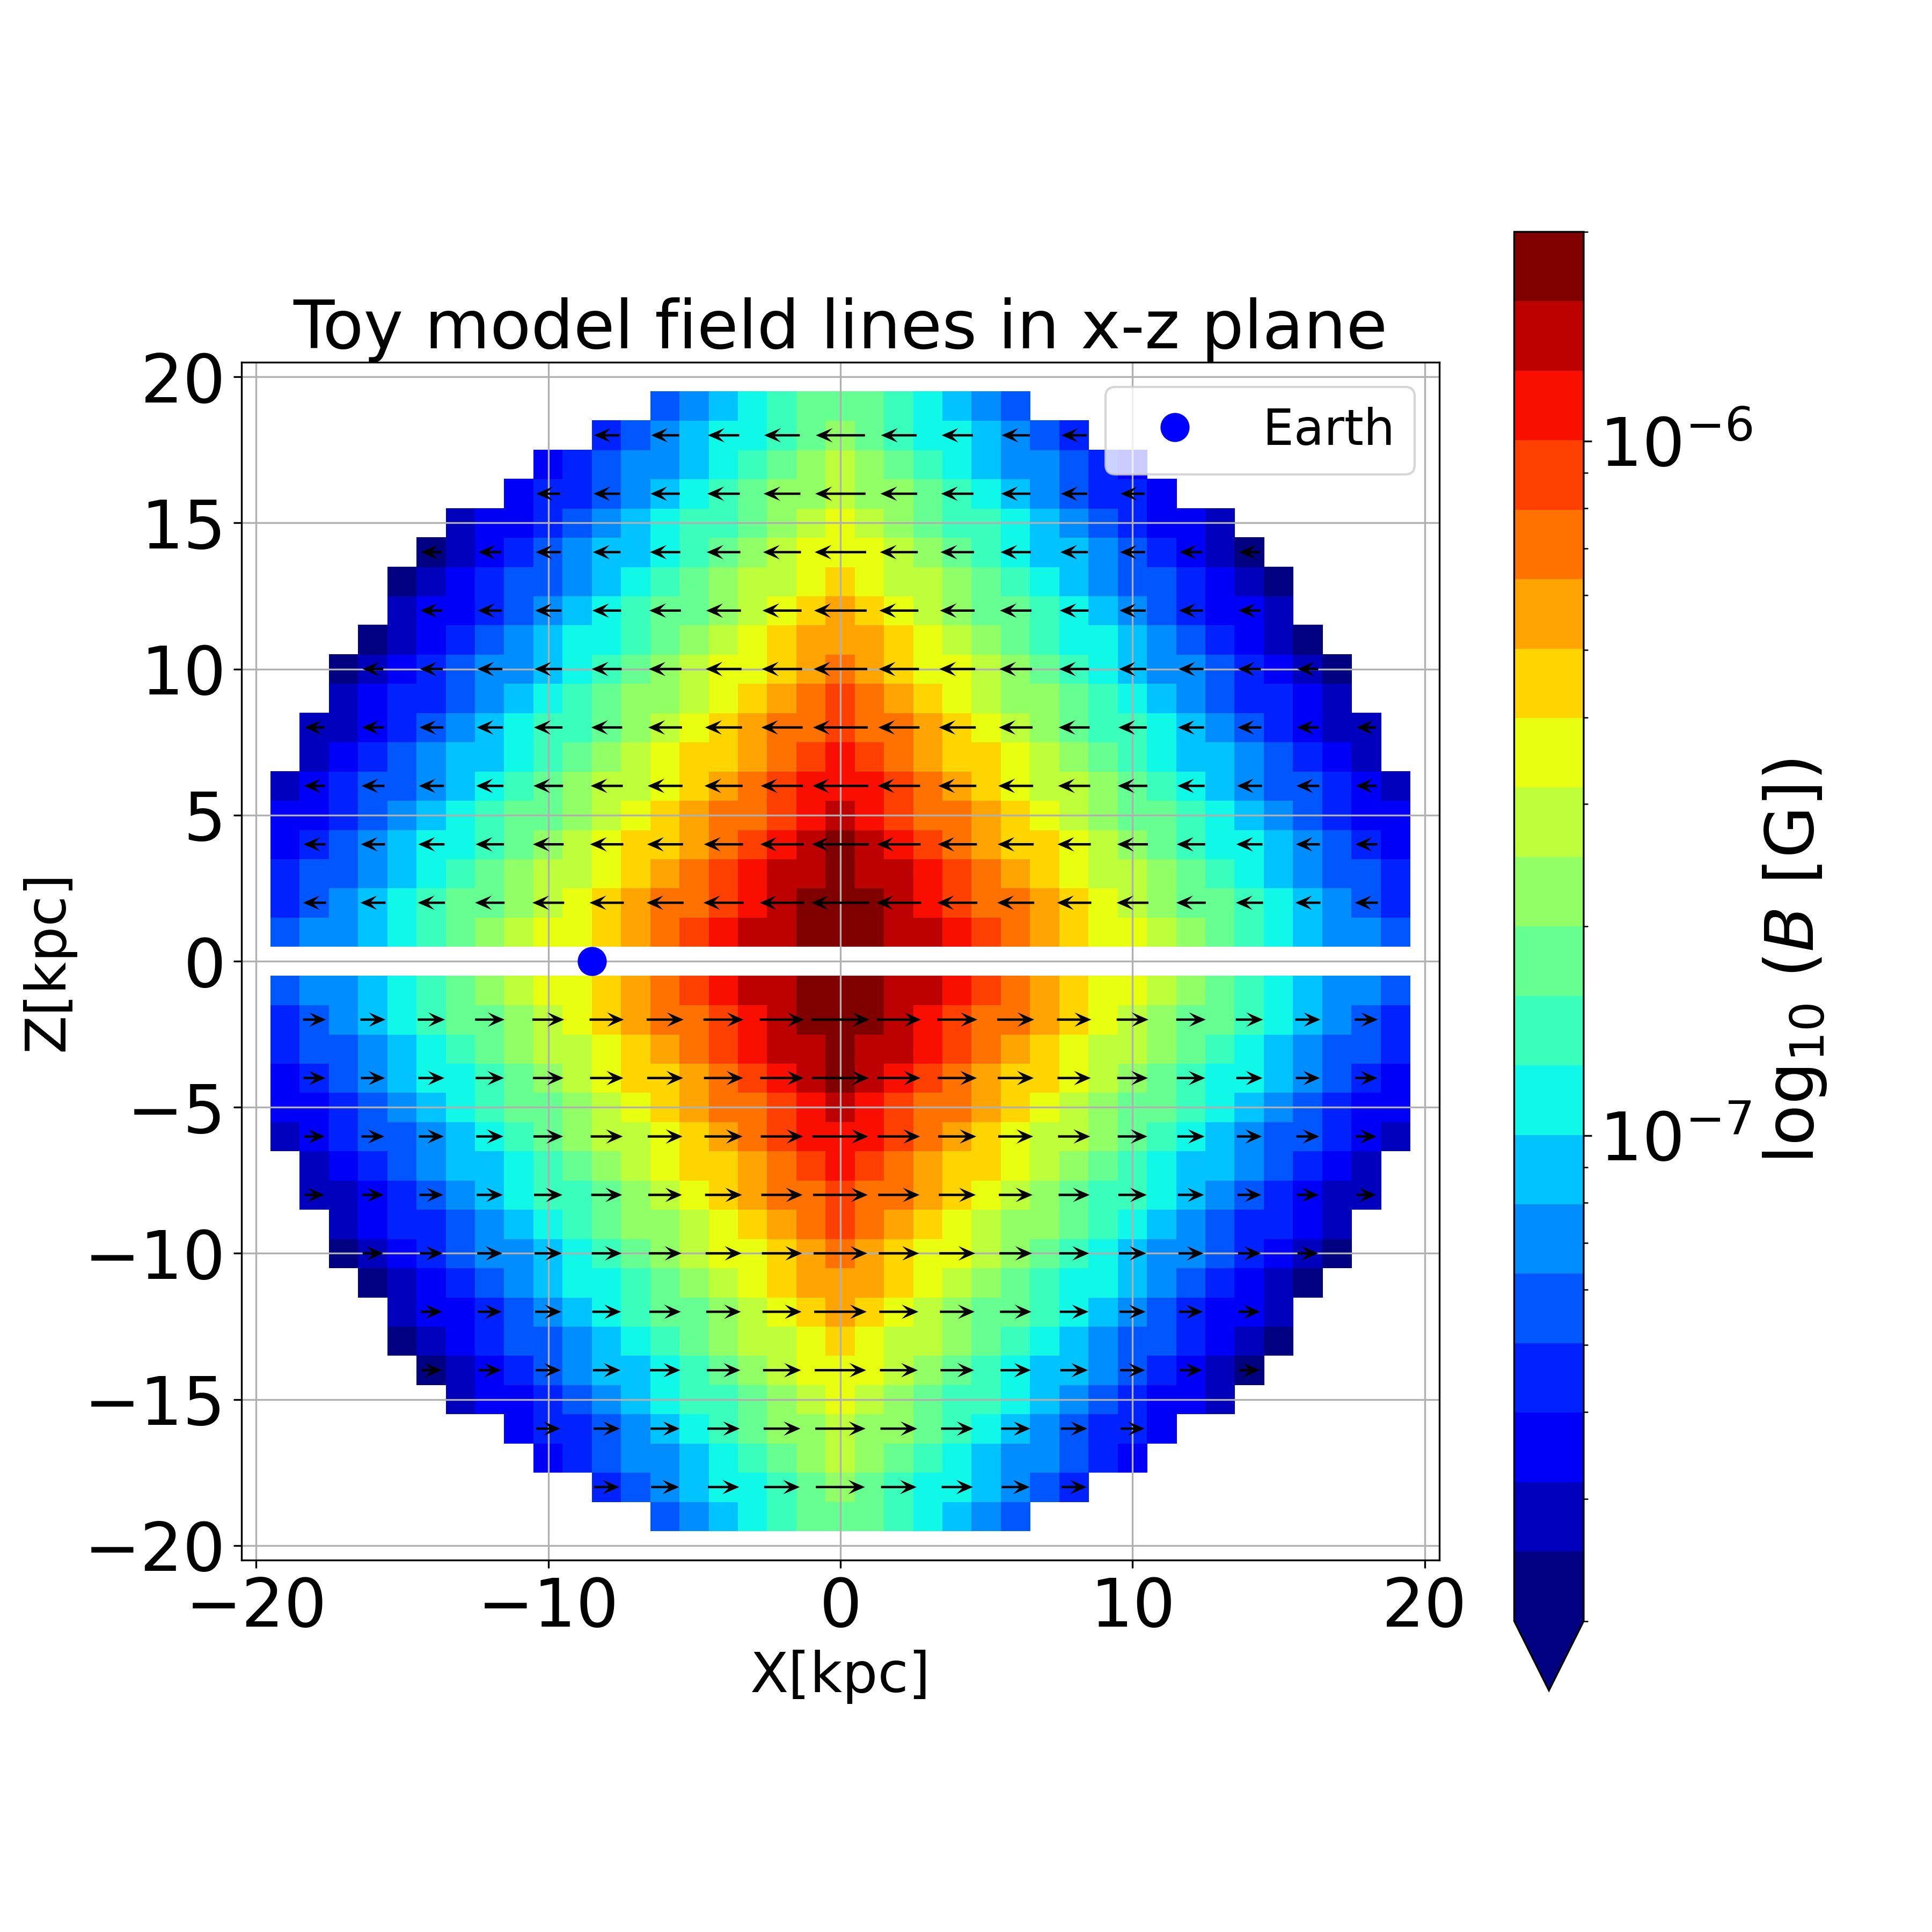
\includegraphics[width = 9cm]{Images/ToyModel_BestFit_XZ.png}%
    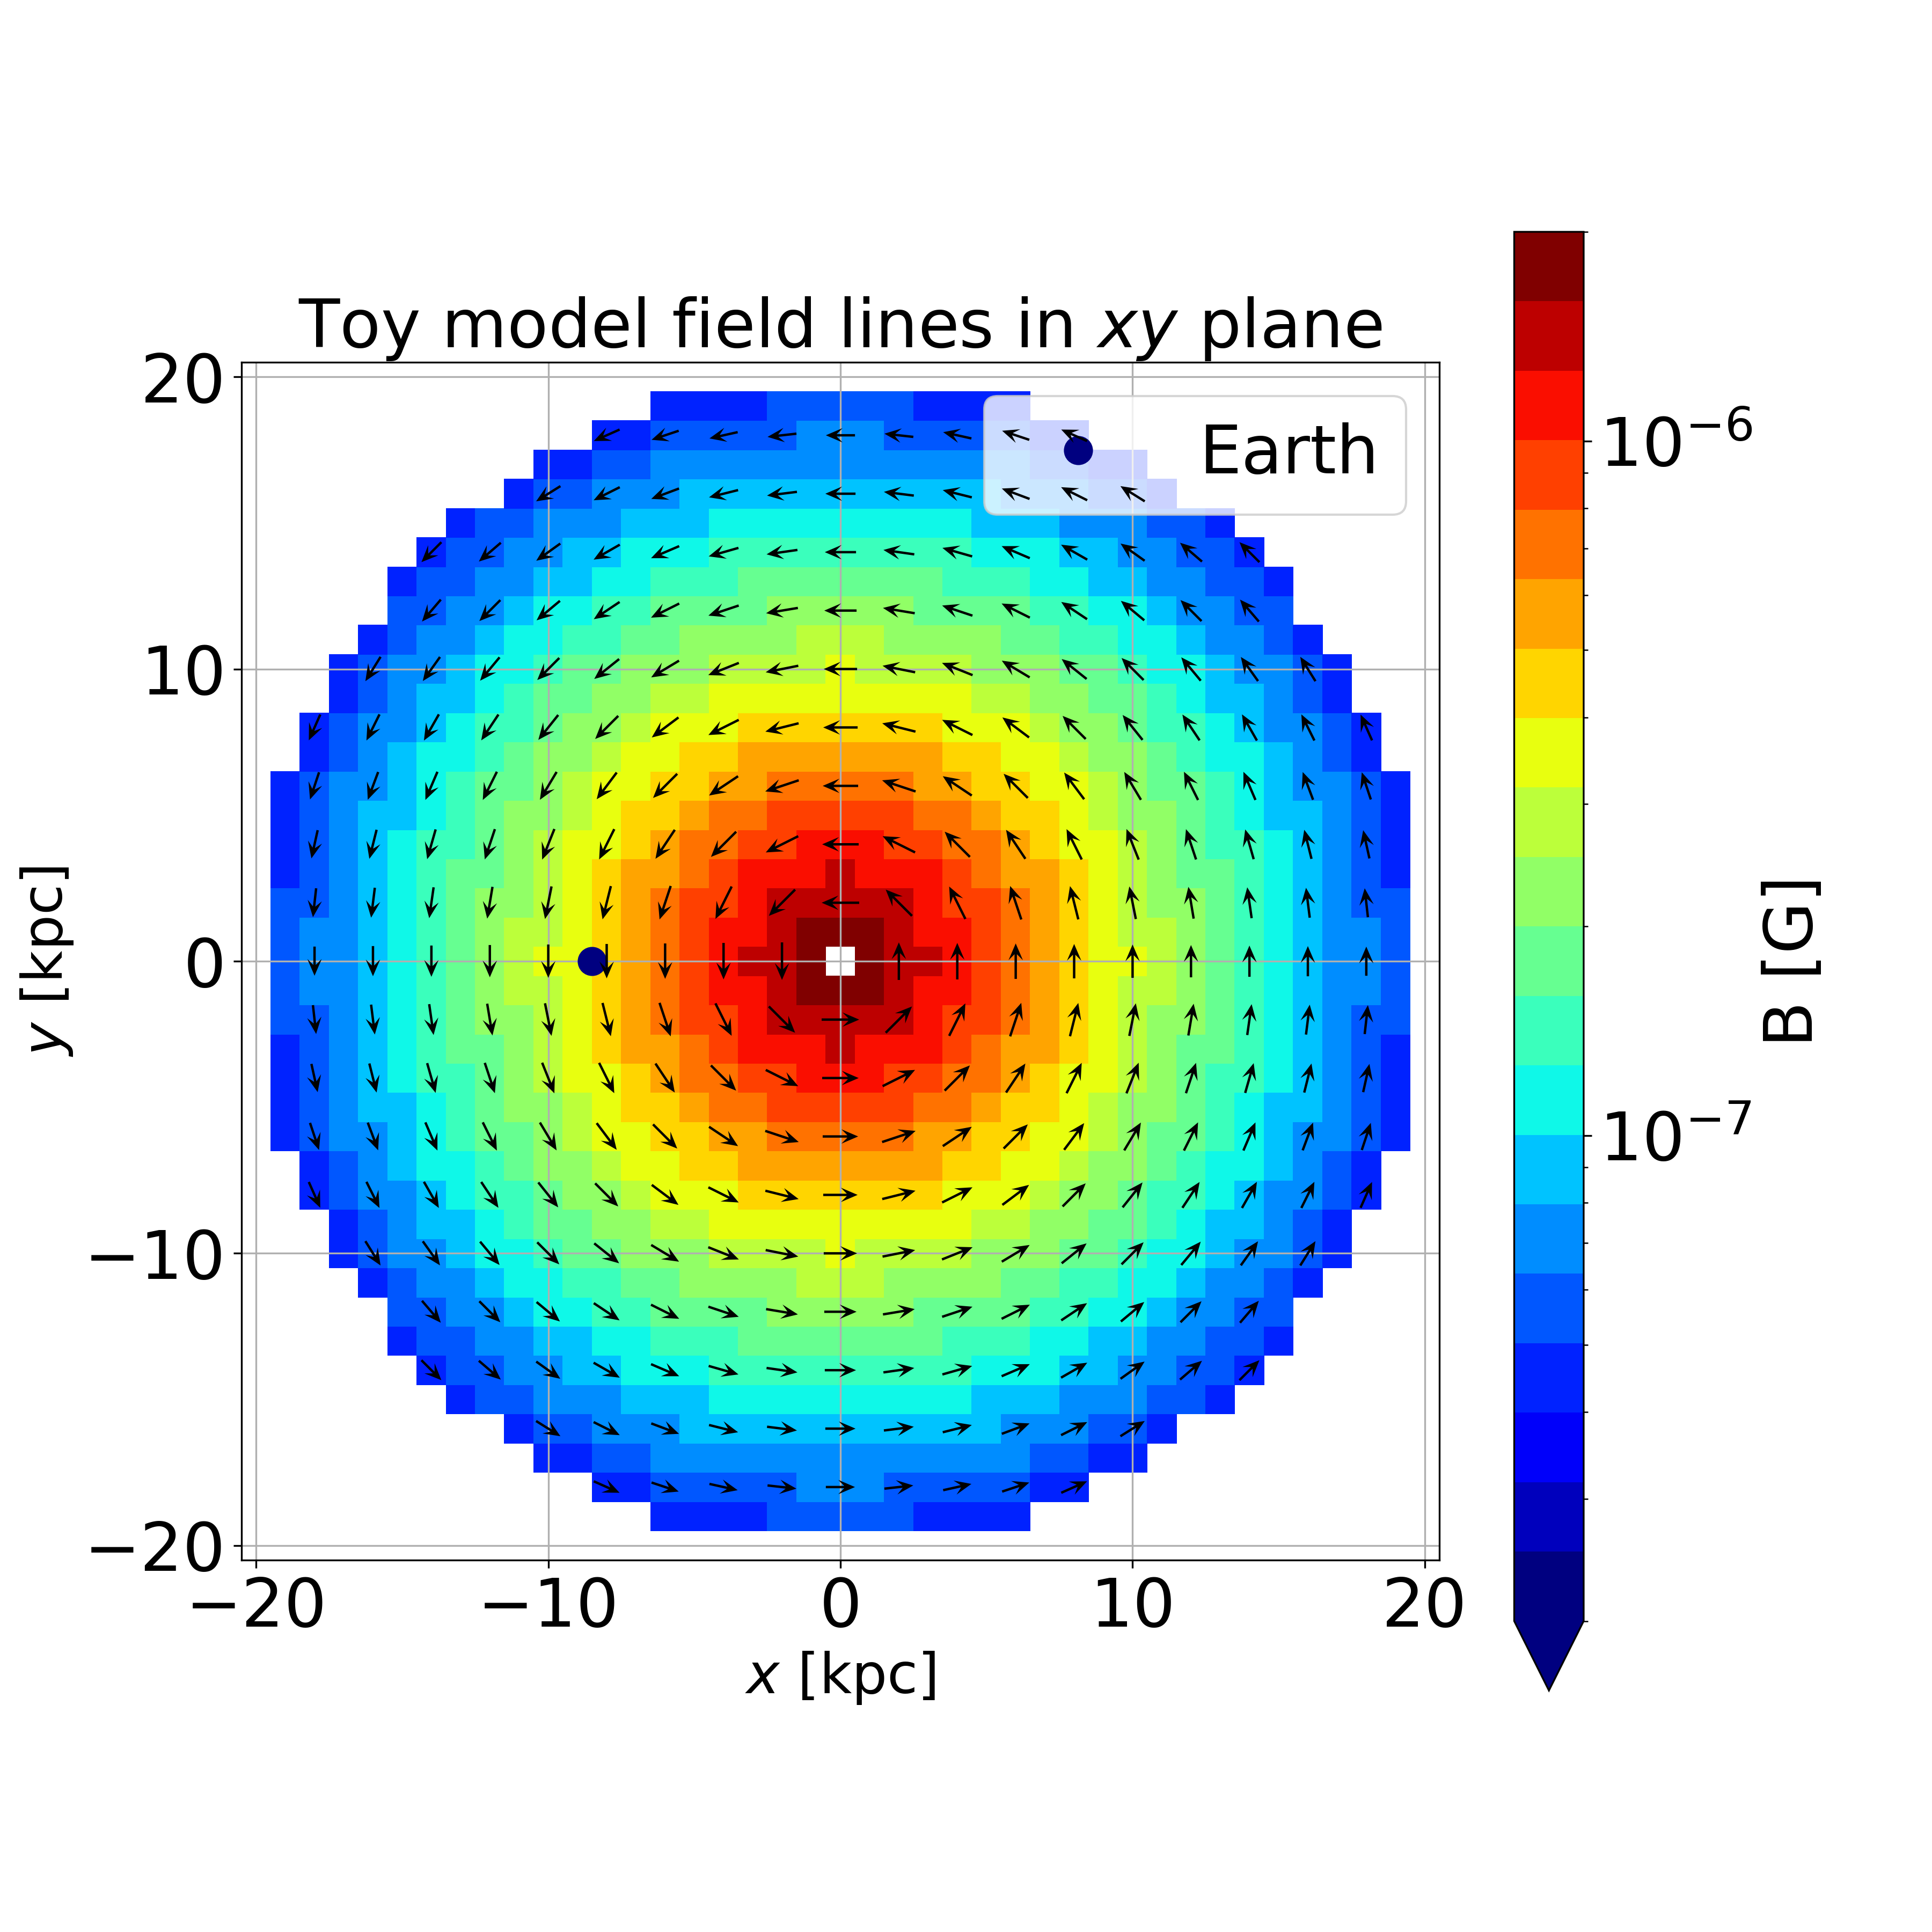
\includegraphics[width = 9cm
    ]{Images/ToyModel_BestFit_XY.png}
    \caption{Cross-section of toy model for the Galactic magnetic field in the Galactic halo region in the XY and XZ plane (with the Galactic plane in the XY plane at $z=0$) showing their drop in two dimensions.}
    \label{fig:Vis_TM}
\end{figure}
\clearpage

%Discuss the electron distribution
\subsubsection{Electron Distribution}

In order to produce synthetic synchrotron maps an electron distribution is required.
The JF12 model considered both the WMAP analytical expression \ref{Eq_WMAP_EdNdE}
and simulated electron distribution from GALPROP. They used the latter for their model in their paper.
The two models are quite different. The WMAP \cite{WMAP_Page} model is an analytical expression whereas the GALPROP \cite{Hammurabi} is based on numerical simulations and the distribution of supernova remnants in the Galaxy. For our toy model we adopted the WMAP distribution model. Our current knowledge of the non-thermal electron distribution in the Galaxy, especially in the Galactic halo region, is very limited. We therefore prefer to adopt a simple analytical model in order to avoid adding further layers of complexity. The WMAP electron distribution model is:
\begin{equation}\label{Eq_WMAP_EdNdE}
    \frac{\mathrm{d}N_e}{\mathrm{dlog}E_{e}} =     C_\mathrm{norm} \left(\frac{E_e}{\rm E_{\rm 10 GeV}}\right)^{-p+1} e^{-r/R_{\mathrm{el}}} \mathrm{sech}^2(z/Z_{\mathrm{el}}) 
\end{equation}
where $\frac{\mathrm{d}N_e}{\mathrm{dlog}E_{e}}$ is the differential electron density in a certain energy bins
in units of ${\rm cm}^{-3}$, $p =3$ is the spectral index. The parameters, $C_\mathrm{norm}$, describes the 10~GeV electron density, and $R_{\mathrm{el}}$ \& $Z_{\mathrm{el}}$ describe the radial and azimuthal spatial cut-offs. 


% EdNdE plots for some arbitrary parameters which will be fixed post equipartition scans.
\begin{figure}[h!]
    \centering
    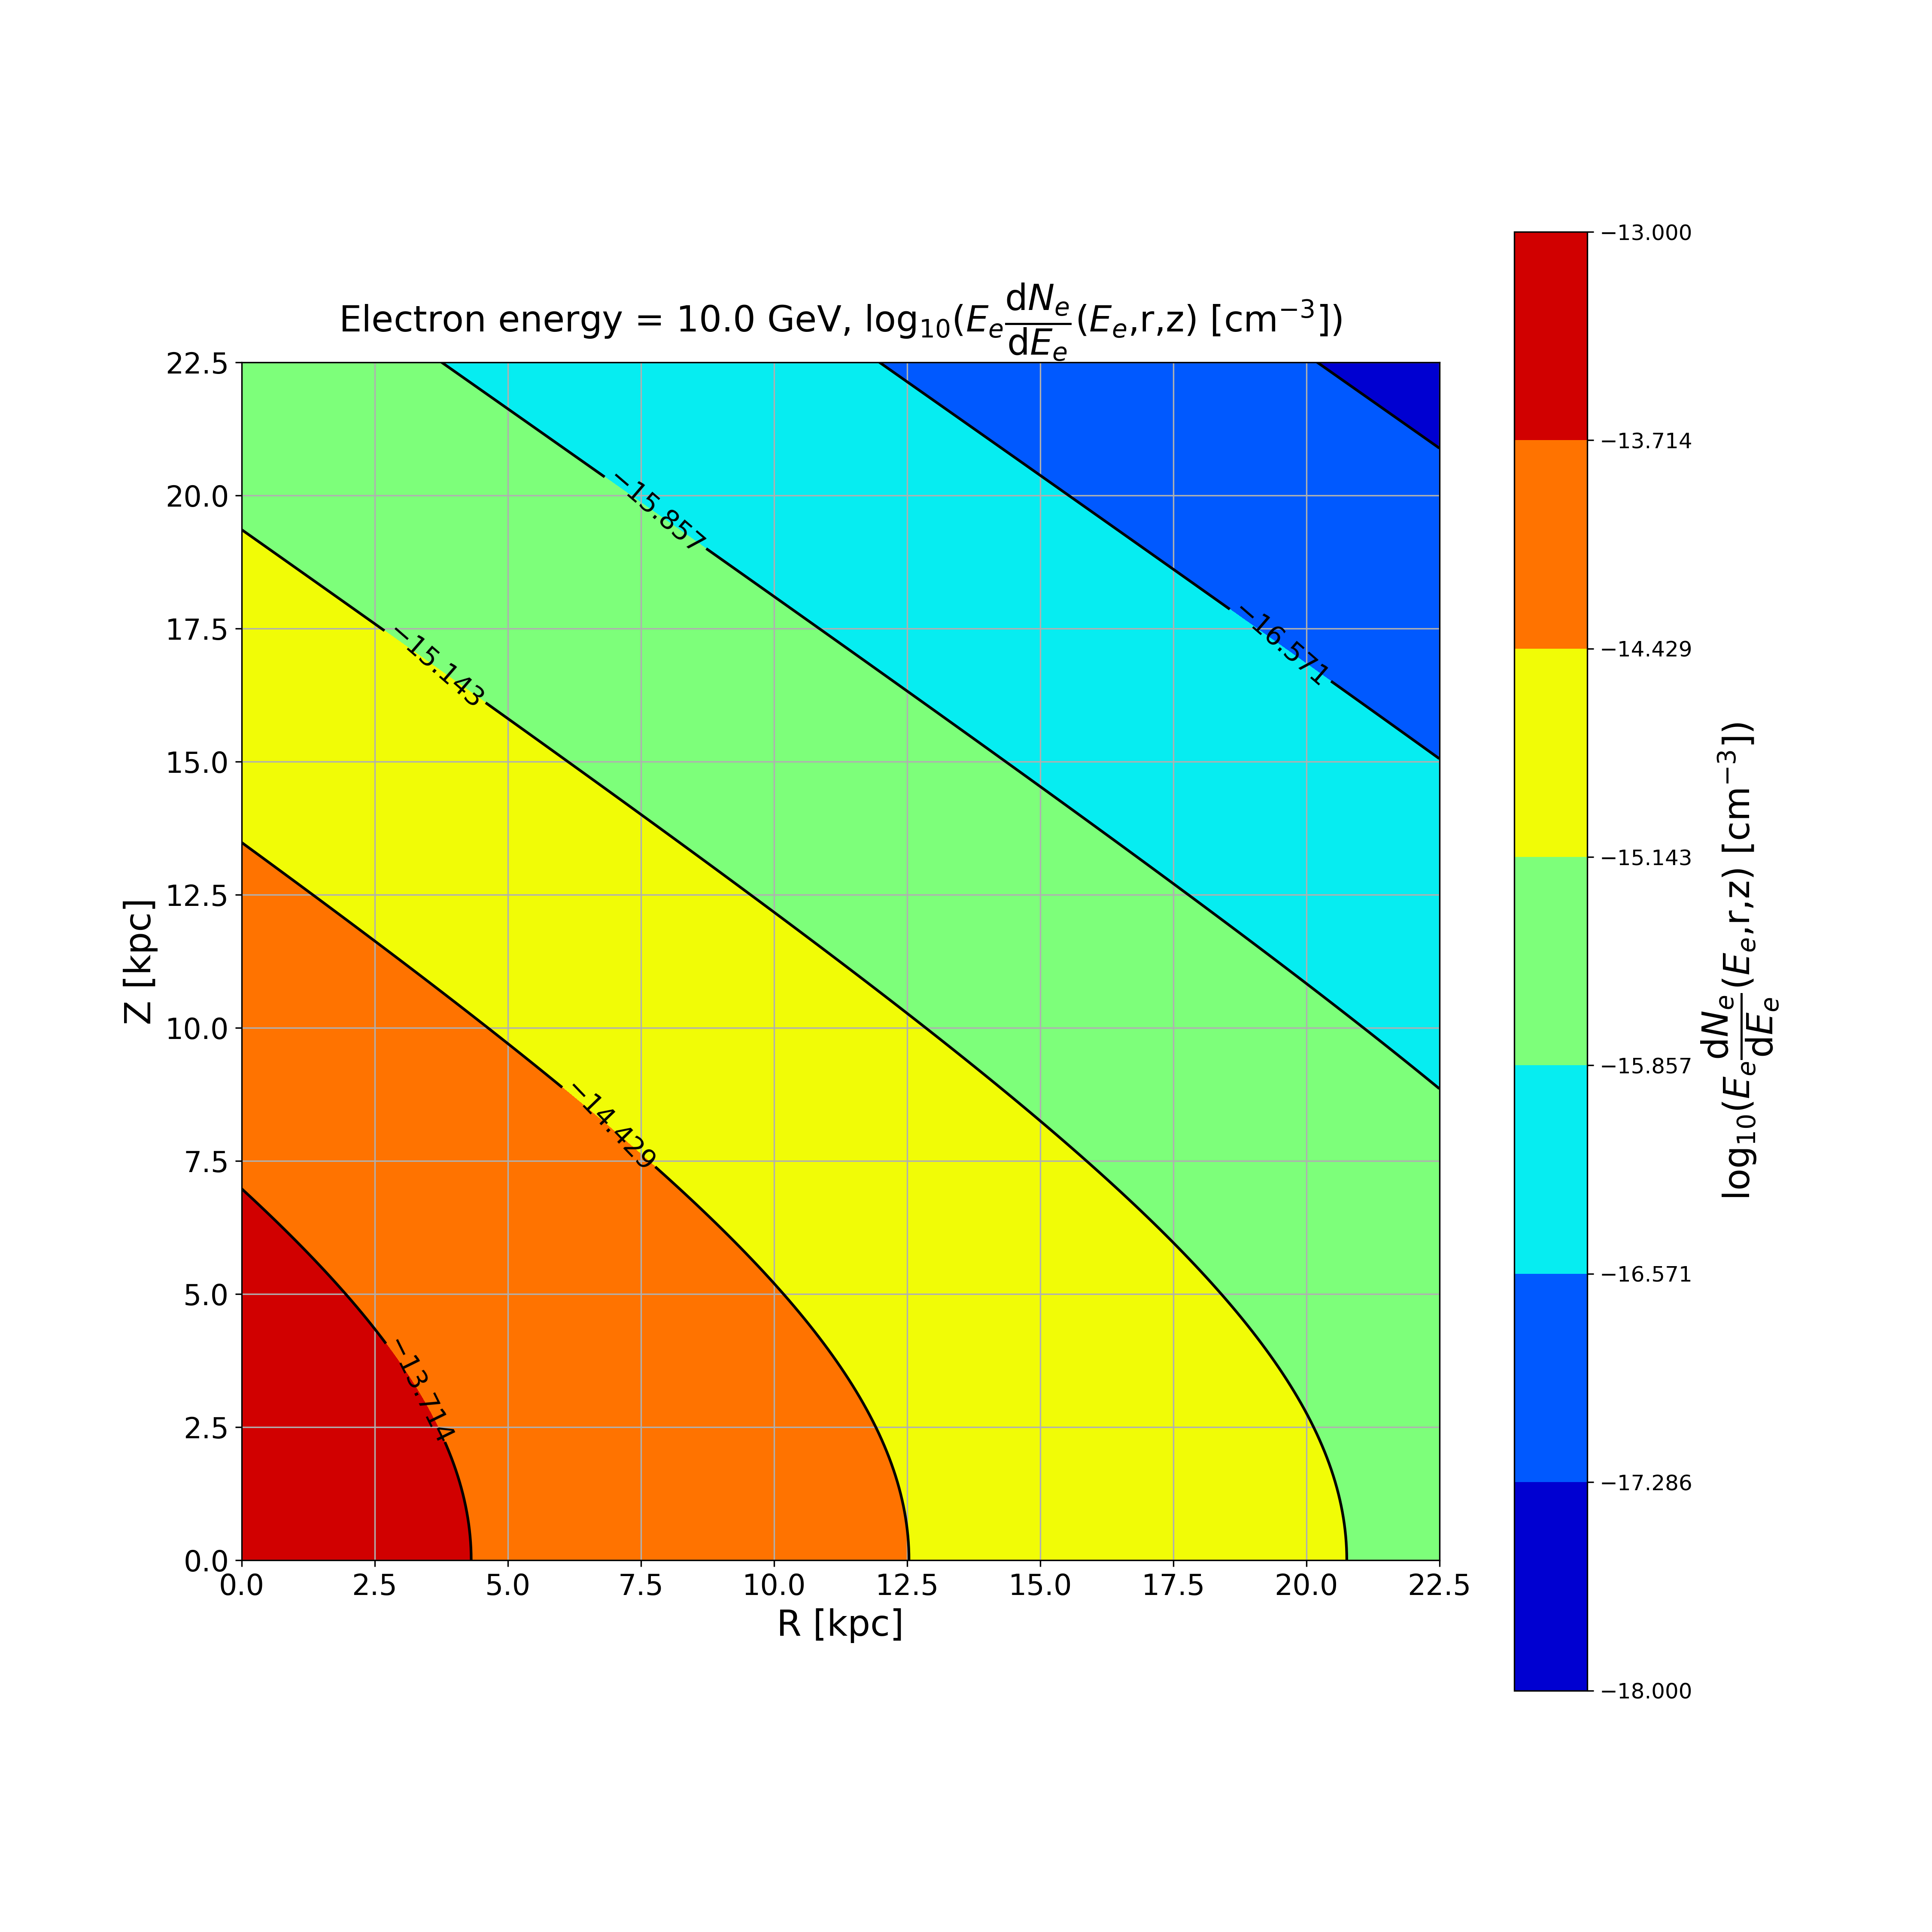
\includegraphics[width= 8cm]{Images/Linear_EdNdE.png}%
    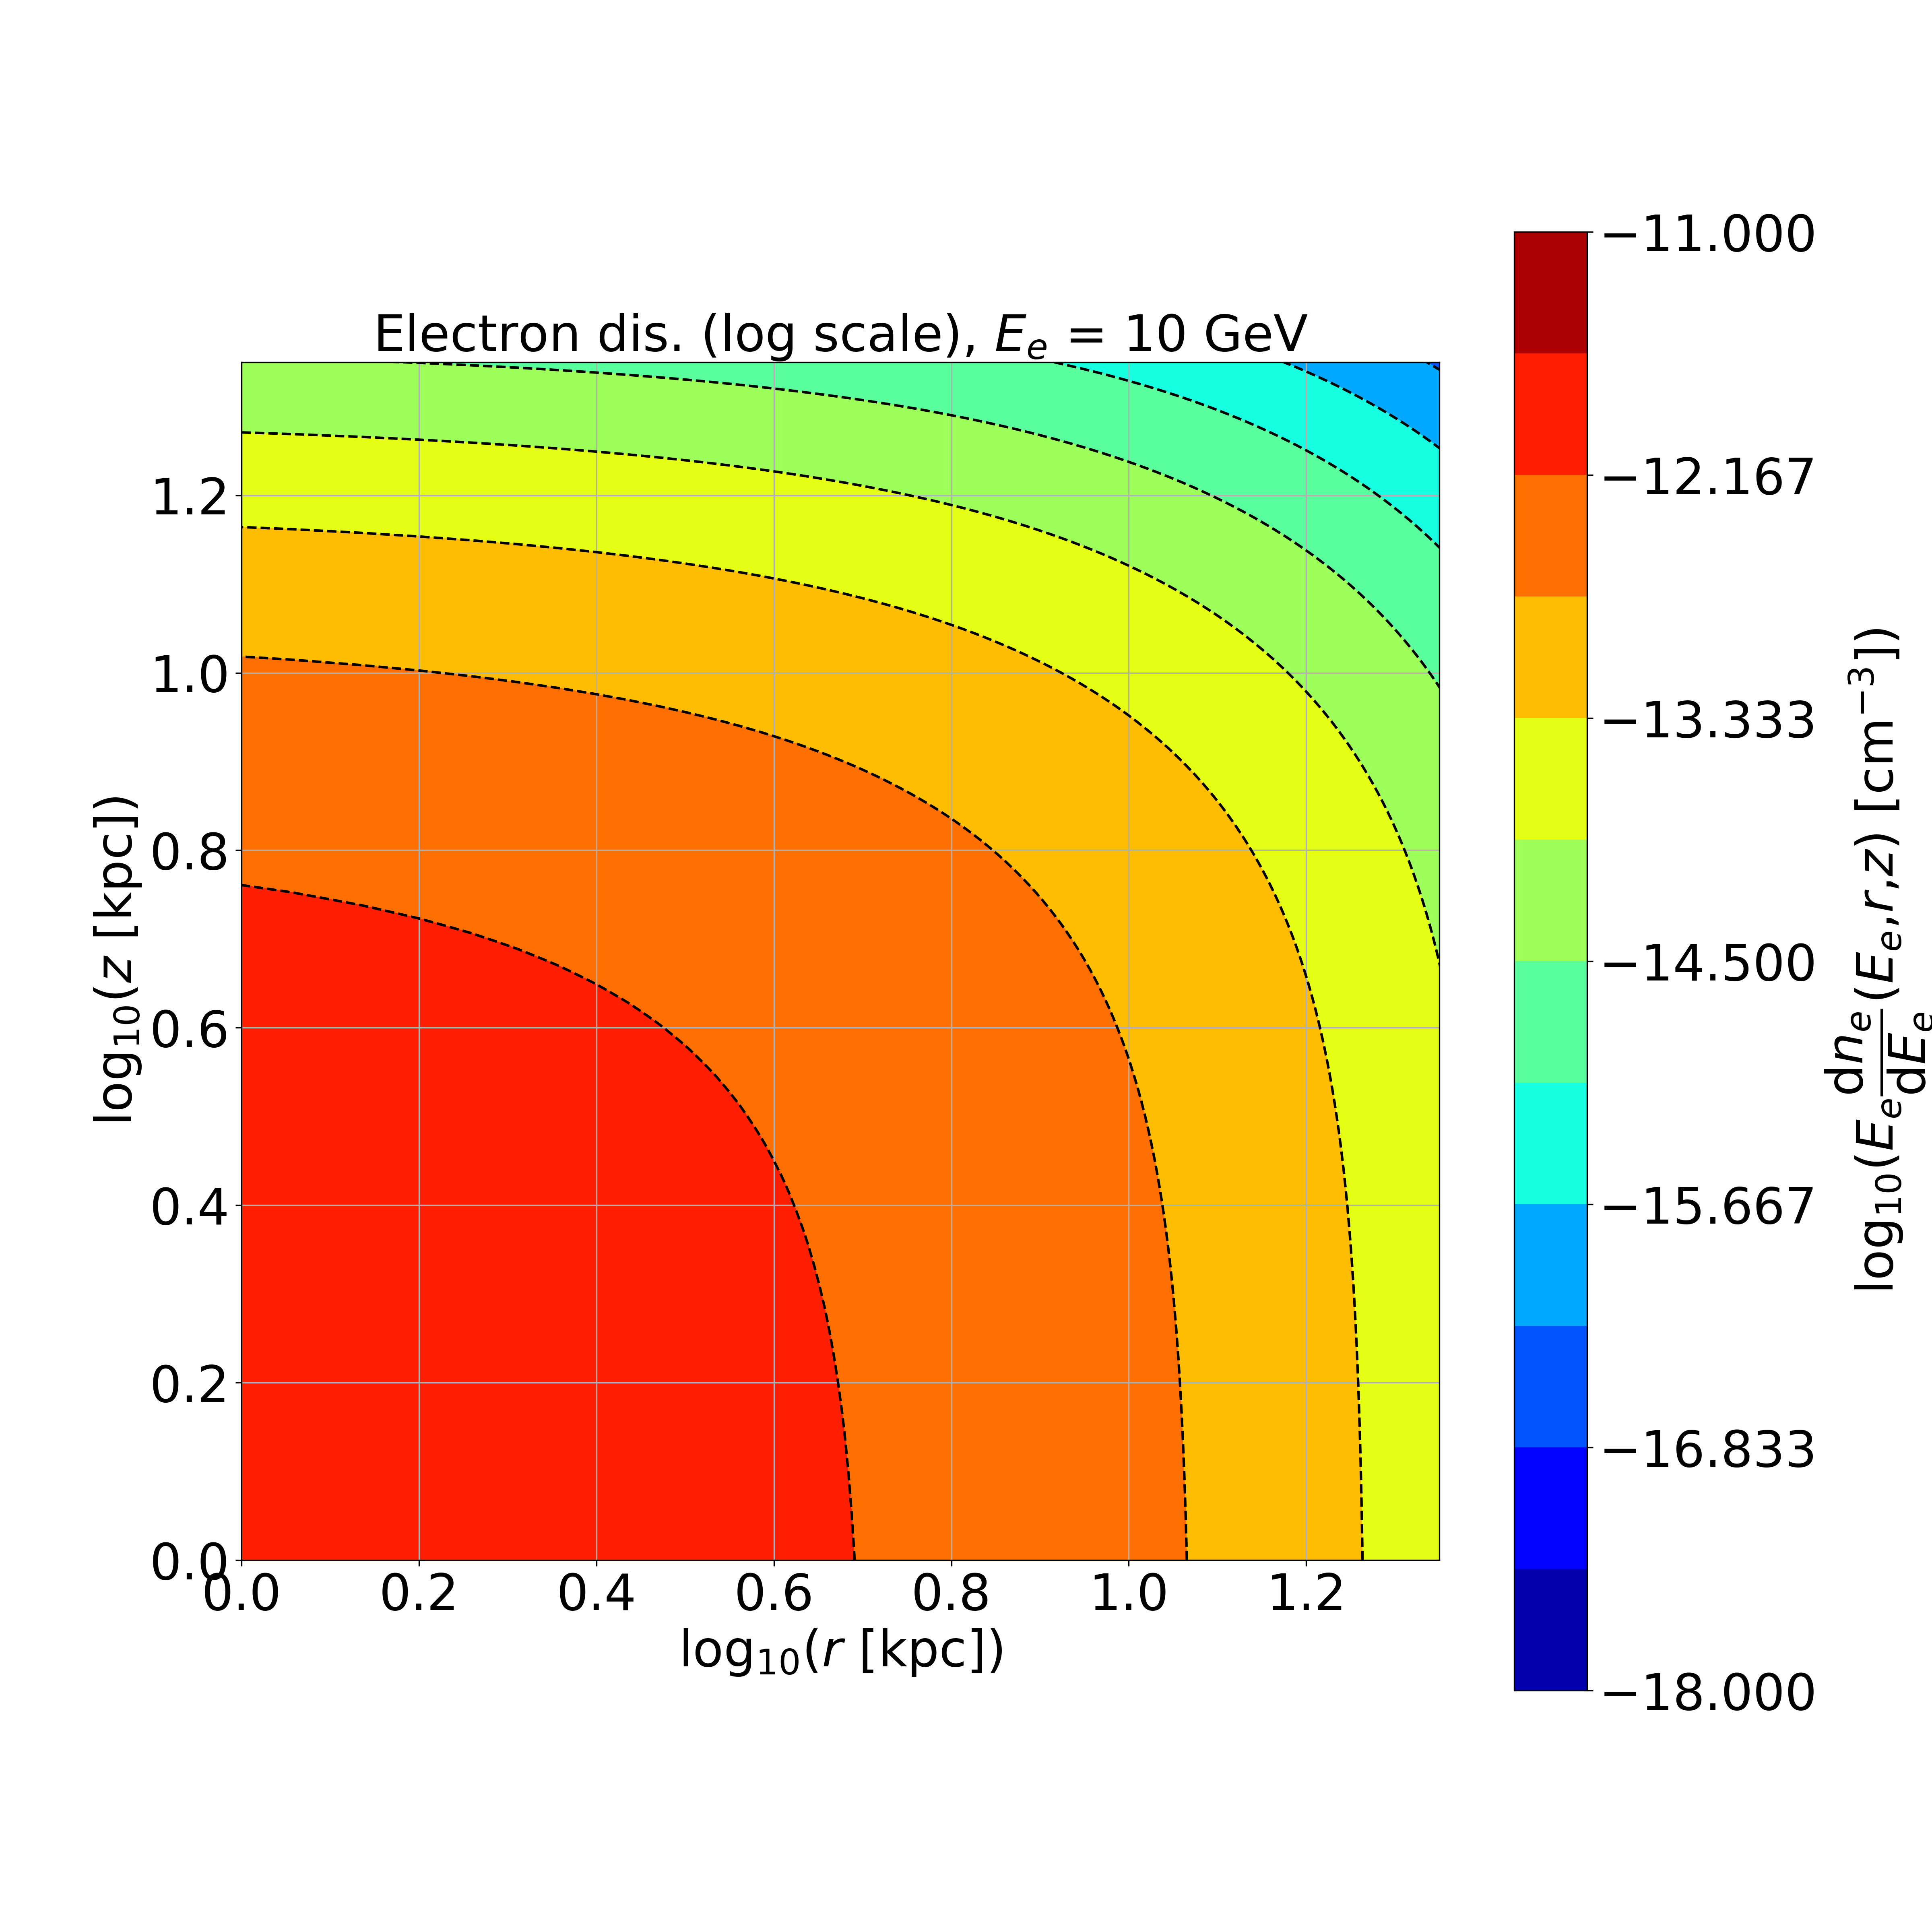
\includegraphics[width = 8cm]{Images/Log_EdNdE.png}
    \caption{Electron distribution for $R_{\mathrm{el}} = 5$ kpc and $Z_{\mathrm{el}} = 7$~kpc in linear scale on left and log-scale on right.}
    \label{fig:my_label}
\end{figure}

% synchrotron radiation expressions and theory, also the appendix.
\subsection{Synchrotron Emission}\label{Synchrotron_theory}

\subsubsection{Intensity \& polarisation}
Synchrotron radiation or magneto-bremsstrahlung radiation is the radiation produced due to charged particles that gyrate at relativistic speeds around a static magnetic field. The radiation produced via synchrotron is often linearly polarised.
%The radiation received from a single particle is elliptically polarised and the sense of polarisation (right or left handed) is determined by whether the line of sight sits inside or outside the cone of radiation.
%However, for a distribution of particles that vary smoothly with the pitch angle, the elliptical component cancels out and so the emission cones will contribute equally on each side of the line of sight. The radiation then is linearly polarised. 
The polarised emission can be visualised as an ellipse where the major axis is the perpendicular component ($J_{\rm \perp}$) and the minor axis is the parallel ($J_{\parallel}$) component. We provide a detailed explanation of this in appendix~(\ref{Appendix_A}). 

Equations \ref{Jperp} and \ref{Jpara} describe the two polarised components $J_{\perp}$ and $J_{\parallel}$ for a  given peak photon energy $E_{\gamma}^{\mathrm{peak}}$. In this case, $E_{\gamma}^{\mathrm{peak}} = 1.175 \times 10^{-4}$~eV which is corresponding 28.4~GHz, the peak frequency for 30~GHz Planck data.
\begin{equation}\label{Jperp}
 {J_{\perp}^l} =   \int_{\mathrm{log}E_e^{\mathrm{min}}}^{\mathrm{log}E_e^{\mathrm{max}}}\mathrm{dlog}E_{e} \  \frac{\mathrm{d}N_e}{\mathrm{dlog}E_{e}} \  \left[F\left(\frac{E_{\gamma}}{E_{\gamma}^{\mathrm{peak}}}\right) + G\left(\frac{E_{\gamma}}{E_{\gamma}^{\mathrm{peak}}}\right)\right] * \frac{B_{\perp}}{B_{\mathrm{crit}}}\frac{m_{e}}{h} \frac{8\pi \alpha}{9} 
\end{equation}

and,

\begin{equation}\label{Jpara}
{J_{\parallel}^l} = \int_{\mathrm{log}E_e^{\mathrm{min}}}^{\mathrm{log}E_e^{\mathrm{max}}}\mathrm{dlog}E_{e} \ \frac{\mathrm{d}N_e}{\mathrm{dlog}E_{e}} \  \left[F\left(\frac{E_{\gamma}}{E_{\gamma}^{\mathrm{peak}}}\right) - G\left(\frac{E_{\gamma}}{E_{\gamma}^{\mathrm{peak}}}\right)\right] * \frac{B_{\perp}}{B_{\mathrm{crit}}}\frac{m_{e}}{h} \frac{8\pi \alpha}{9}
\end{equation}
where the functions,
\begin{align}
F(x) &= x \int_x^\infty K_{5/3}(x') dx'\\
G(x) &= x K_{2/3}.
\end{align}
These expressions are provided in terms of the critical field magnetic field strength, $B_{\mathrm{crit}} \frac{m_e^2c^3}{e\hbar} = 4.414 \times 10^{13}$~G, where $m_e = 0.511$~MeV is the mass of electron, $h = 4.136 \times 10^{-15}$~eV-sec is the Planck's constant and $\alpha \approx \frac{1}{137.04}$ is the electromagnetic fine structure constant.

For clarity, several of the conventions we adopted are here noted. The parallel component of polarisation (${J_{\parallel}}$) is orientated in the same direction as  $\vec{B_{\perp}}$, and the perpendicular component of polarisation (${J_{\perp}}$) is perpendicular to $\vec{B_{\perp}}$. The Stokes parameters at each point along the line of sight can be written in terms of the intrinsic polarisation angle $\Psi^l_{\rm in}$ which is the angle between the line of sight perpendicular component of the magnetic field $B_{\perp}$ and Galactic south at each step. The conventions adopted here match those used by the Planck collaboration \cite{Planck_XIX} based on the $\rm HEALPix^3$~\footnote{\textcolor{purple}{https://healpix.jpl.nasa.gov/}} software by \cite{Healpix_2005}. For each step along the line-of-sight, both  ${J_{\perp}^l}$ and ${J_{\parallel}^l}$ are subsequently used to obtain the $Q$ and $U$ Stokes parameters. The integrated values along the line of sight can be defined as  $Q^{\rm tot}_{\rm in}$ and $U^{\rm tot}_{\rm in}$ as:
\begin{eqnarray}
Q_{\rm in}^{\rm tot} = {\int_0^L \mathrm{d}l \ ({J_{\perp}^l} - J_{\parallel}^l) \ {\cos}(2\Psi^l_{\rm in}) } \\
U_{\rm in}^{\rm tot} = {\int_0^L \mathrm{d}l \ ({J_{\perp}^l} - J_{\parallel}^l) \ {\sin}(2\Psi^l_{\rm in})} \,
\end{eqnarray}


The polarised flux ($I_{\rm pol}$) can then be expressed in terms of the intrinsic Stokes parameters which are integrated along the line of sight (${Q_{\rm in}}$ \& ${U_{\rm in}}$) :
\begin{eqnarray} \label{eq_I_pol}
I_{\rm pol} = \sqrt{(Q_{\rm in}^{\rm tot})^2+(U_{\rm in}^{\rm tot})^2} = J_{\perp}^{\rm tot} - J_{\parallel}^{\rm tot} ,\ \rm and
\end{eqnarray}
\begin{equation} \label{eq_I_tot}
    I_{\rm tot} = J_{\perp}^{\rm tot} + J_{\parallel}^{\rm tot} 
\end{equation}
$J_{\perp}^{\rm tot}$ and $J_{\parallel}^{\rm tot}$ are the resultant magnitudes of emissions in perpendicular and parallel directions and can be given by:
\begin{eqnarray}
J_{\perp}^{\rm tot} = (I_{\rm tot} + I_{\rm pol})/2 \\
J_{\parallel}^{\rm tot} = (I_{\rm tot} - I_{\rm pol})/2 
\end{eqnarray}
In appendix(\ref{Appendix_A}) we explain in detail the relation between these equations with two simplified cases.
The intrinsic polarisation angle $\Psi_{\rm in}$ between the Galactic south and the local magnetic field component perpendicular to the line of sight can be defined as:
\begin{eqnarray}
\tan(2\Psi_{\rm in}) = \frac{U_{\rm in}^{\rm tot}}{Q_{\rm in}^{\rm tot}} 
\end{eqnarray}

% Describe the Planck data set and what radio bands were used.

\subsection{Observational Data}
% discussion of data sets used
For our synchrotron emission study We use the publicly available from the Planck satellite mission \footnote{\textcolor{purple}{http://pla.esac.esa.int/pla/}}. Specifically, we use the polarised radio data at 30~GHz from Planck where the peak frequency is at 28.4~GHz, with a band width of 9.8~GHz. At this frequency a considerable level of polarised synchrotron emission is observed, with a only a small level of Faraday rotation occurring at these high frequencies. However, we also note that in this 30~GHz band, the Planck data cannot be used to probe synchrotron intensity directly, since at this frequency the unpolarised sky receives a considerable contributions from both thermal bremsstrahlung and anomalous microwave emission, as well as synchrotron radiation \Andrew{reference needed to justify this claim}. 
%\Andrew{justification of Planck bands not considered needs providing}
%We intentionally do not consider the low frequency data available from S-PASS, since this data set masks out a large region of the Galactic halo bubbles and would not prove suitable for our study. \Andrew{mentioning data sets not used looks odd here}

%(see section \ref{Faraday_Rotation}). 
% Hence, we also do a comparison with the 408~MHz Haslam data for total intensity where most of the unpolarised radiation comes from the synchrotron radiation.
%\textcolor{blue}{Results} section.

%\clearpage
%\newpage
%\subsection{Comparison to Planck data}
\section{Results}
\label{Results}

%\Vasu{I have added the points to address in the result section.}
%% Skymap comparison and explanation of smoothening method



Utilising the setup described in the previous section (see section~\ref{Methods}), we generate a synthetic polarised synchrotron emission map for each parameter set of our toy model. The toy model comprises of 5 free parameters, (see table~\ref{Para_table}). The radial cut-off of the magnetic field and electron distribution is kept identical $R_{\mathrm{Mag}}$ = $R_{\mathrm{el}}$ and the same applies to the azimuthal cut-off $Z_{\mathrm{Mag}}$ = $Z_{\mathrm{el}}$. The reason for this constraint is that synchrotron radiation level depends on both non-thermal electron density and magnetic field strength. Thus, even if the spatial extend of the magnetic field differs from the electron distribution, one can only probe the field in the region where both the field and electrons are present. The minimum and maximum value for the spatial parameters are 2~kpc to 19~kpc, which are scanned over in step size of 1~kpc. 
The range over which both $B_{\rm str}$ and $B_{\rm tur}$ are scanned is 2$~\mu$G to 19$~\mu$G, with a step size of 1$~\mu$G. We calculate the polarised emission for one particular value of $\log_{10}(C_{\rm norm}[{\rm cm}^{-3}]) = -13.85$, and subsequently re-scale these results to obtain the polarised emission maps for different values of  $\log_{10}(C_{\rm norm} [{\rm cm}^{-3}])$, ranging this scan from $-10$ to $-15$ with a step size of $0.25$ (ie. in 20 steps).


%\Vasu{I have addressed this.}We use the techniques \Andrew{techniques? synchrotron emission methods you mean?} mentioned in Section~\ref{method} to generate synthetic polarised synchrotron radiation skymaps. 

In our study, we mask out three regions from our skymaps. The first of these is in the Galactic disc region between b = $(-15^{\circ},15^{\circ})$. For the second region, based on observations from \cite{eROSITA} and \cite{Su_2010}, we block out longitudes  $\geq \pm 90^{\circ}$ from the Galactic center (ie. all direction pointing away from the Galactic center direction), so as to ensure that our analysis only covers the region occupied by the Galactic Halo (Fermi and eRosita) bubbles. Lastly, we block out the region associated with the North Polar Spur (NPS). Our motivation here is that the higher latitudes of NPS seem to follow a trend to be originating locally rather than from Galactic center based on the starlight polarisation observations \cite{Gina_2021}. In order to remain as impartial as possible for the designation of this region, we adopt a cut for it selected in \cite{Wolleben_2007}. In fig.~\ref{fig:Skymaps} observational and synthetic skymaps are shown with these three regions removed.

To obtain best-fit for our model we ran a grid search for over a million configurations. For each toy configuration, a synthetic skymap was generated using Healpix \cite{Healpix_2005}, adopting a resolution with Nside = 32. Since the interests of our study are focused on large scale structures, both the synthetic skymaps and observational data were smoothed out, using a Gaussian kernel, on size scale of $15^{\circ}$, to wash out smaller scale features. We then compare the simulated polarised emission with the Planck data at 30~GHz by evaluating the $\chi^{2}$ value of the model fit to the data. To find the best fit parameters and their constraints, we carry out a grid search over the 5 free parameters, sampling in total a million parameter points.%We convert the temperature units ($K_{\rm CMB})$ of Planck data into brightness units (cm$^{-2}$~sec$^{-1}$~sr$^{-1}$). THIS IS OBVIOUS


In Fig.~\ref{fig:Skymaps} the smoothened skymap obtained from the best fit value of the parameters and the smoothened polarised Planck data is shown along with the residuals. The best-fit values used for the parameters are provided in table~\ref{Para_table}. 
%% Polarisation fraction
We next estimate the polarisation fraction obtained by our best-fit toy-model which is given in figure \ref{fig:Skymaps} which was calculated taking the ratio of the polarised to the total intensity. The polarisation fraction for the best-fit toy model is comparable to the values as seen in the observation data \cite{Carretti_2013} and \cite{WMAP_Page}.
%% Polarised Skymap

\begin{figure}[h!]
        \centering
        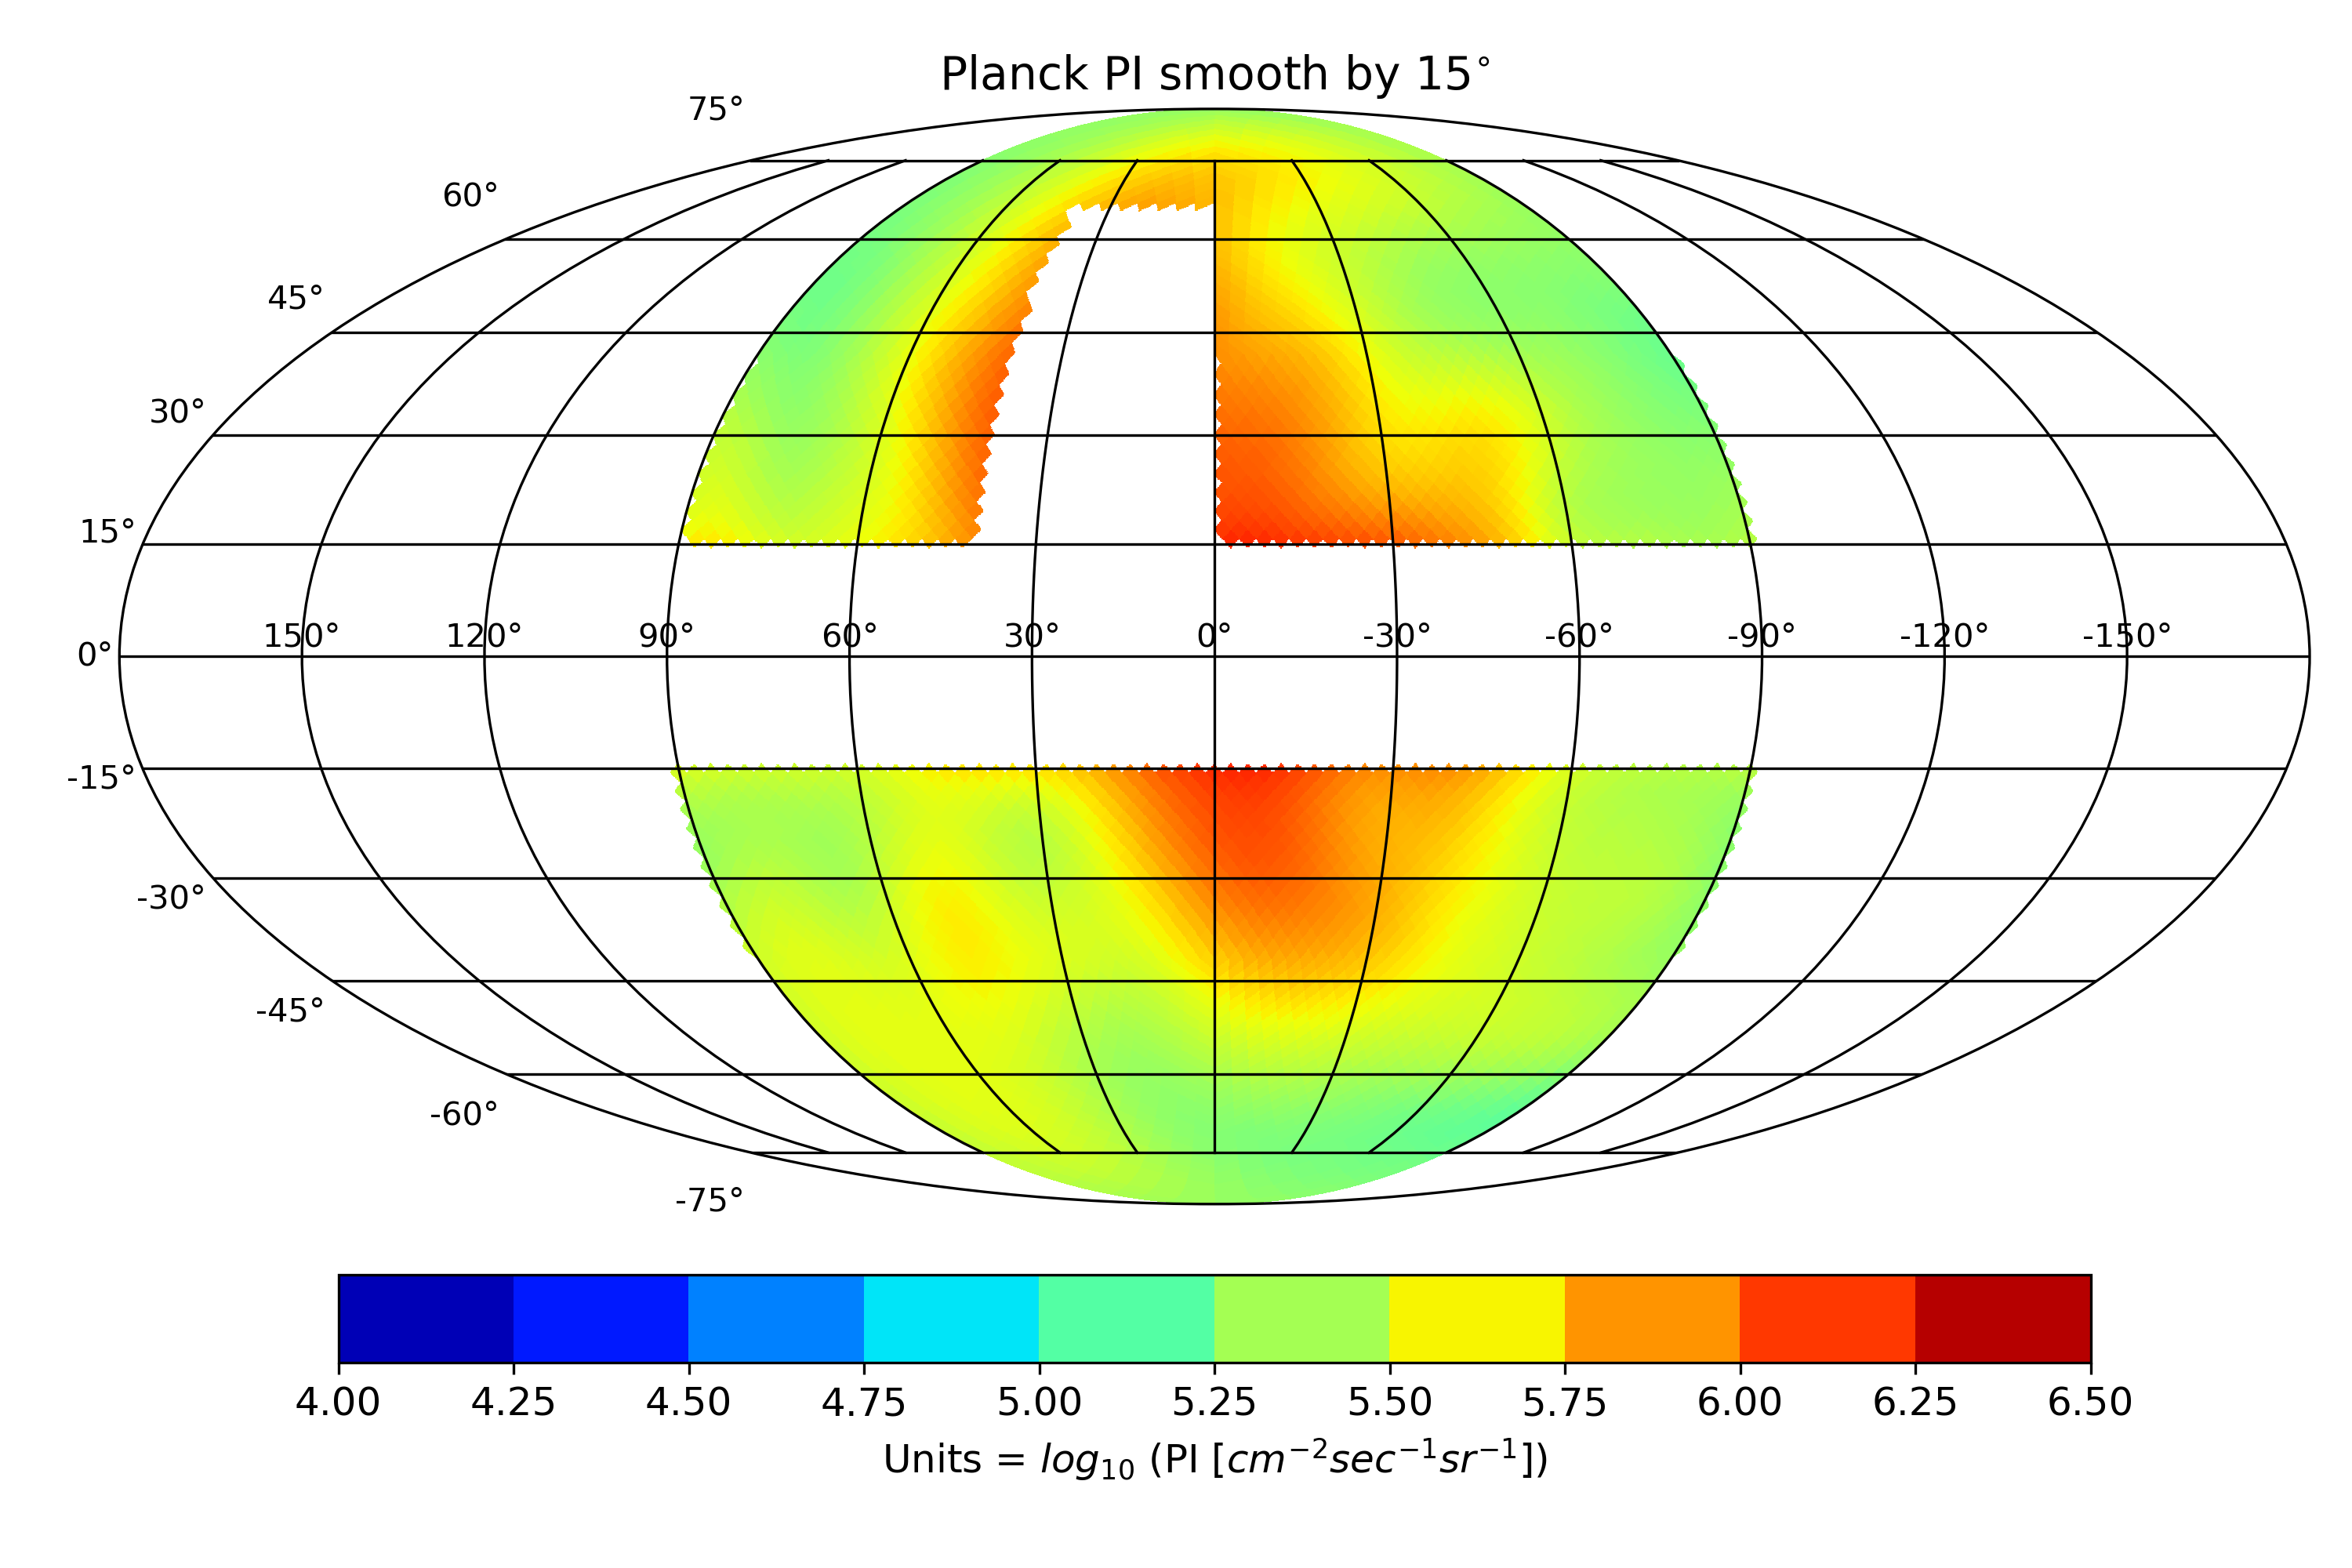
\includegraphics[width =9cm]{Images/Jan-17-2022_Planck_Sky_Map.png}%
        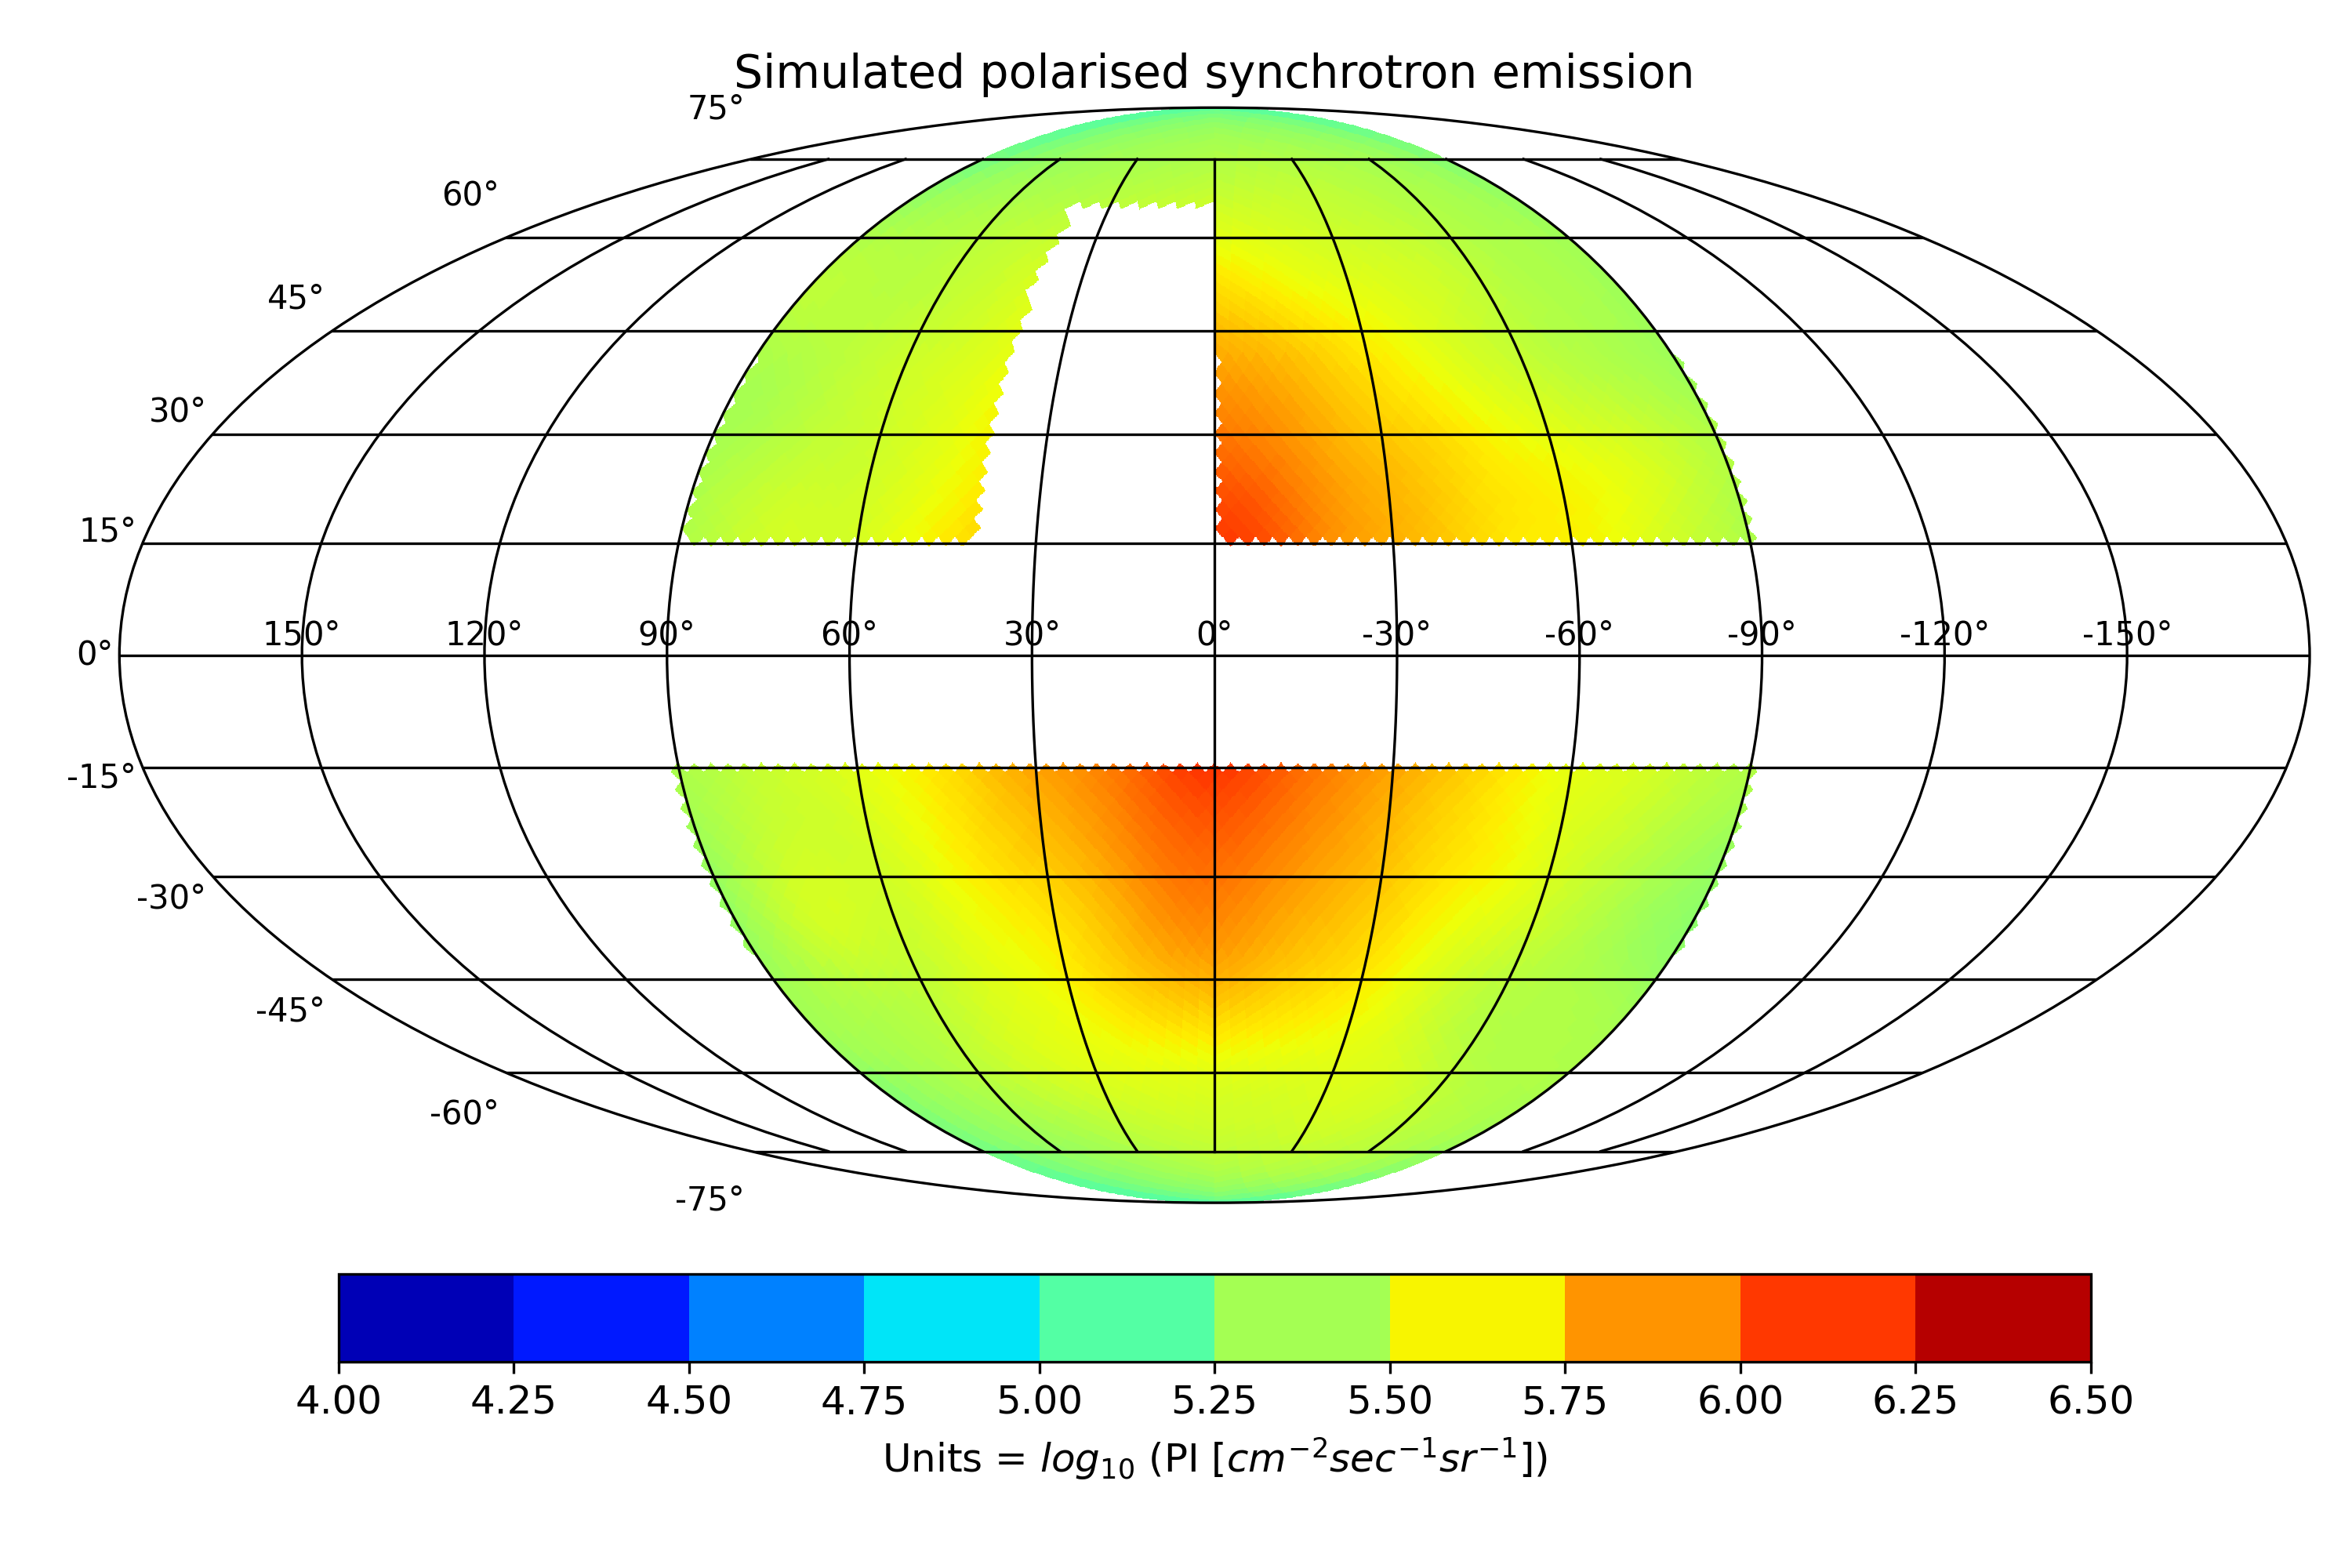
\includegraphics[width=9cm]{Images/Jan-20-2022Ver1_Skymap_Bstr_3_Btur_6_Rmag_5_Zmag_7_norm_3.76e-13.png}
        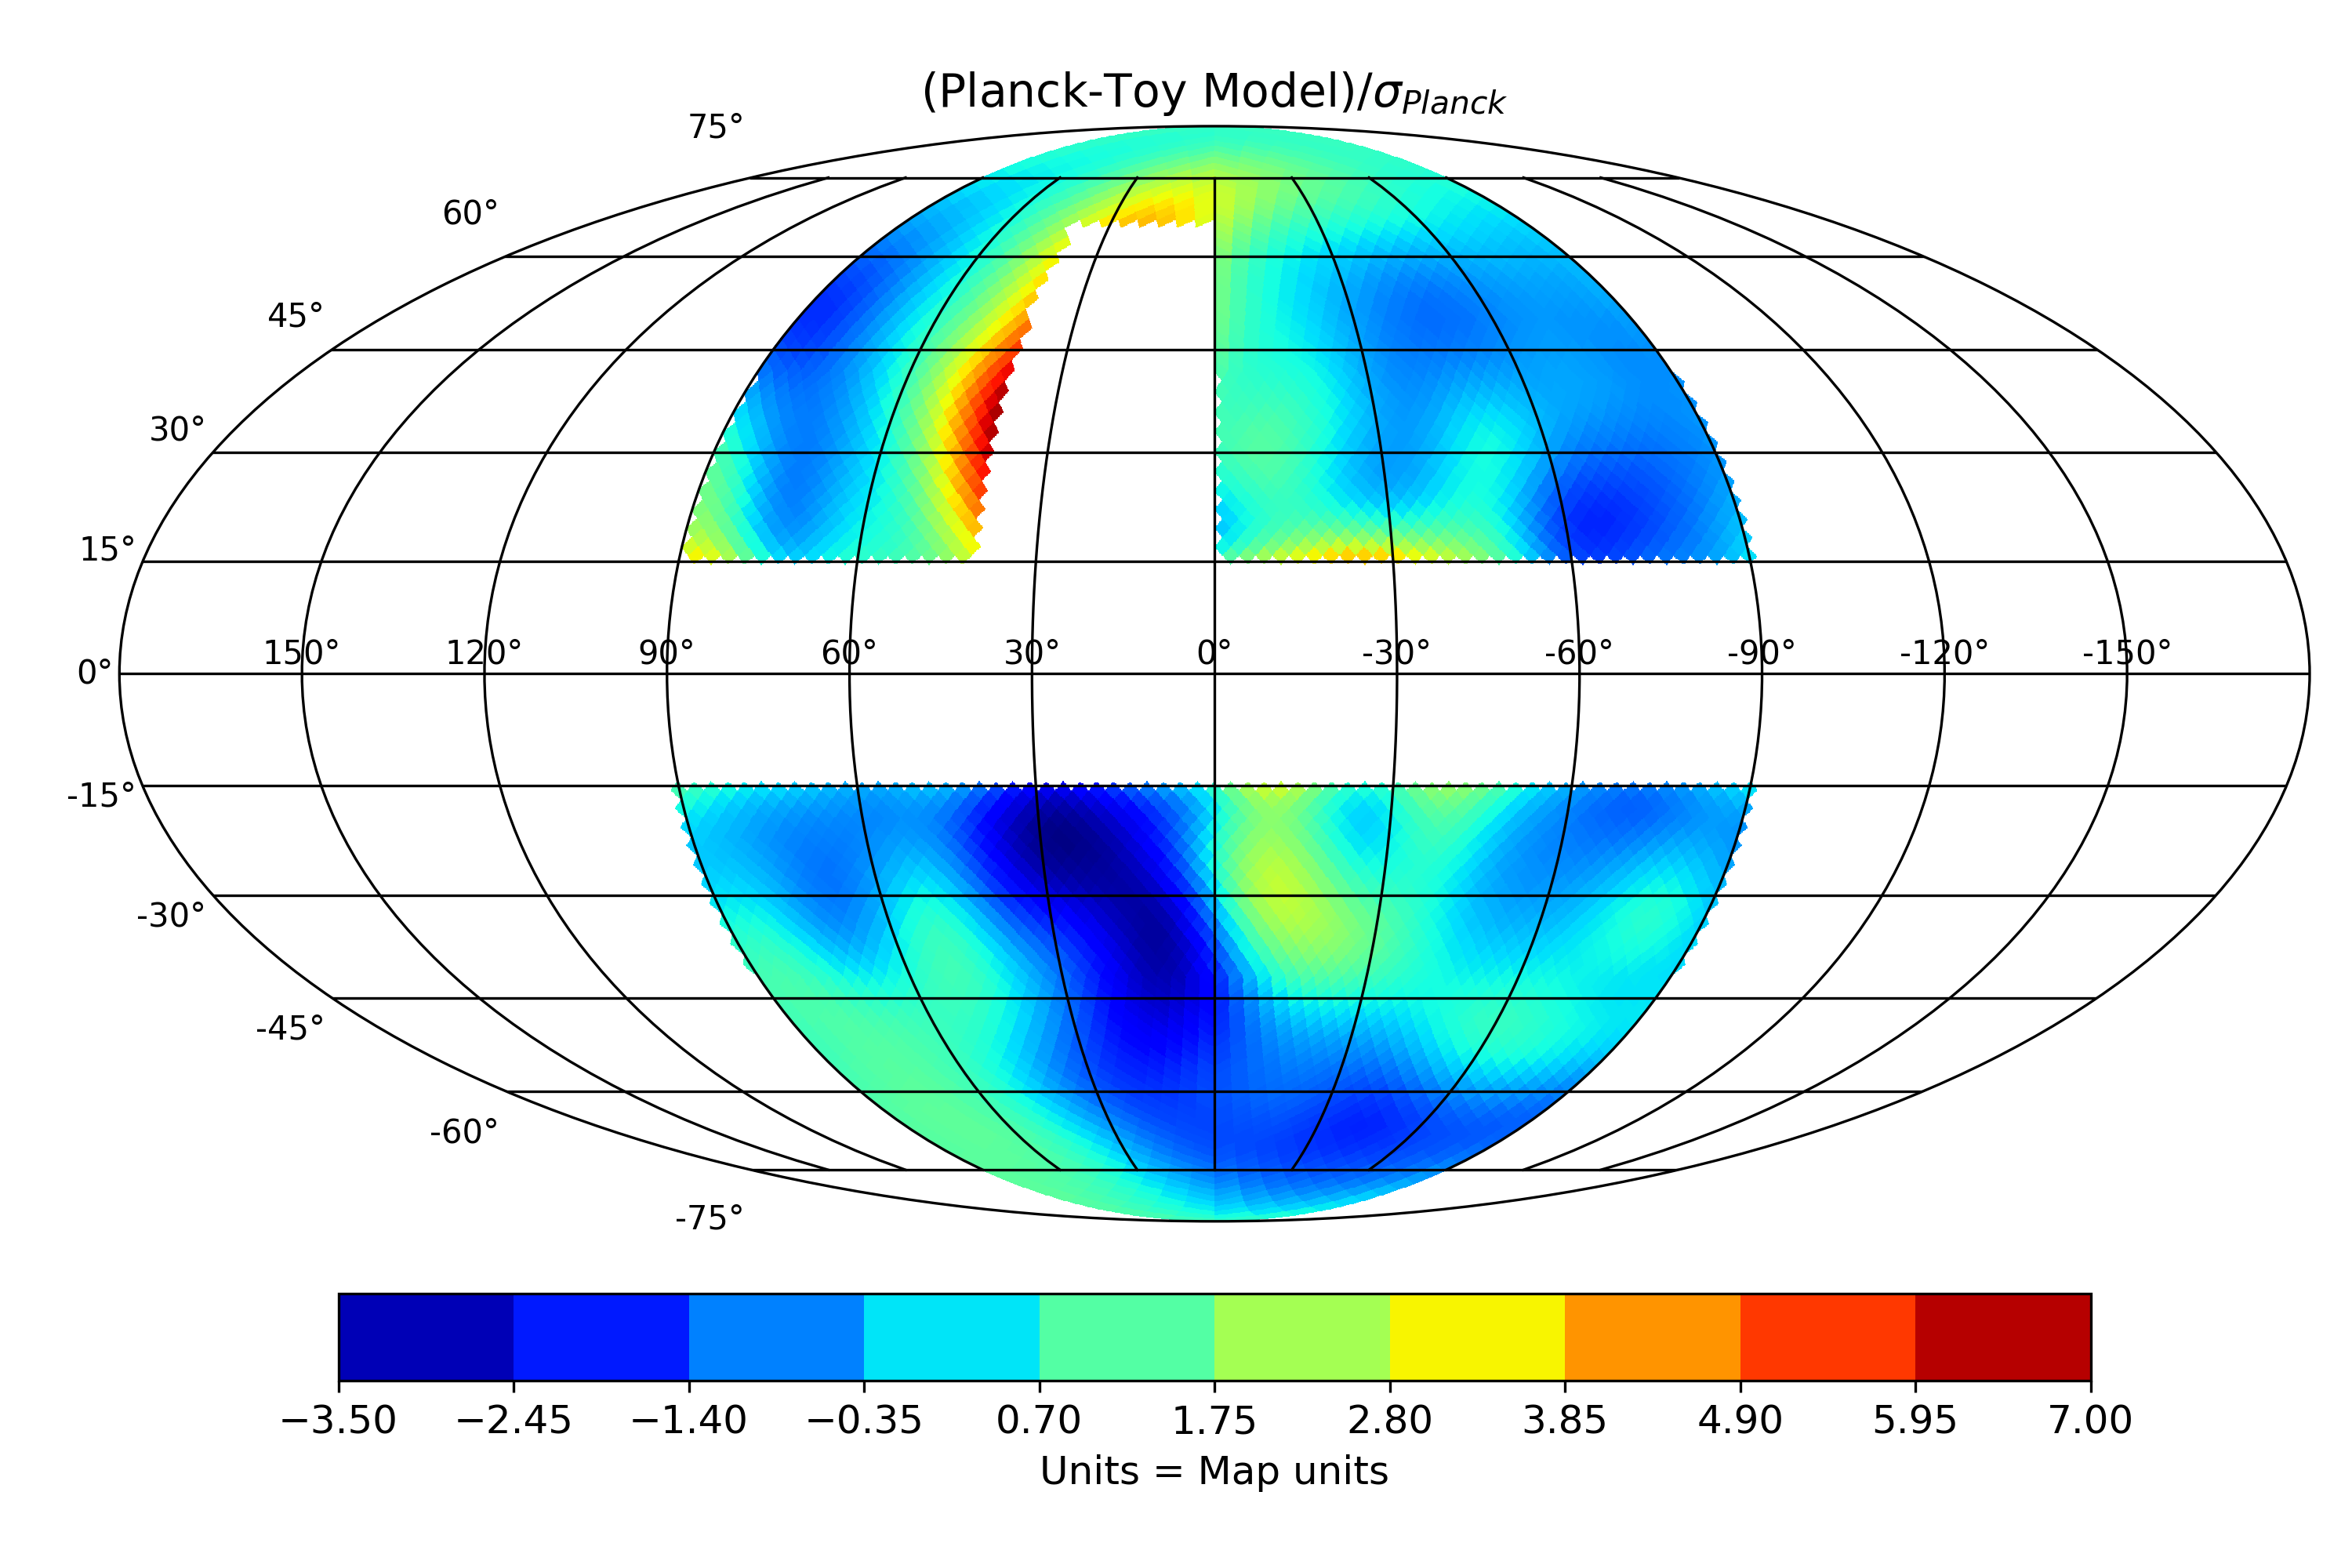
\includegraphics[width = 9cm]{Images/Jan-20-2022_Residue_Bstr_3_Btur_6_Rmag_5_Zmag_7_norm_3.76e-13.png}%
        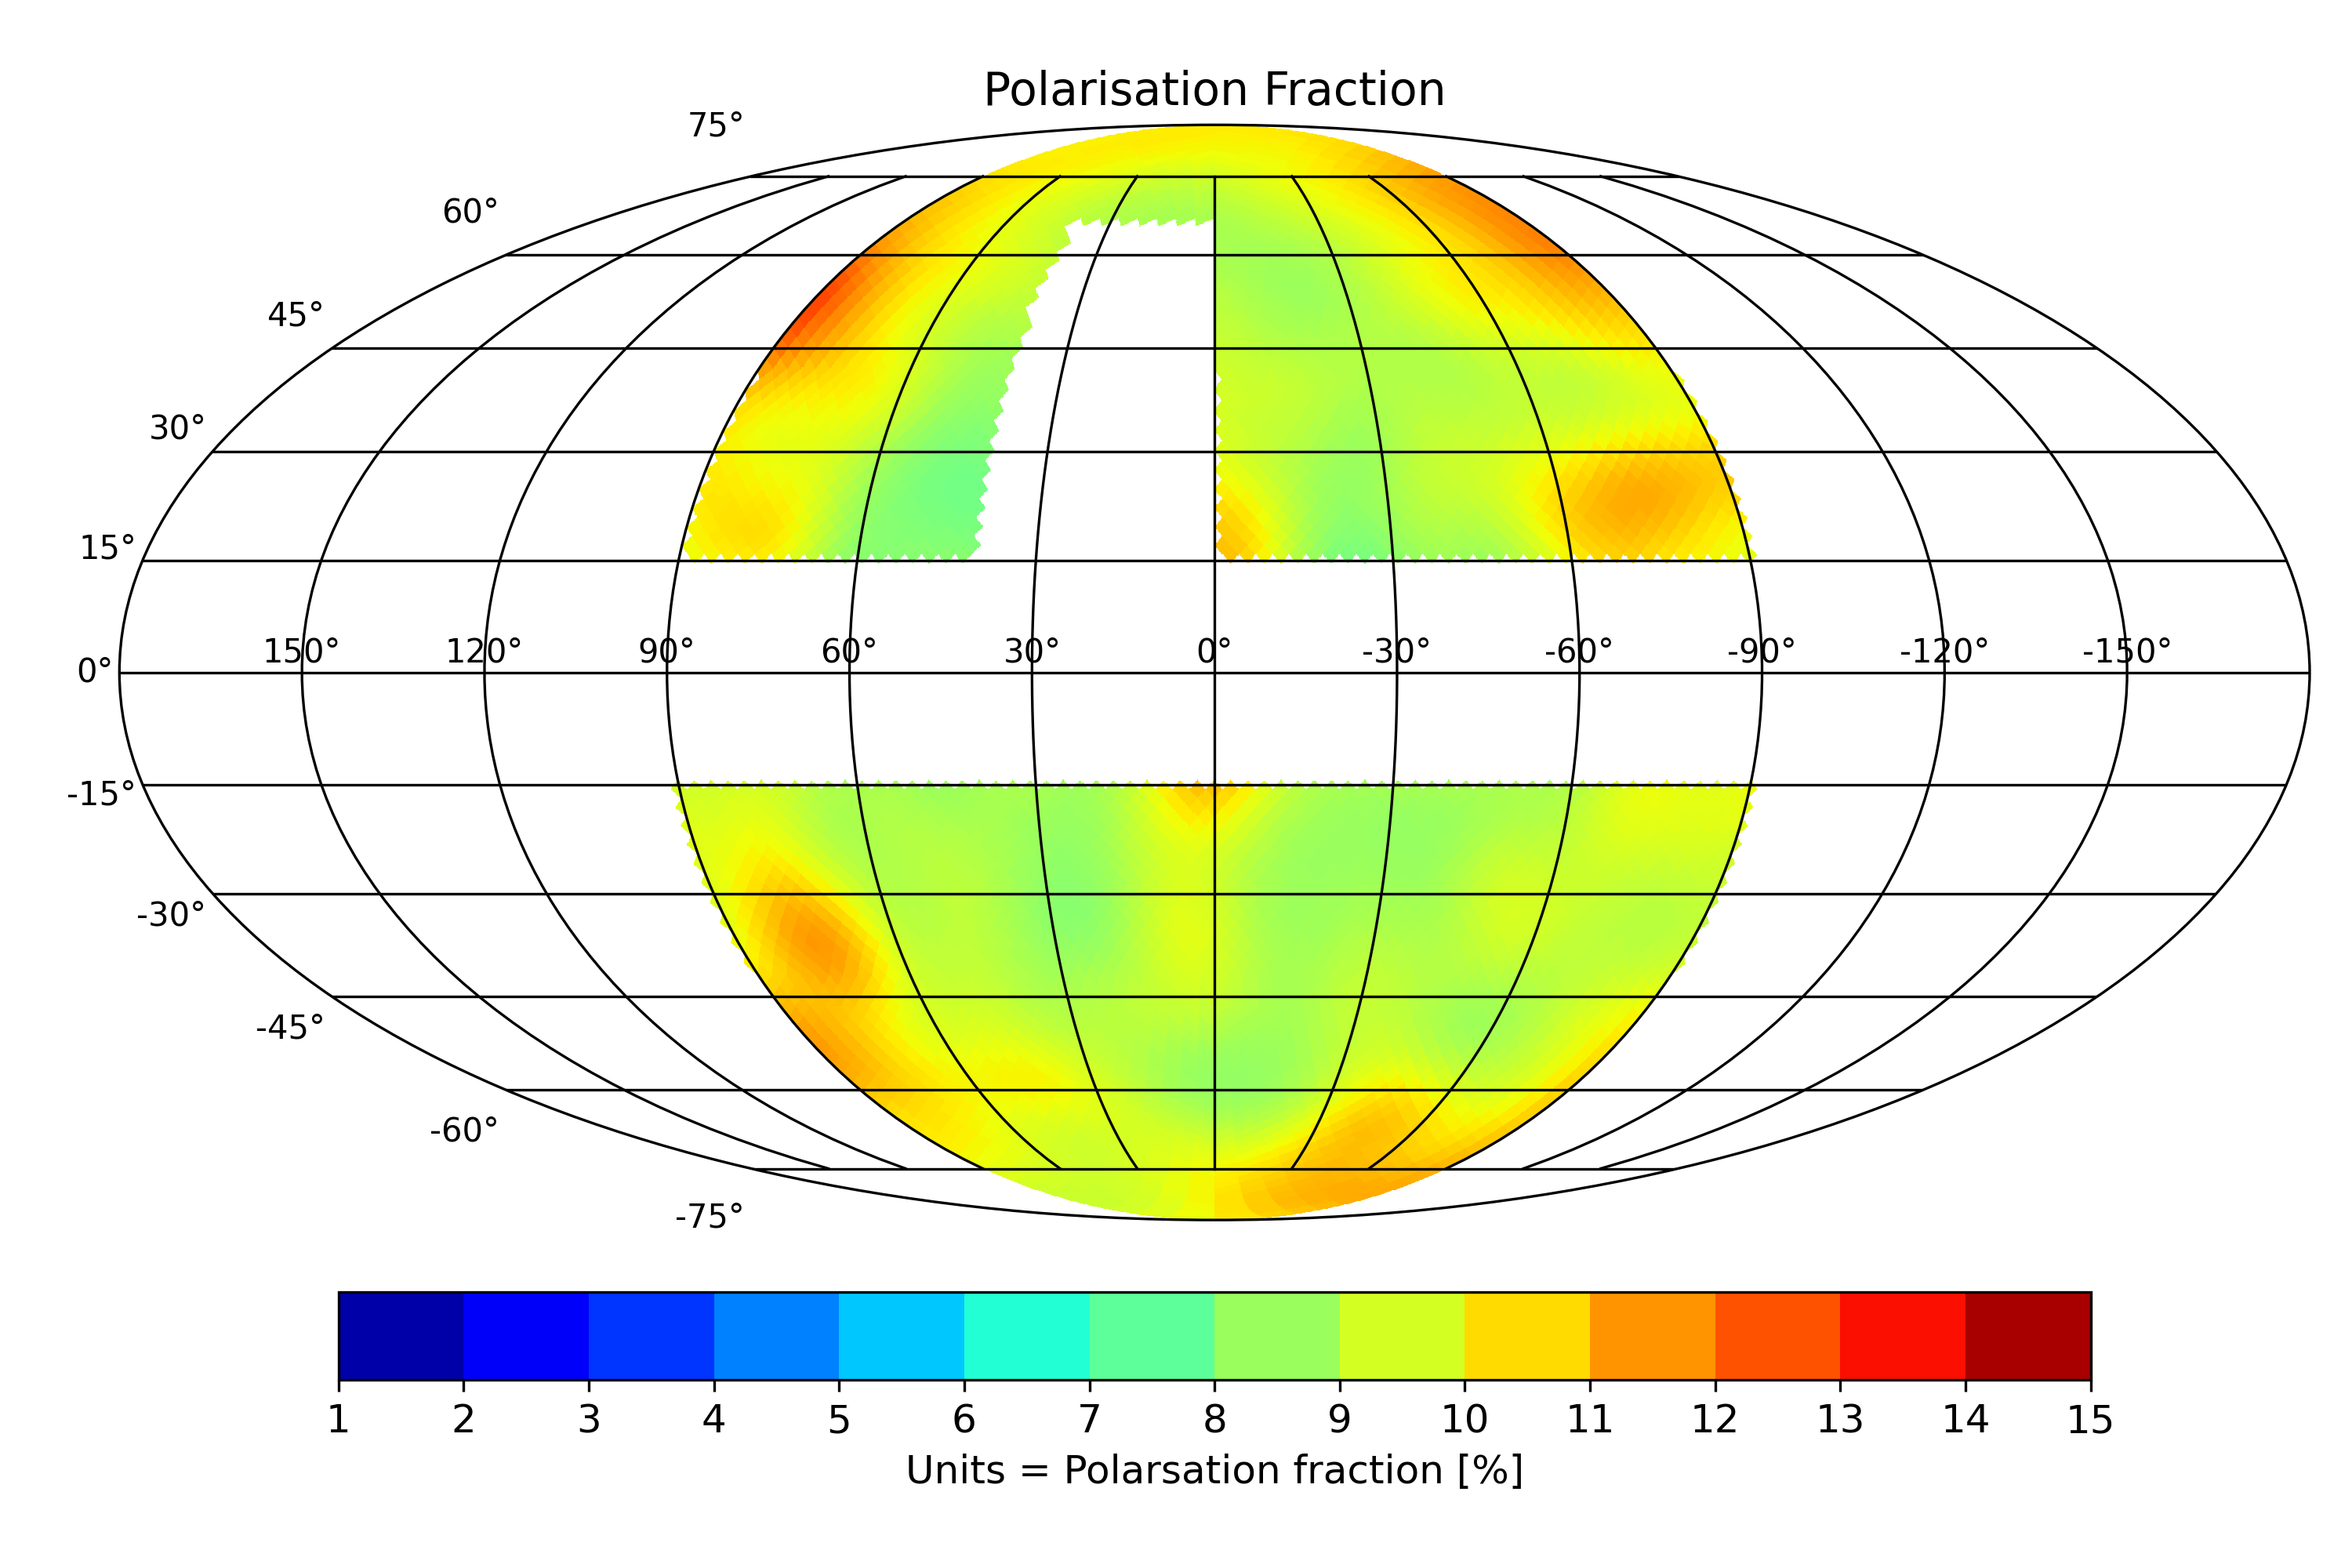
\includegraphics[width =9cm]{Images/Jan-20-2022_Pol_Frac_30GHz_Total_Skymap_Bstr_3_Btur_6_Rmag_5_Zmag_7_norm_-1.24e+01.png}

    \caption{\textbf{Top:} Planck polarised emission (\textbf{left}) and simulated polarised emission skymap from best fit parameters (see table ~\ref{Para_table})
            \newline \textbf{Bottom:} Residual of observation and simulated data (\textbf{left}) and polarisation fraction for toy model (\textbf{right}).}
    \label{fig:Skymaps}
\end{figure}

\newpage
%% Uncertainities in the parameters
\label{Para_table}
\begin{center}
\begin{tabular}{ |p{4.cm}|p{4.5cm}|p{6.5cm}|  }
\hline
\multicolumn{3}{|c|}{Best-fit value with 1-$\sigma$ constraint} \\
\hline
Parameter & Best-fit value &Description \\
\hline
\hline
$B_{\mathrm{str}} $& $3_{-1}^{+8} ~ \mu$G & Structured field strength \\
\hline
$B_{\mathrm{tur}} $& $ 6_{-2}^{+12} ~\mu$G & Turbulent field strength\\
\hline
$R_{\mathrm{Mag}}$ = $R_{\mathrm{el}}$ & $5_{-1}^{\infty}$~kpc & Radial cut off \\
\hline
$Z_{\mathrm{Mag}}$ = $Z_{\mathrm{el}}$ & $7_{-1}^{+1}$~kpc & Azimuthal cut\\
\hline
${\rm{log_{10}}}(C_{\rm norm} [{\rm cm}^{-3}]$) & ${-12.43}_{{-1.31}}^{{+0.32}}$ & Electron normalisation at 10~GeV\\
\hline
\end{tabular}

\end{center}


\section{Cosmic ray deflections from different magnetic field models}
\label{Deflections}

It is known that when a charged particle is moving in a magnetic field, it gyrates along the field lines by virtue of the Lorentz force. The radius of the circular motion that the particle undergoes is called the Larmor radius $r_L = \frac{\beta \gamma m\rm{c^2}}{Z\rm {e}B}$, $\gamma m\rm{c^2}$ is the energy ($E$) of the cosmic ray, $Z$ is the atomic number and $\beta = 1$ for cosmic rays. 
UHECRs also undergo the same Lorentz force when propagating through Galactic magnetic fields. The extra-Galactic magnetic field is rather weak $B = \rm few ~ nG$ and the ultra-high energy cosmic rays UHECRs $E > 10^{18}$ EeV are not sensitive to them. However, once they enter the Galaxy magnetic fields are of the order of few $\mu$G. In case for a proton at 6~EeV in $6~\mu$G field the $r_L \approx 1 ~ \rm kpc$ , this implies that the proton will be subject to deflection by the large scale Galactic magnetic fields.


The propagation of the UHECRs is one of the one of the less understood phenomena in high energy physics. The propagation of cosmic rays is vital to understand their sources and this is in turn is sensitive to their deflection by magnetic fields.In this section we address the deflections of UHECRs using a toy model. The aim of this study is not to depict reality but to understand how simple structured and turbulent halo magnetic field model interacts with extra-Galactic cosmic rays. 

To propagate the cosmic rays we used the CRPropa3's \cite{CRPropa3_2016} Boris pusher which is a type of solver for Lorentz equations. CRPropa conserves the total energy and momentum of each particle during the propagation.  \Vasu{Arjen may be you have some comment on this ?!}
To achieve this we backtrack $10^7$ cosmic rays starting isotropically from earth to a distance of 20~kpc with a trajectory length of 300~kpc. We use nitrogen as a choice of our cosmic ray particles at 40~EeV energy. 


In figure~\ref{fig:AD_Plots} we show two kinds of plots, \textit{1)} the histogram of all sky in log (density/str) of the backtracked positions for the cosmic rays (\textbf{left}), there are 180 bins both for longitudes and latitudes.\textit{2)} is the histogram of binned arrival directions of cosmic rays in a $5^{\circ}$ region from two known sources (\textbf{right}) Centaurus A (lat = $\rm 19.42^{\circ}$, lon = $\rm 309.51^{\circ}$) and NGC 253 (lat = $\rm -87.96^{\circ}$, lon = $\rm 309.51^{\circ}$).  We normalise both the skymaps with first making histograms with no-magnetic fields and then dividing the histogram generated using toy model by the former. This gives us a normalised value of the number of hits obtained as seen on the right in the figure~\ref{fig:AD_Plots}.

It can be seen that the best fit and lower extreme parameters can clearly help in associating the deflected particles with their potential source. However, in the case of upper extreme parameters any connection between the point of origin of cosmic rays and their final positions is inconclusive. Cosmic rays from  sources like NGC253 get completely deflected by the magnetic field and hence we obtain a suppressed flux $\approx 5\%$ . In case of Centaurus A the final positions are spread out on the entire sky making it impossible to associate it with the source.

\begin{figure}[h]
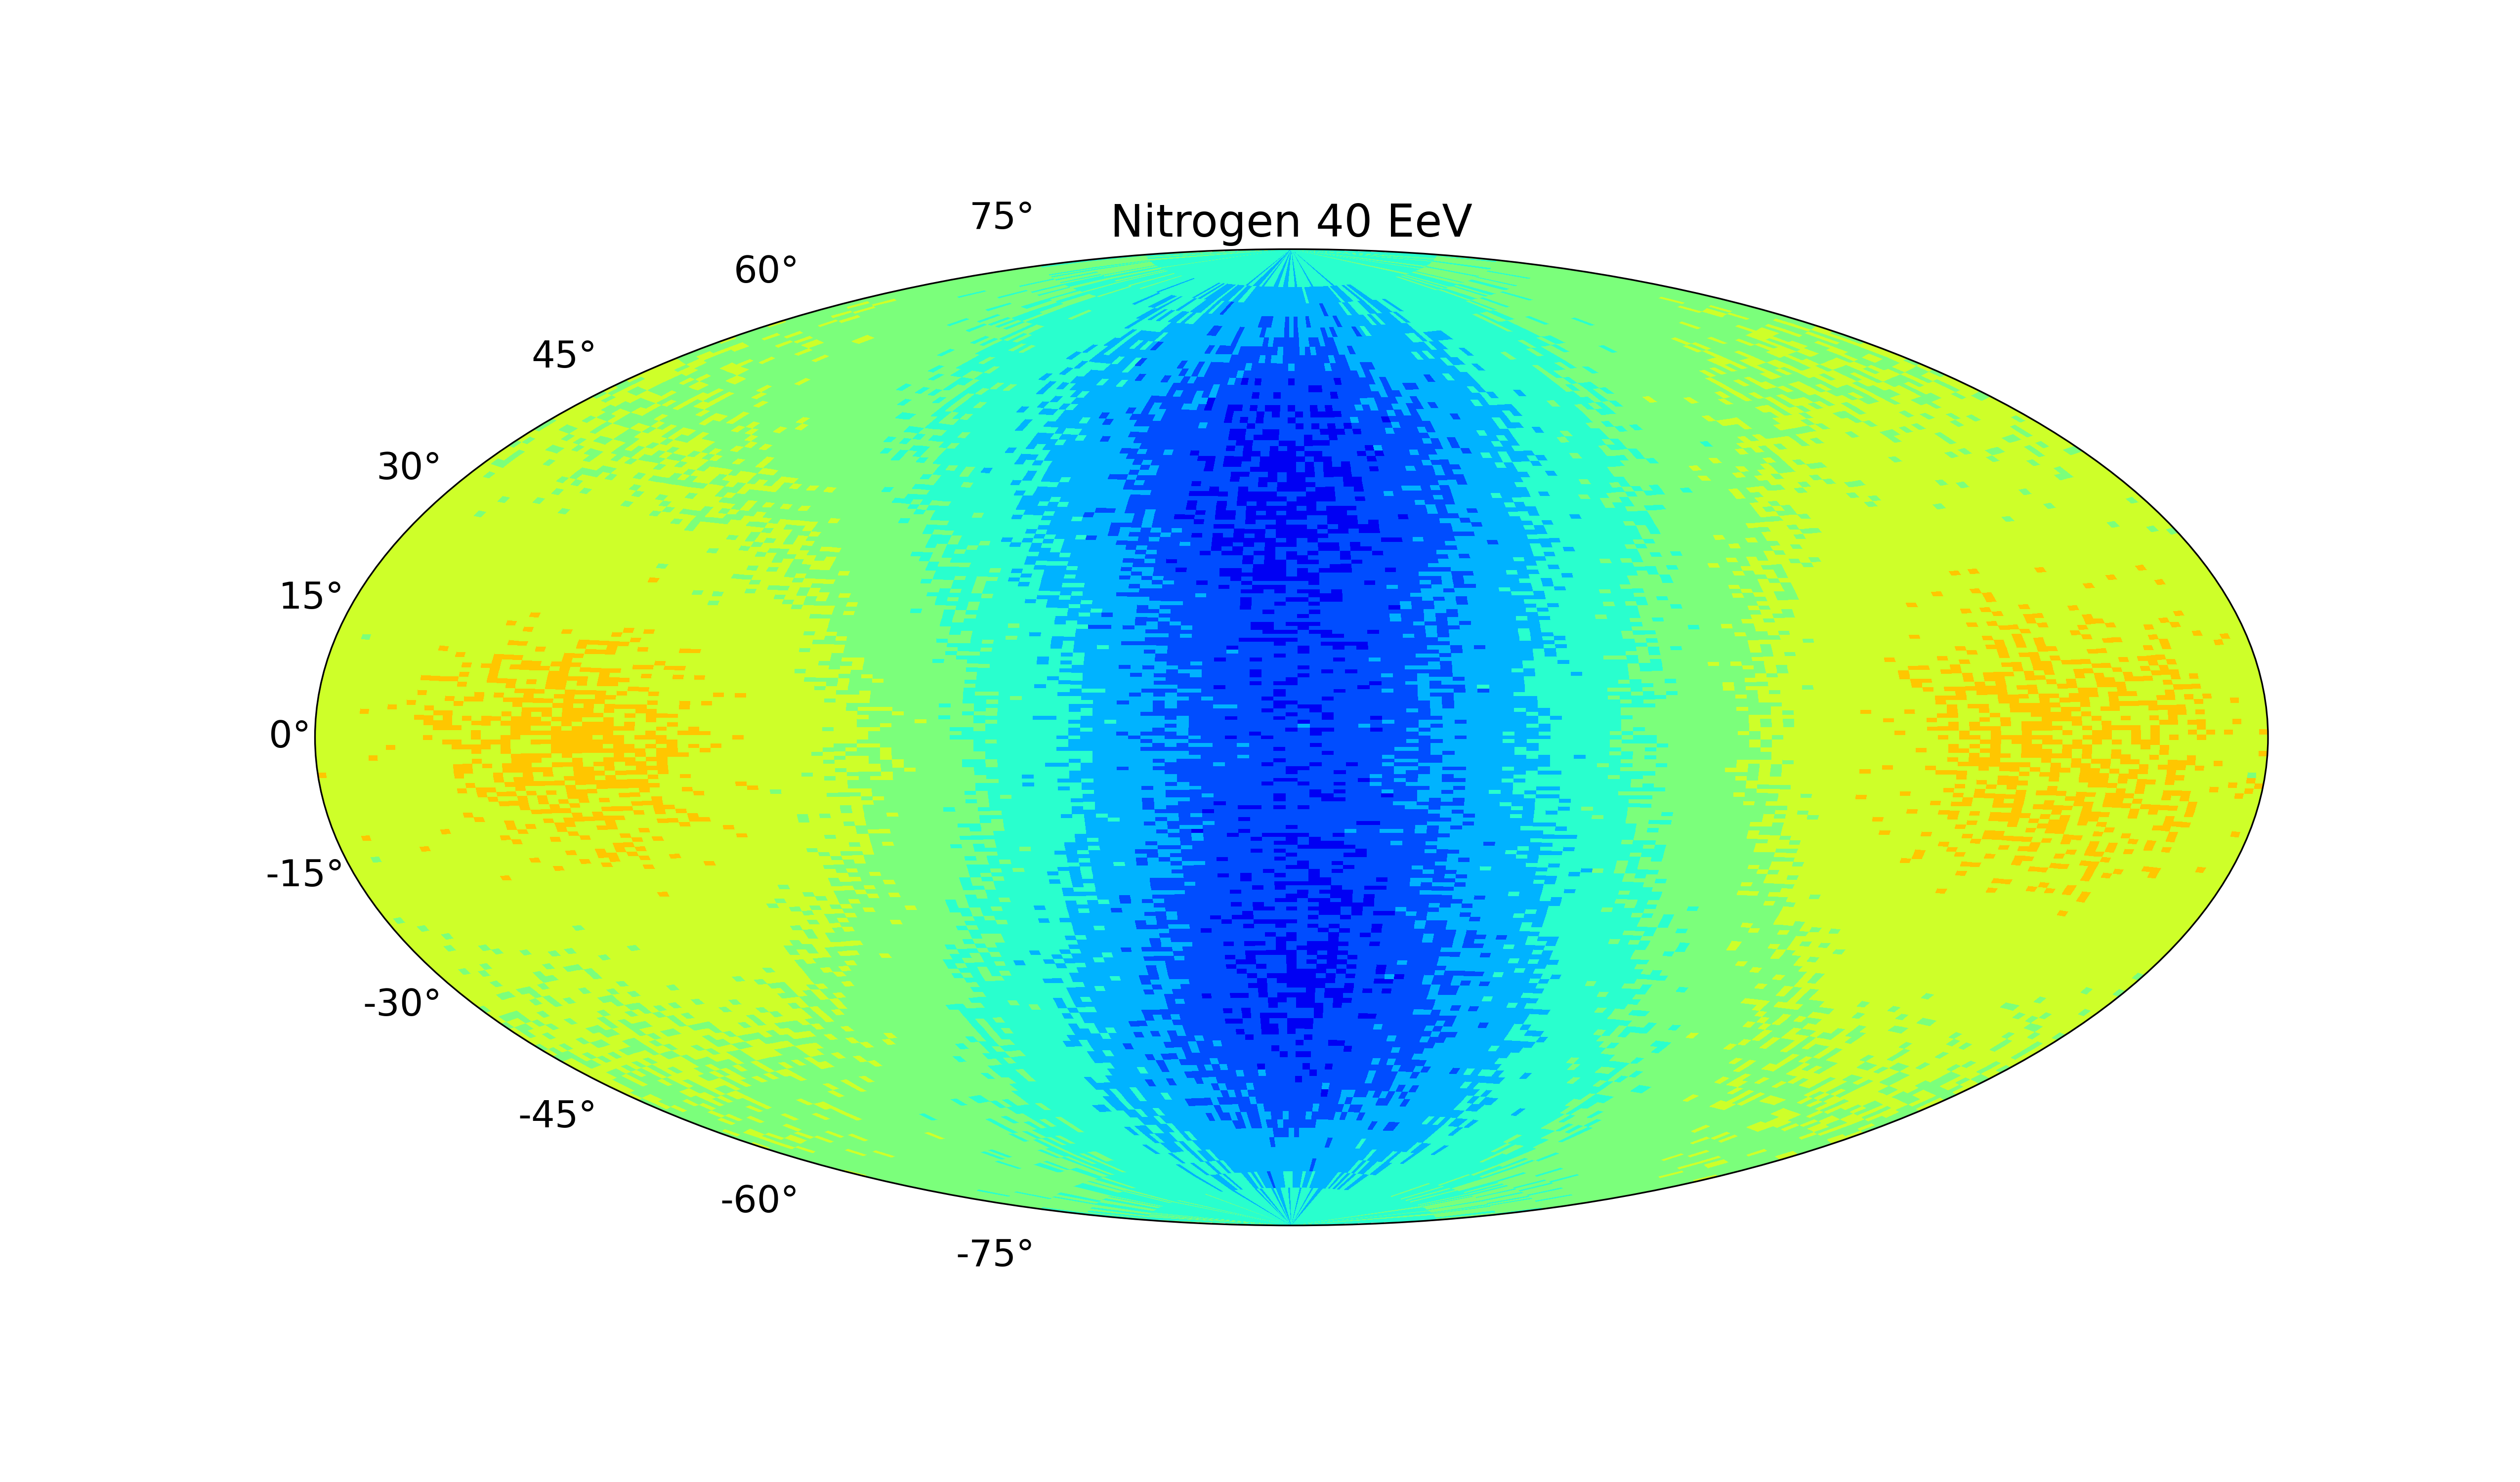
\includegraphics[width=9.0cm]{Images/Log_Bins_180_Historgam_BF_N2_Str_Tur_TM_40_EeV.png}
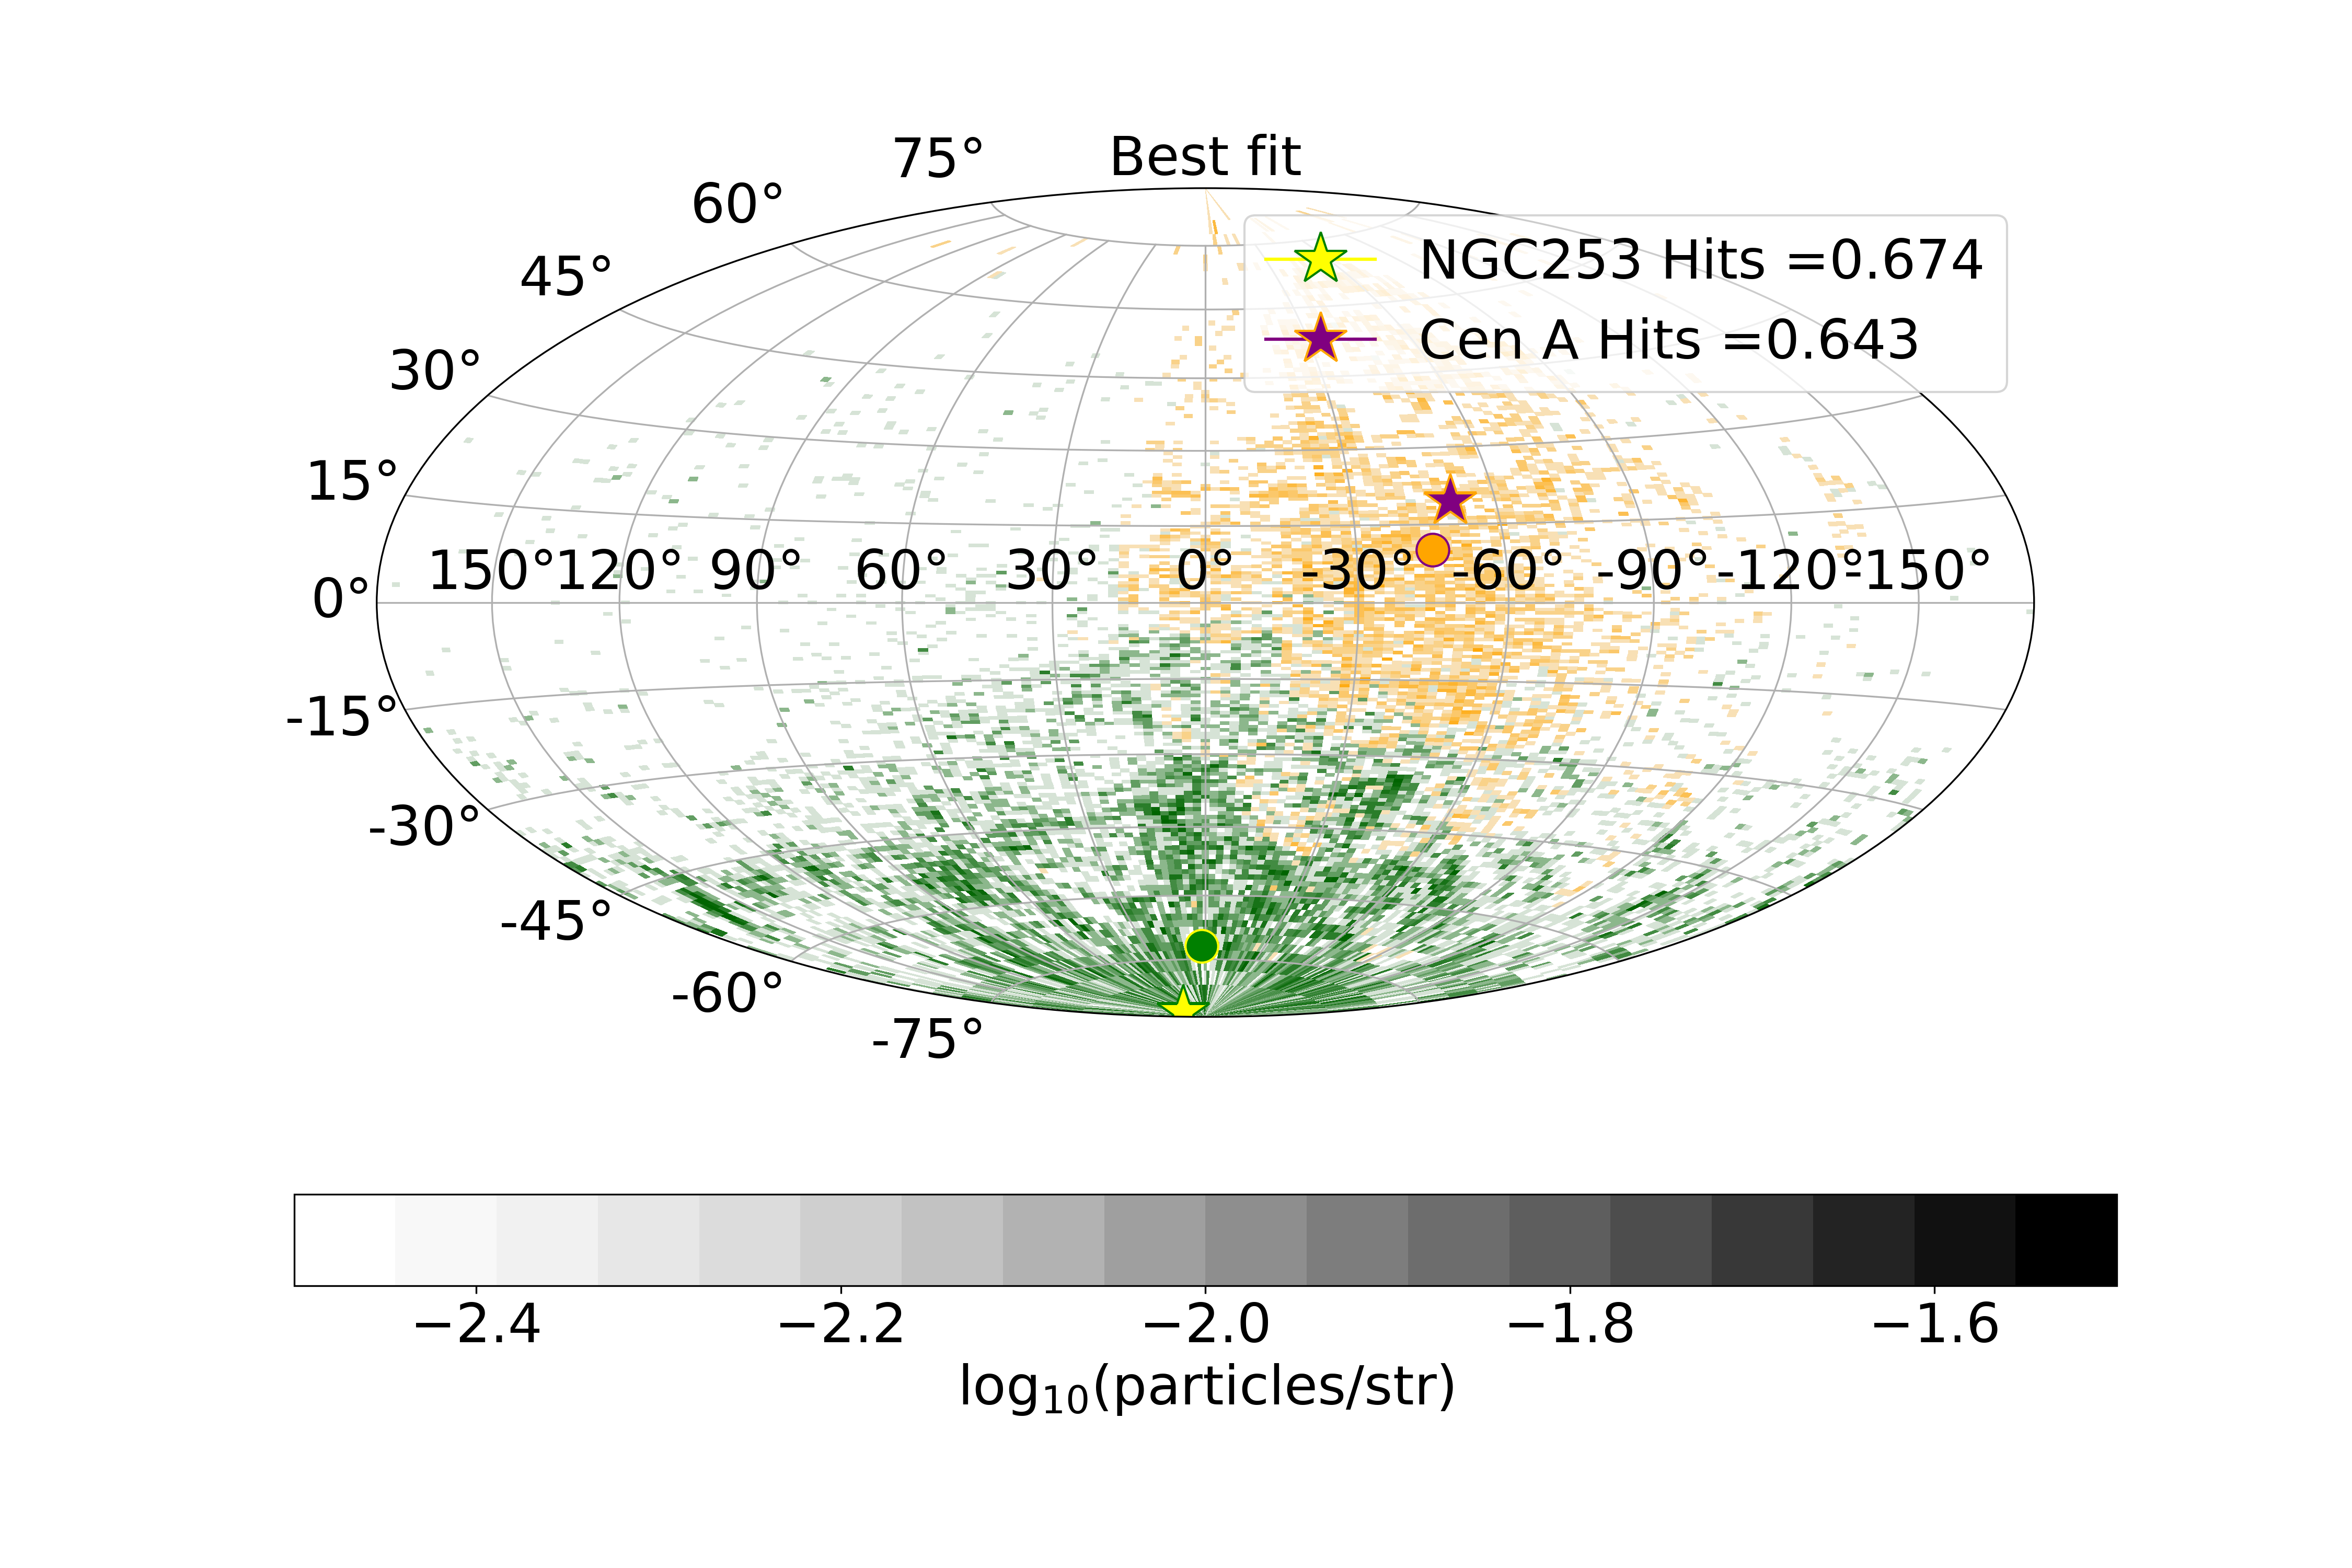
\includegraphics[width=9.0cm]{Images/Bins_180_BF_N2_CenA_NGC253_Str_Tur_TM_40_EeV.png}
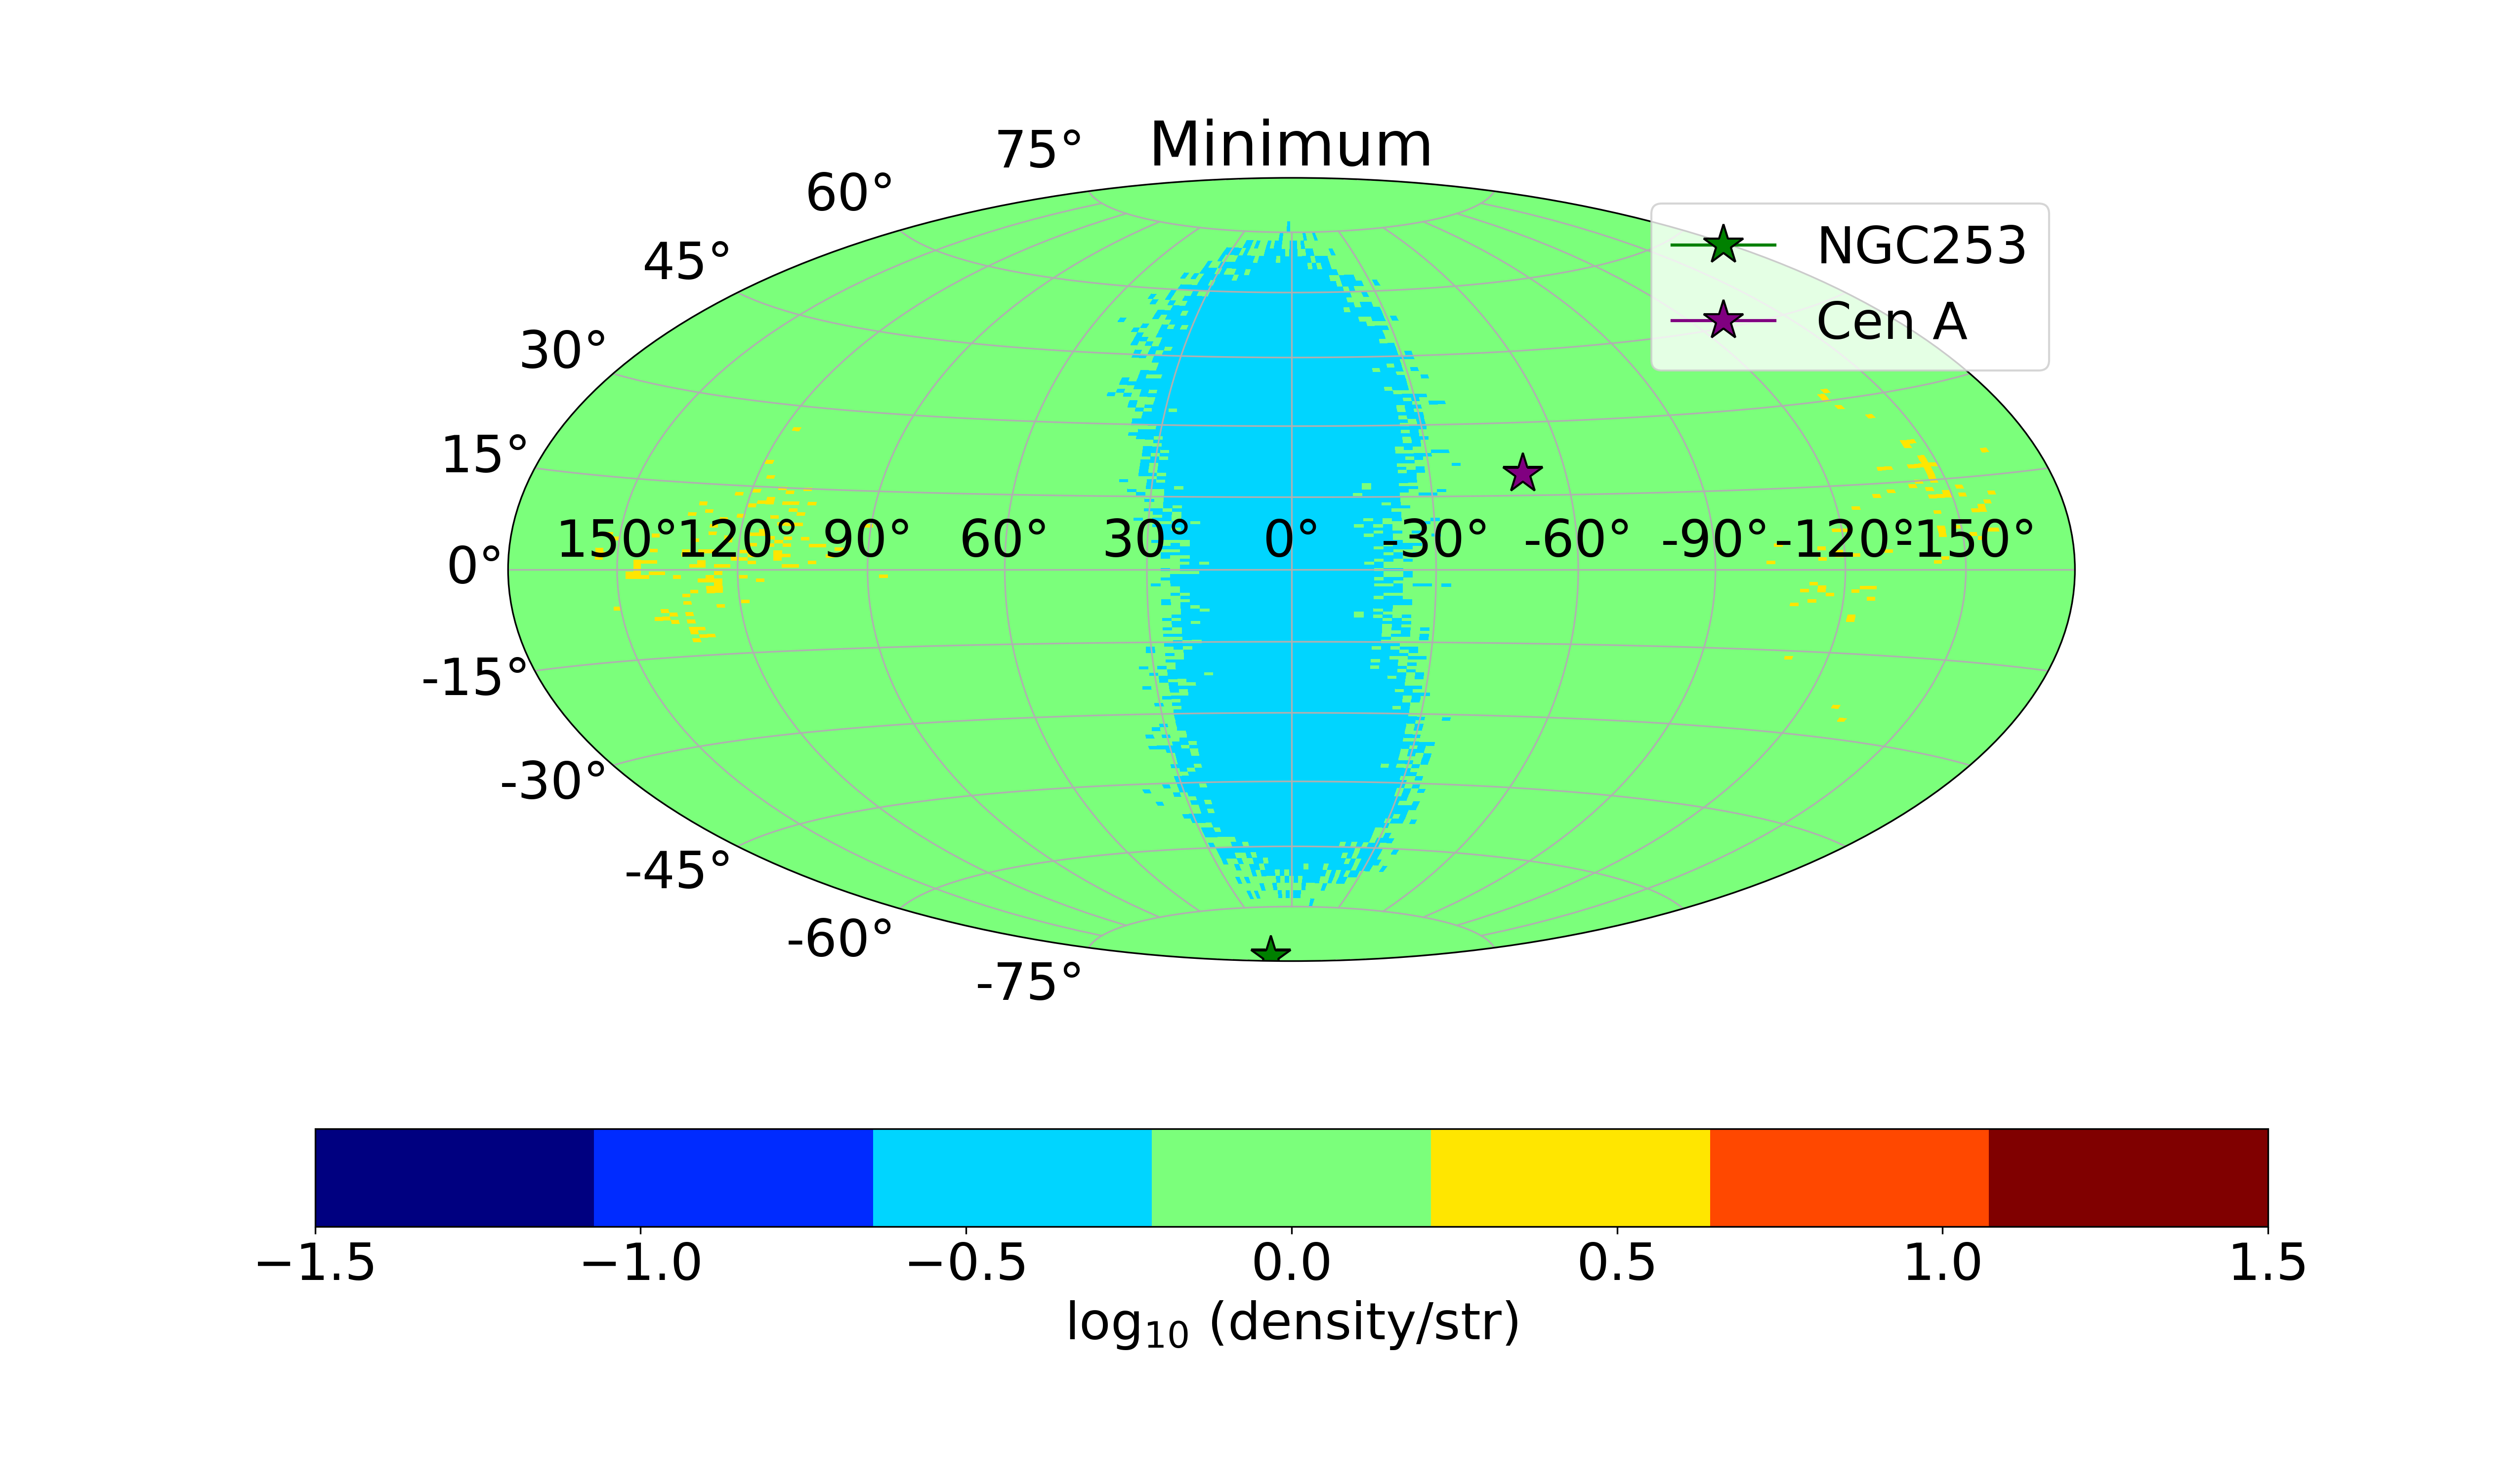
\includegraphics[width=9.0cm]{Images/Log_Bins_180_Historgam_LB_N2_Str_Tur_TM_40_EeV.png}
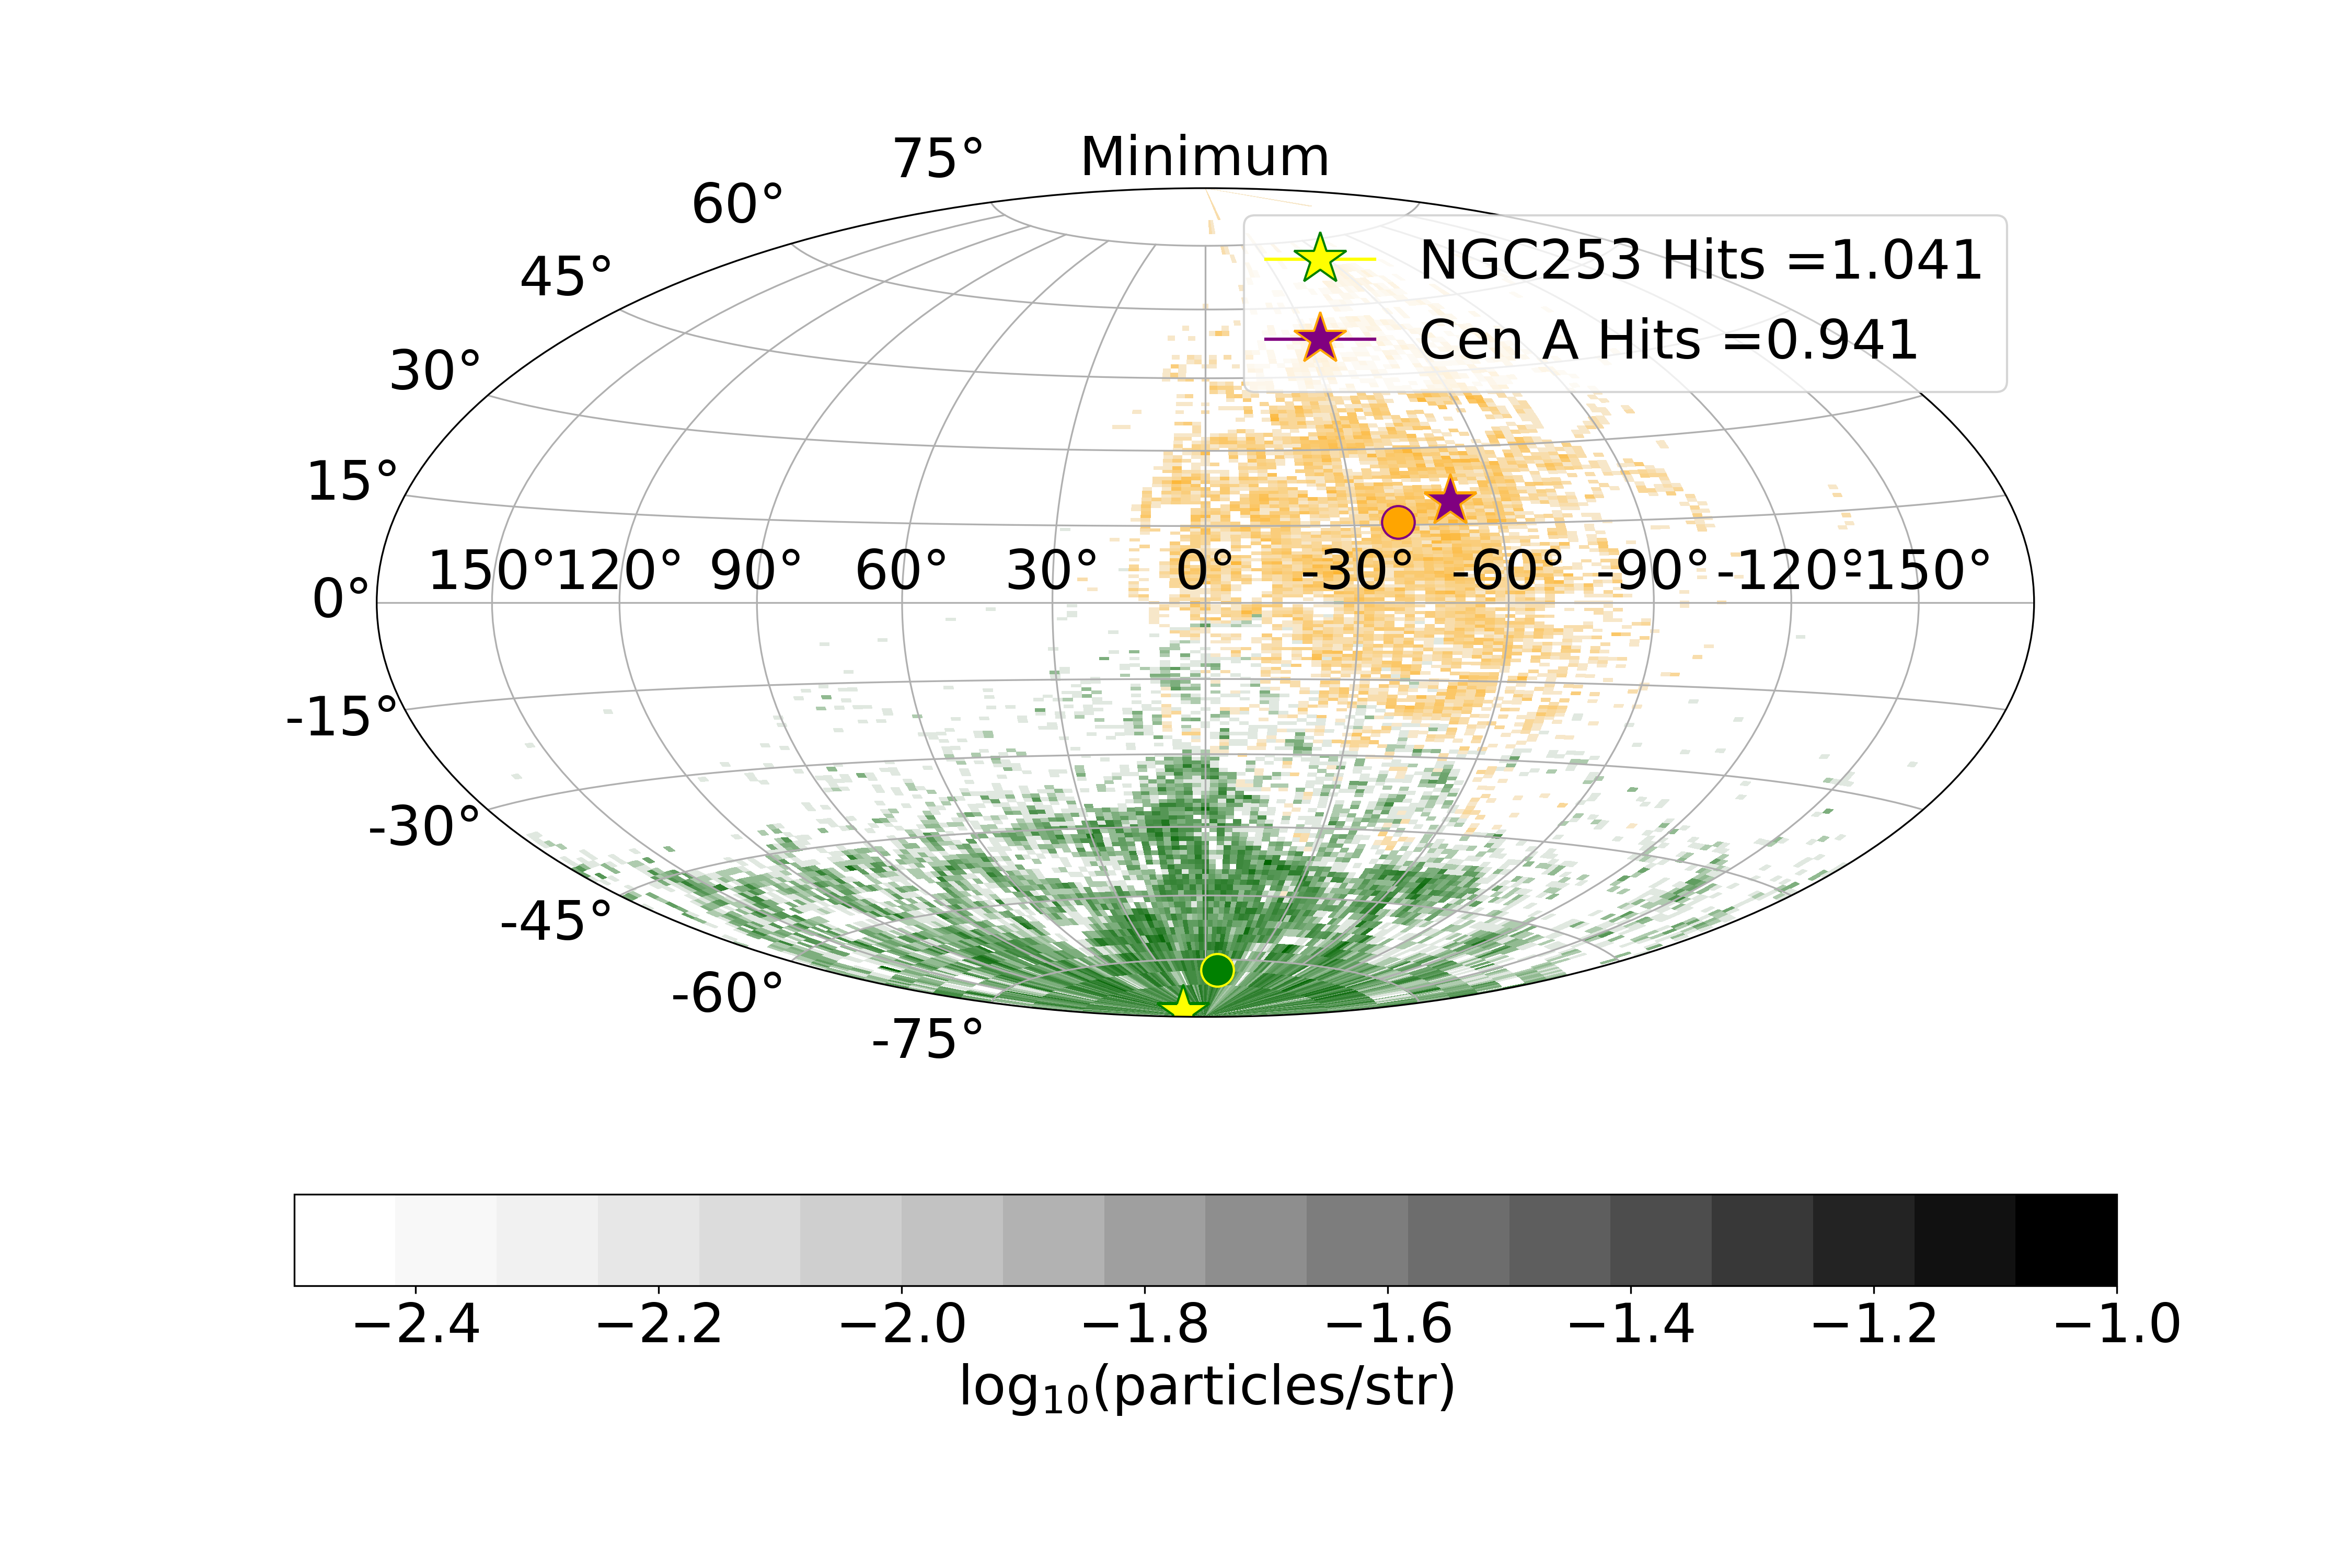
\includegraphics[width=9.0cm]{Images/Bins_180_LB_N2_CenA_NGC253_Str_Tur_TM_40_EeV.png}
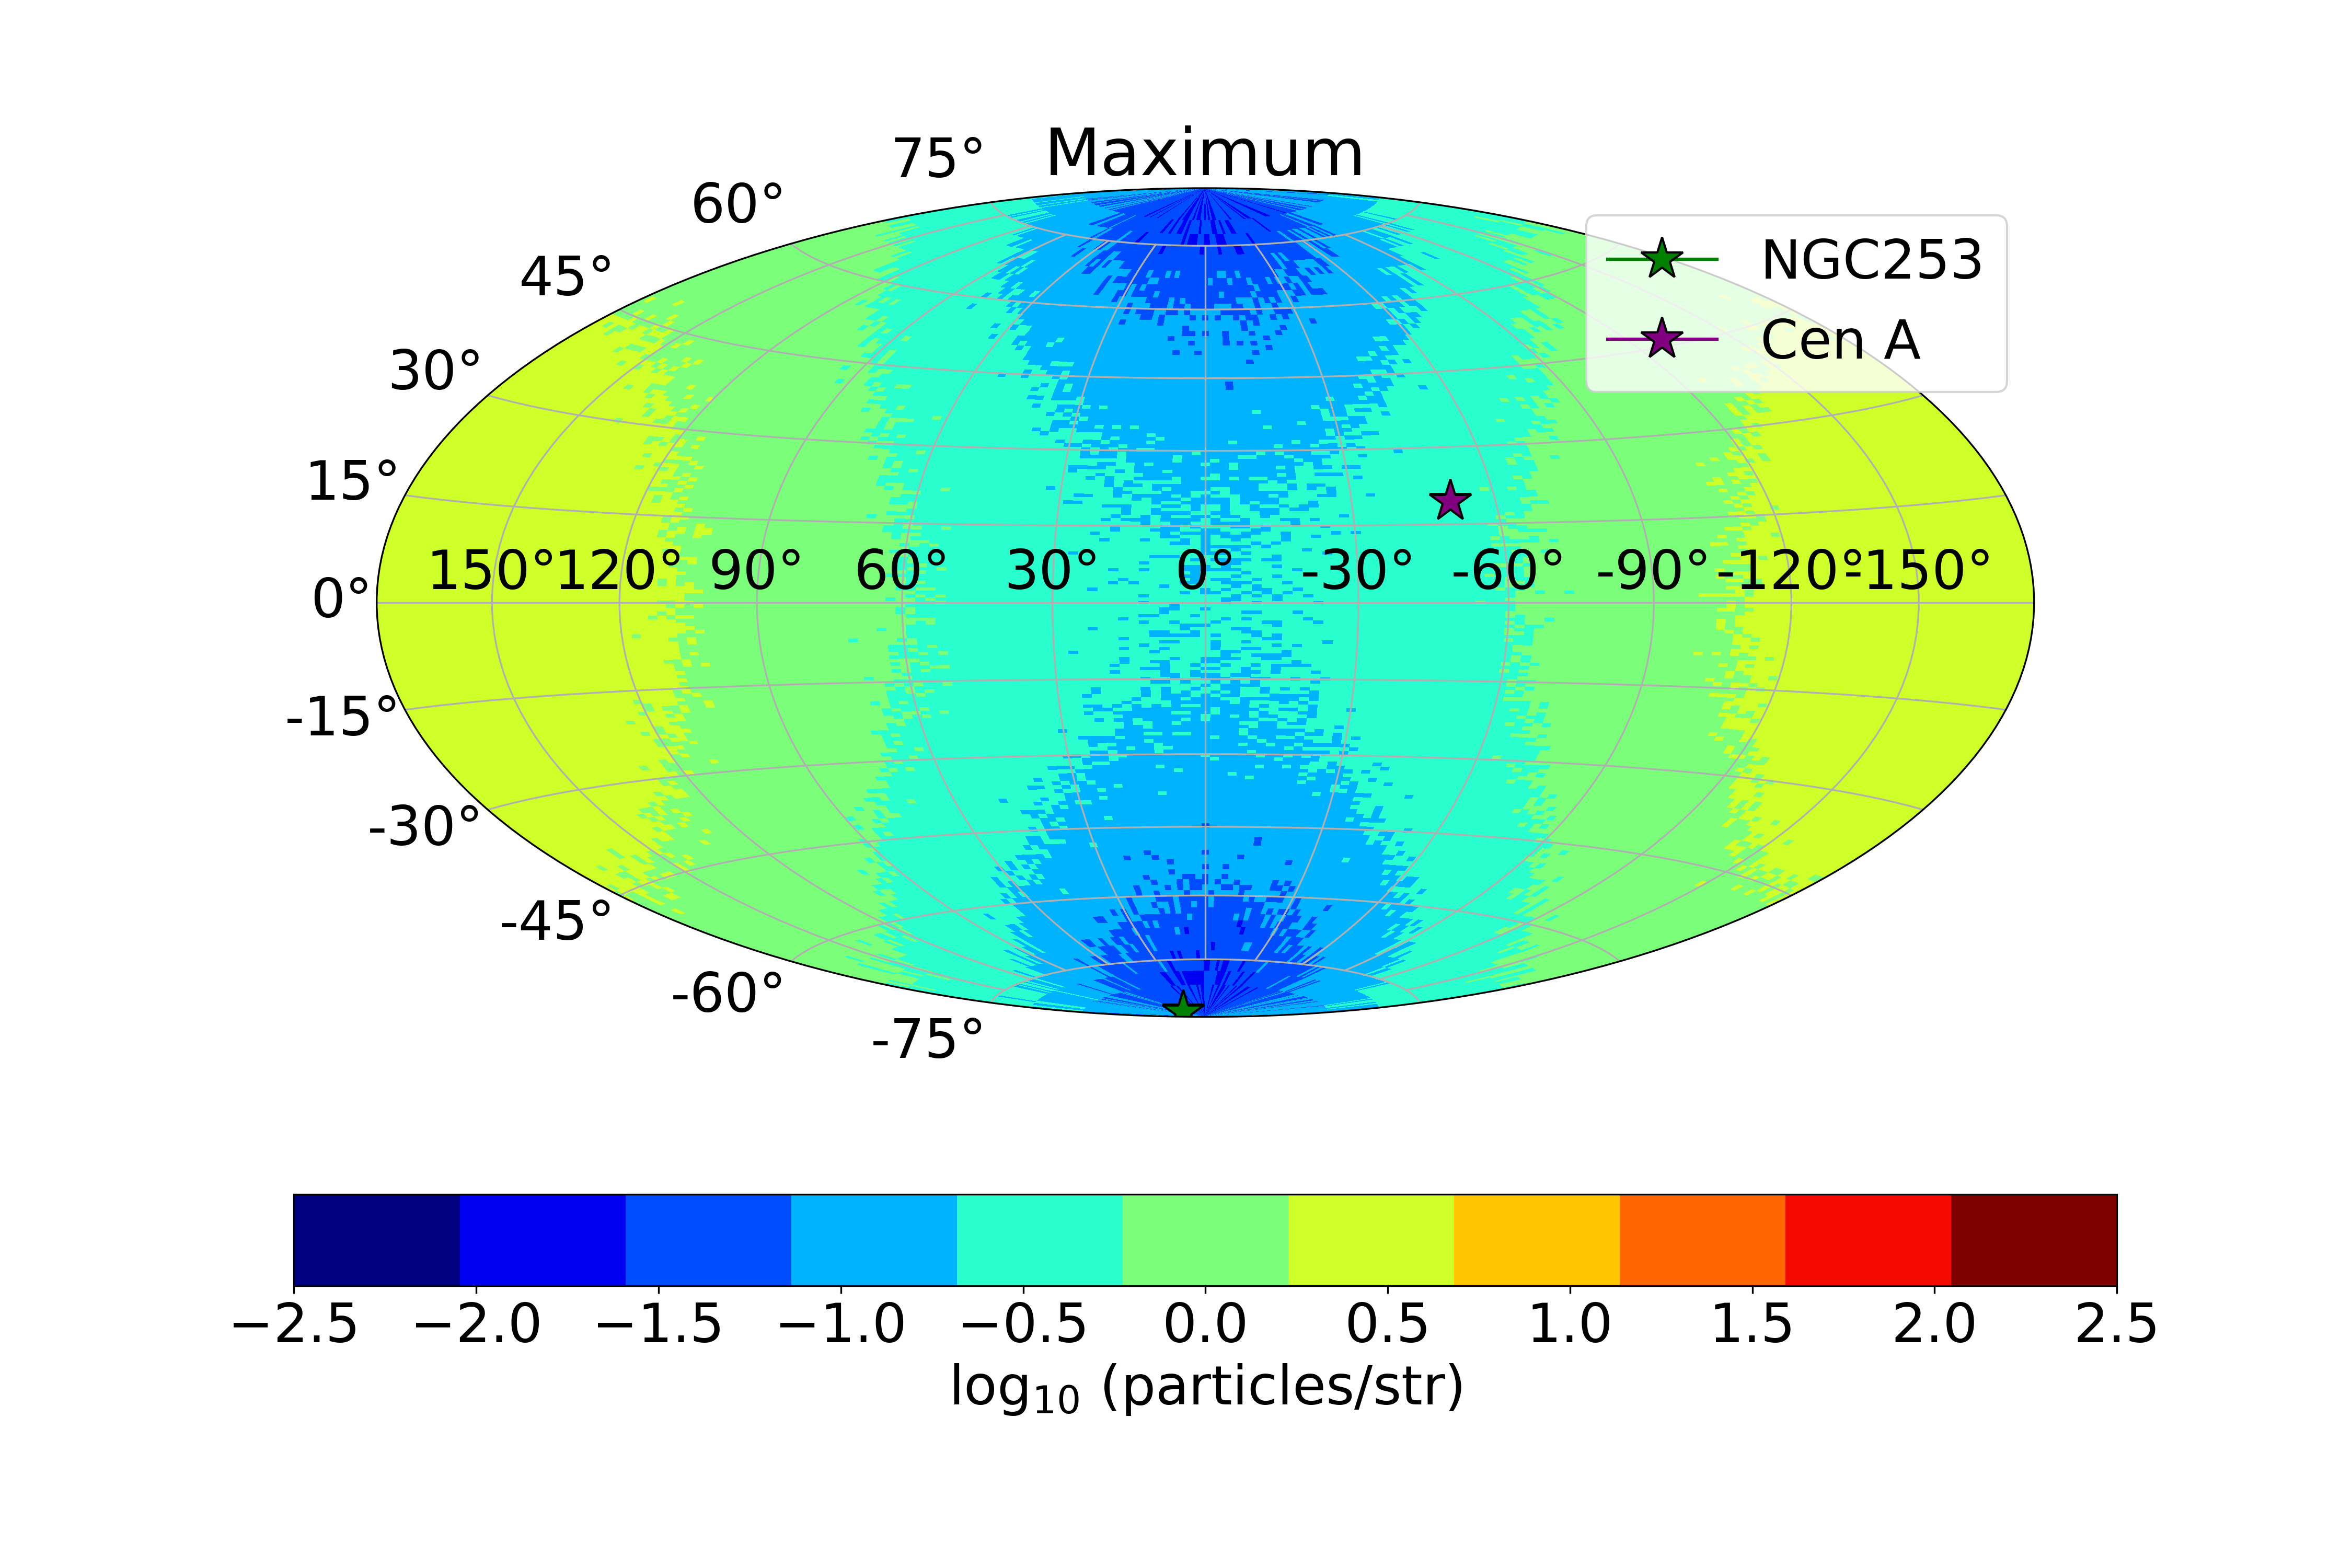
\includegraphics[width=9.0cm]{Images/Log_Bins_180_Historgam_UB_N2_Str_Tur_TM_40_EeV.png}
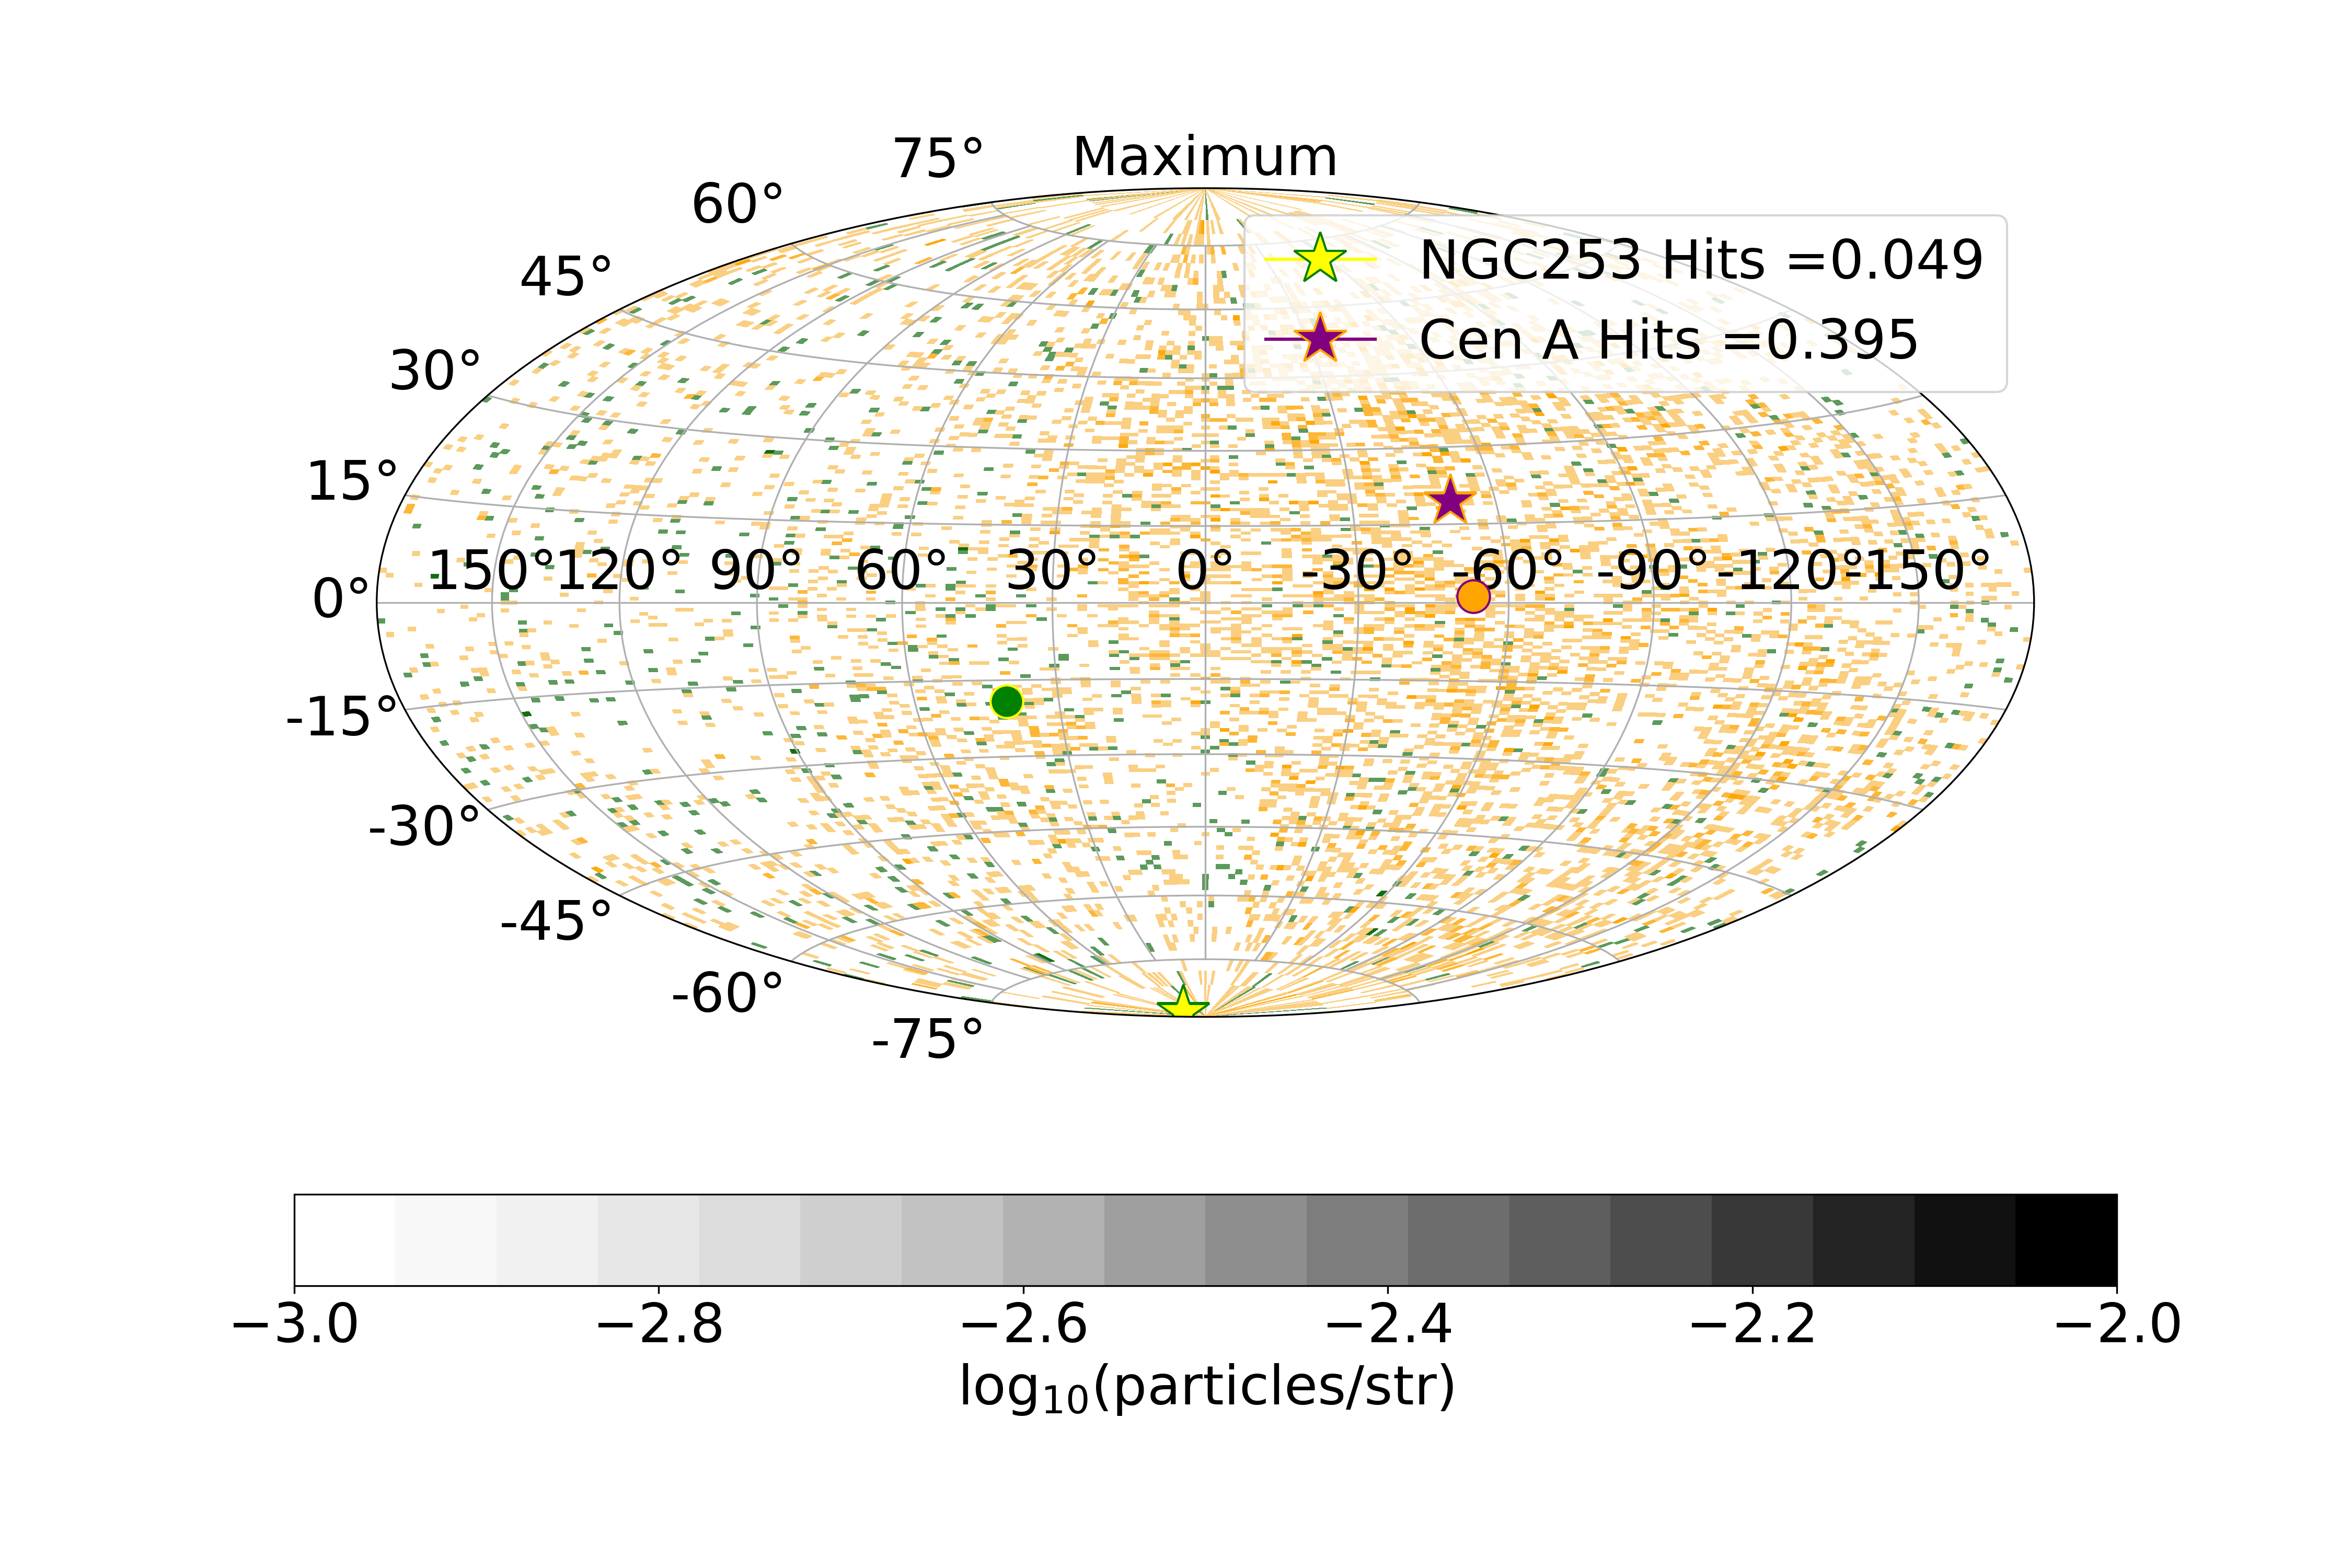
\includegraphics[width=9.0cm]{Images/Bins_180_UB_N2_CenA_NGC253_Str_Tur_TM_40_EeV.png}
\caption{Log brightness of the backtracked positions for cosmic rays shown on \textbf{left} and the arrival directions of the cosmic rays from two known sources Cen A and NGC 253 on \textbf{right} (From table~\ref{Para_table} \textbf{Top} - Best Fit Parameters, {\textbf{Middle} - Lower extreme parameters)} \& {\textbf{Bottom} - Upper extreme parameters, we use $R_{\rm Mag} = $ 20~kpc since that is the maximum extent of the magnetic fields in our simulation.}}
\label{fig:AD_Plots}
\end{figure}
\newpage
\section{Conclusions}
\label{Conclusions}

\clearpage
\section{References}

\printbibliography[heading=none]

\nocite{*}

In table ~\ref{Para_table} we provide the list of all free parameters and the constraints obtained on them.
\newline
%We obtained $1\sigma$ constraint for $B_{\mathrm Mag}$ = [2,9]$\mu$ G,$B_{\mathrm tur}$ = [4,15)$\mu$ G , $R_{\mathrm Mag}$ = [4,5), $Z_{\mathrm Mag}$ = [6,7) and $C_{\mathrm norm}$= $\mathrm{(5\times 10^{-14},8.83}\times 10^{-13}]$. 

\begin{figure}[h!]
        \centering
        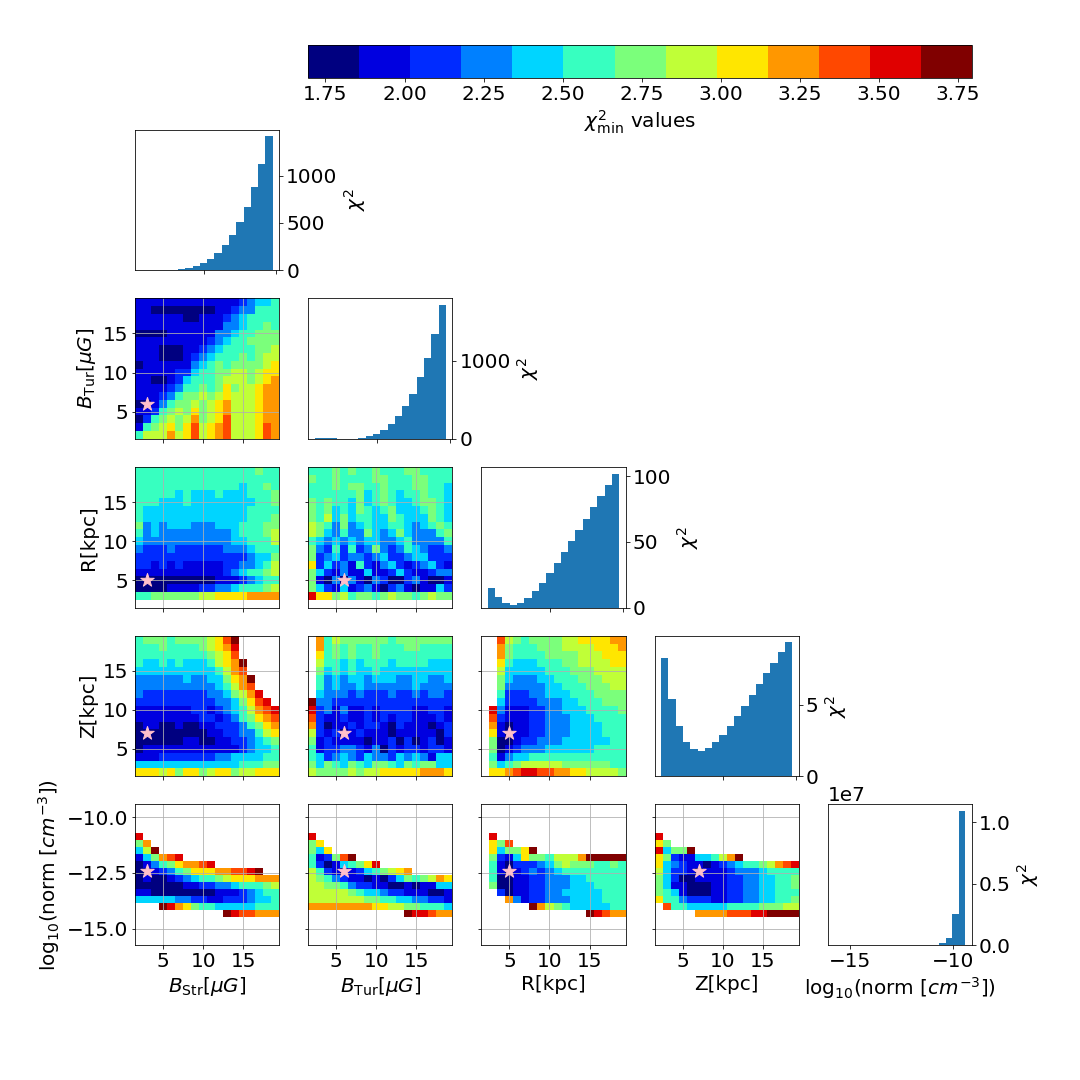
\includegraphics[width = 10cm]{Images/Jan20_Chsq_dof_Para_Scan_1_9_3_elec_den_norm_10GeV.png}
        \caption{\Vasu{I think we do not need this plot for the paper. i can put it in my thesis. Please let me know what you think.}}
        \label{fig:my_label}
\end{figure}


\newpage
\section{Appendix A}\label{Appendix_A}
As discussed in section(\ref{Synchrotron_theory}) the line of sight components for Stokes parameters is given by:
\begin{eqnarray}
Q^l_{\rm in} = ({J_{\perp}^l} - J_{\parallel}^l) \ {\cos}(2\Psi^l_{\rm in}) \ \\ U^l_{\rm in} = ({J_{\perp}^l} - J_{\parallel}^l) \ {\sin}(2\Psi^l_{\rm in}) \ .
\end{eqnarray}
We can take two test cases (I \& II) given in figure(\ref{fig_tot_intensity}) and figure (\ref{fig_pol_intensity}) respectively.We consider that there are two steps along a line of sight for which ${J_{\perp}^{(1,2)}}$ = 0.85 and $J_{\parallel}^{(1,2)}$  = 0.15. 
\\ In case I the angles $\Psi_{\rm in}^{(1,2)}$ = $90^{\circ}$ \& $0^{\circ}$. The resultant value of $I_{\rm pol}$ = 0 by virtue of eq.(\ref{eq_I_pol}) and we only have a contribution in $I_{\rm tot}$. This implies that for case I the resultant emission is seen only in total intensity since the values of $J_{\perp}^{\rm tot}$ = $J_{\parallel}^{\rm tot}$. 
\\ In case II we apply similar calculations to case I however, now the angles are $\Psi_{\rm in}^{(1,2)}$ = $90^{\circ}$ \& $45^{\circ}$. This in turn results in contribution to both polarised emission $I_{\rm pol}$ and total intensity $I_{\rm tot}$. Thus the values of $J_{\perp}^{\rm tot} \neq J_{\parallel}^{\rm tot}$. In figure(\ref{fig_pol_intensity}) we only show polarised intensity for simplicity however, there will be both total intensity and polarised intensity present.
\begin{figure}[h!]
     \centering
     \begin{subfigure}{0.4\textwidth}
         \centering
         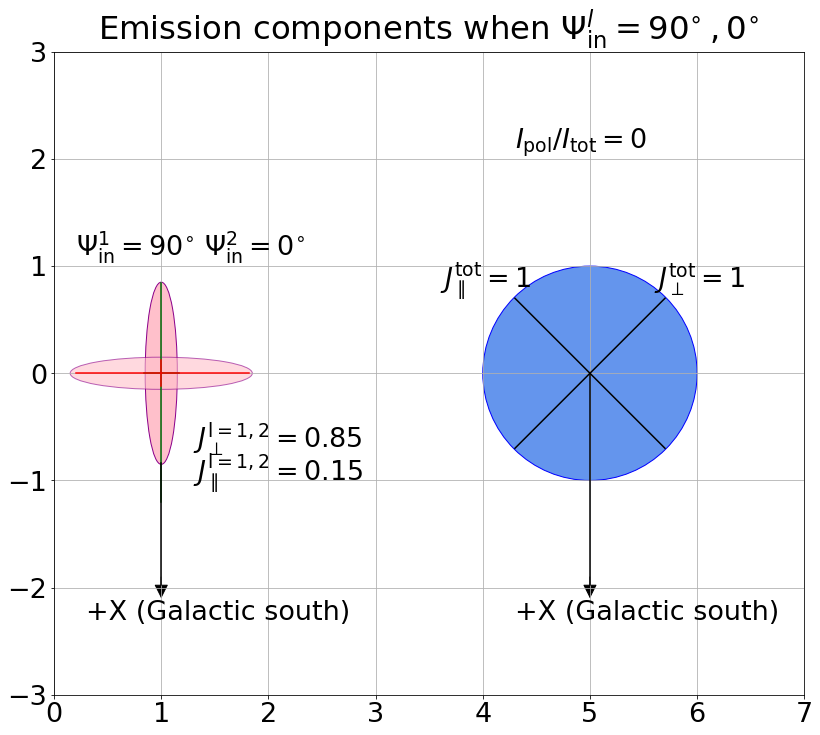
\includegraphics[width = 7cm]{Images/Total_intensity_Ellipses_circles_emissions.png}
         \caption{Case I - Total intensity}
         \label{fig_tot_intensity}
     \end{subfigure}
  \hfill
    \begin{subfigure}{0.4\textwidth}
         \centering
         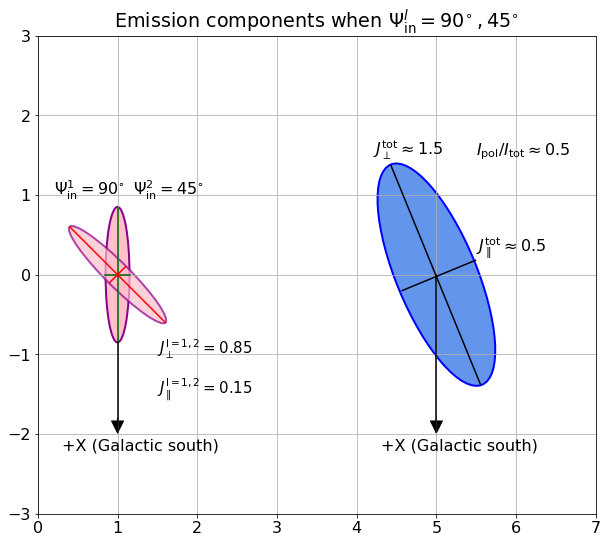
\includegraphics[width = 7cm]{Images/Pol_intensity_Ellipses_circles_emissions.png}
         \caption{Case II - Polarised intensity}
         \label{fig_pol_intensity}
     \end{subfigure}
     \hfill
    \caption{Simplified diagram of emission components for total and polarised intensities in terms of the polarisation ellipses.}
\end{figure}

\newpage
\section{Appendix B}\label{Appendix_B}
As discussed in section ~\ref{GMF} we generate the turbulent fields for our model using CRPropa3 ~\cite{CRPropa3_2016}. We the minimum and maximum wavelength we use to generate these fields are 
$L_{min}$ = 200 pc and $L_{max}$ = 400 pc and $L_{coh} \approx $~150 kpc. One of the major reasons why we do not have enough decades covered for the wavelength is because of the time it takes to generate these fields using CRPropa. 
We looked at power spectrum for different realisations of the turbulent field. In figure ~\ref{fig:PowerSpectrum} we plot power spectrum in X,Y and Z directions by averaging over the other two directions. We chose this particular realisation since it followed closely a power law spectrum of index (5/3). 
\begin{figure}[h!]
    \centering
    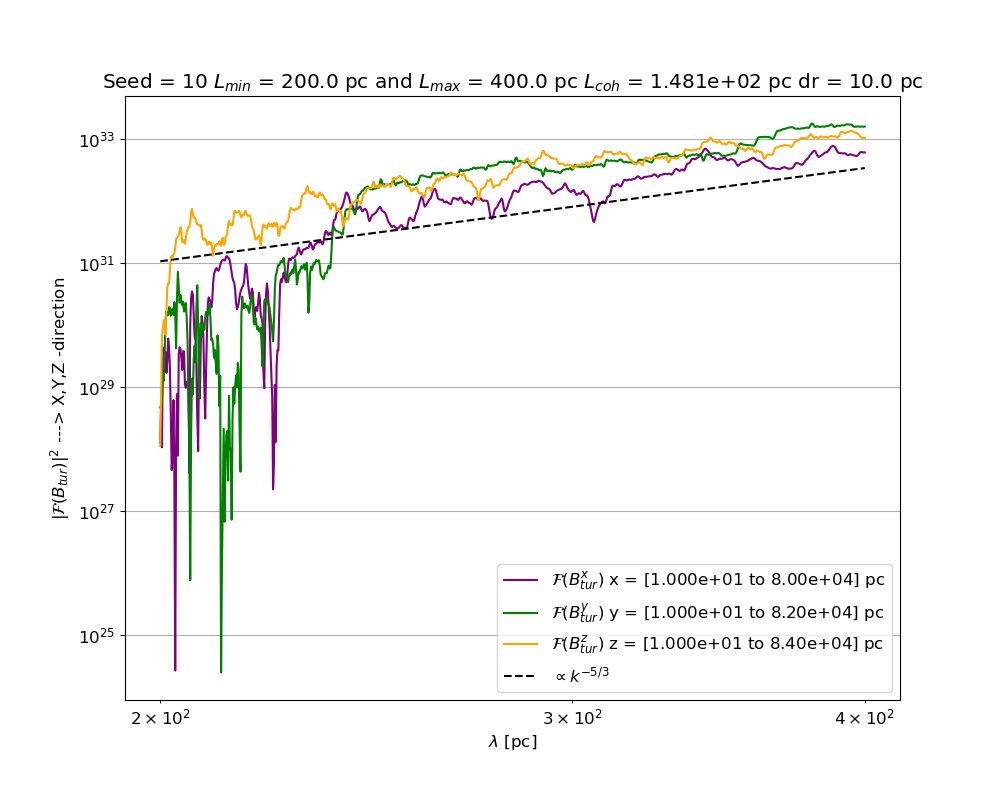
\includegraphics[width = 12cm]{Images/Jan3_Test_PowerSpectrum_vs_lambda_seed_10.png}
    \caption{Power spectrum plot versus wavelength for X, Y and Z direction.}
    \label{fig:PowerSpectrum}
\end{figure}

\iffalse

\newgeometry{top=20mm, bottom=20mm,lmargin=1.mm,rmargin=1.mm} 
\begin{figure}[h!]
    \centering
    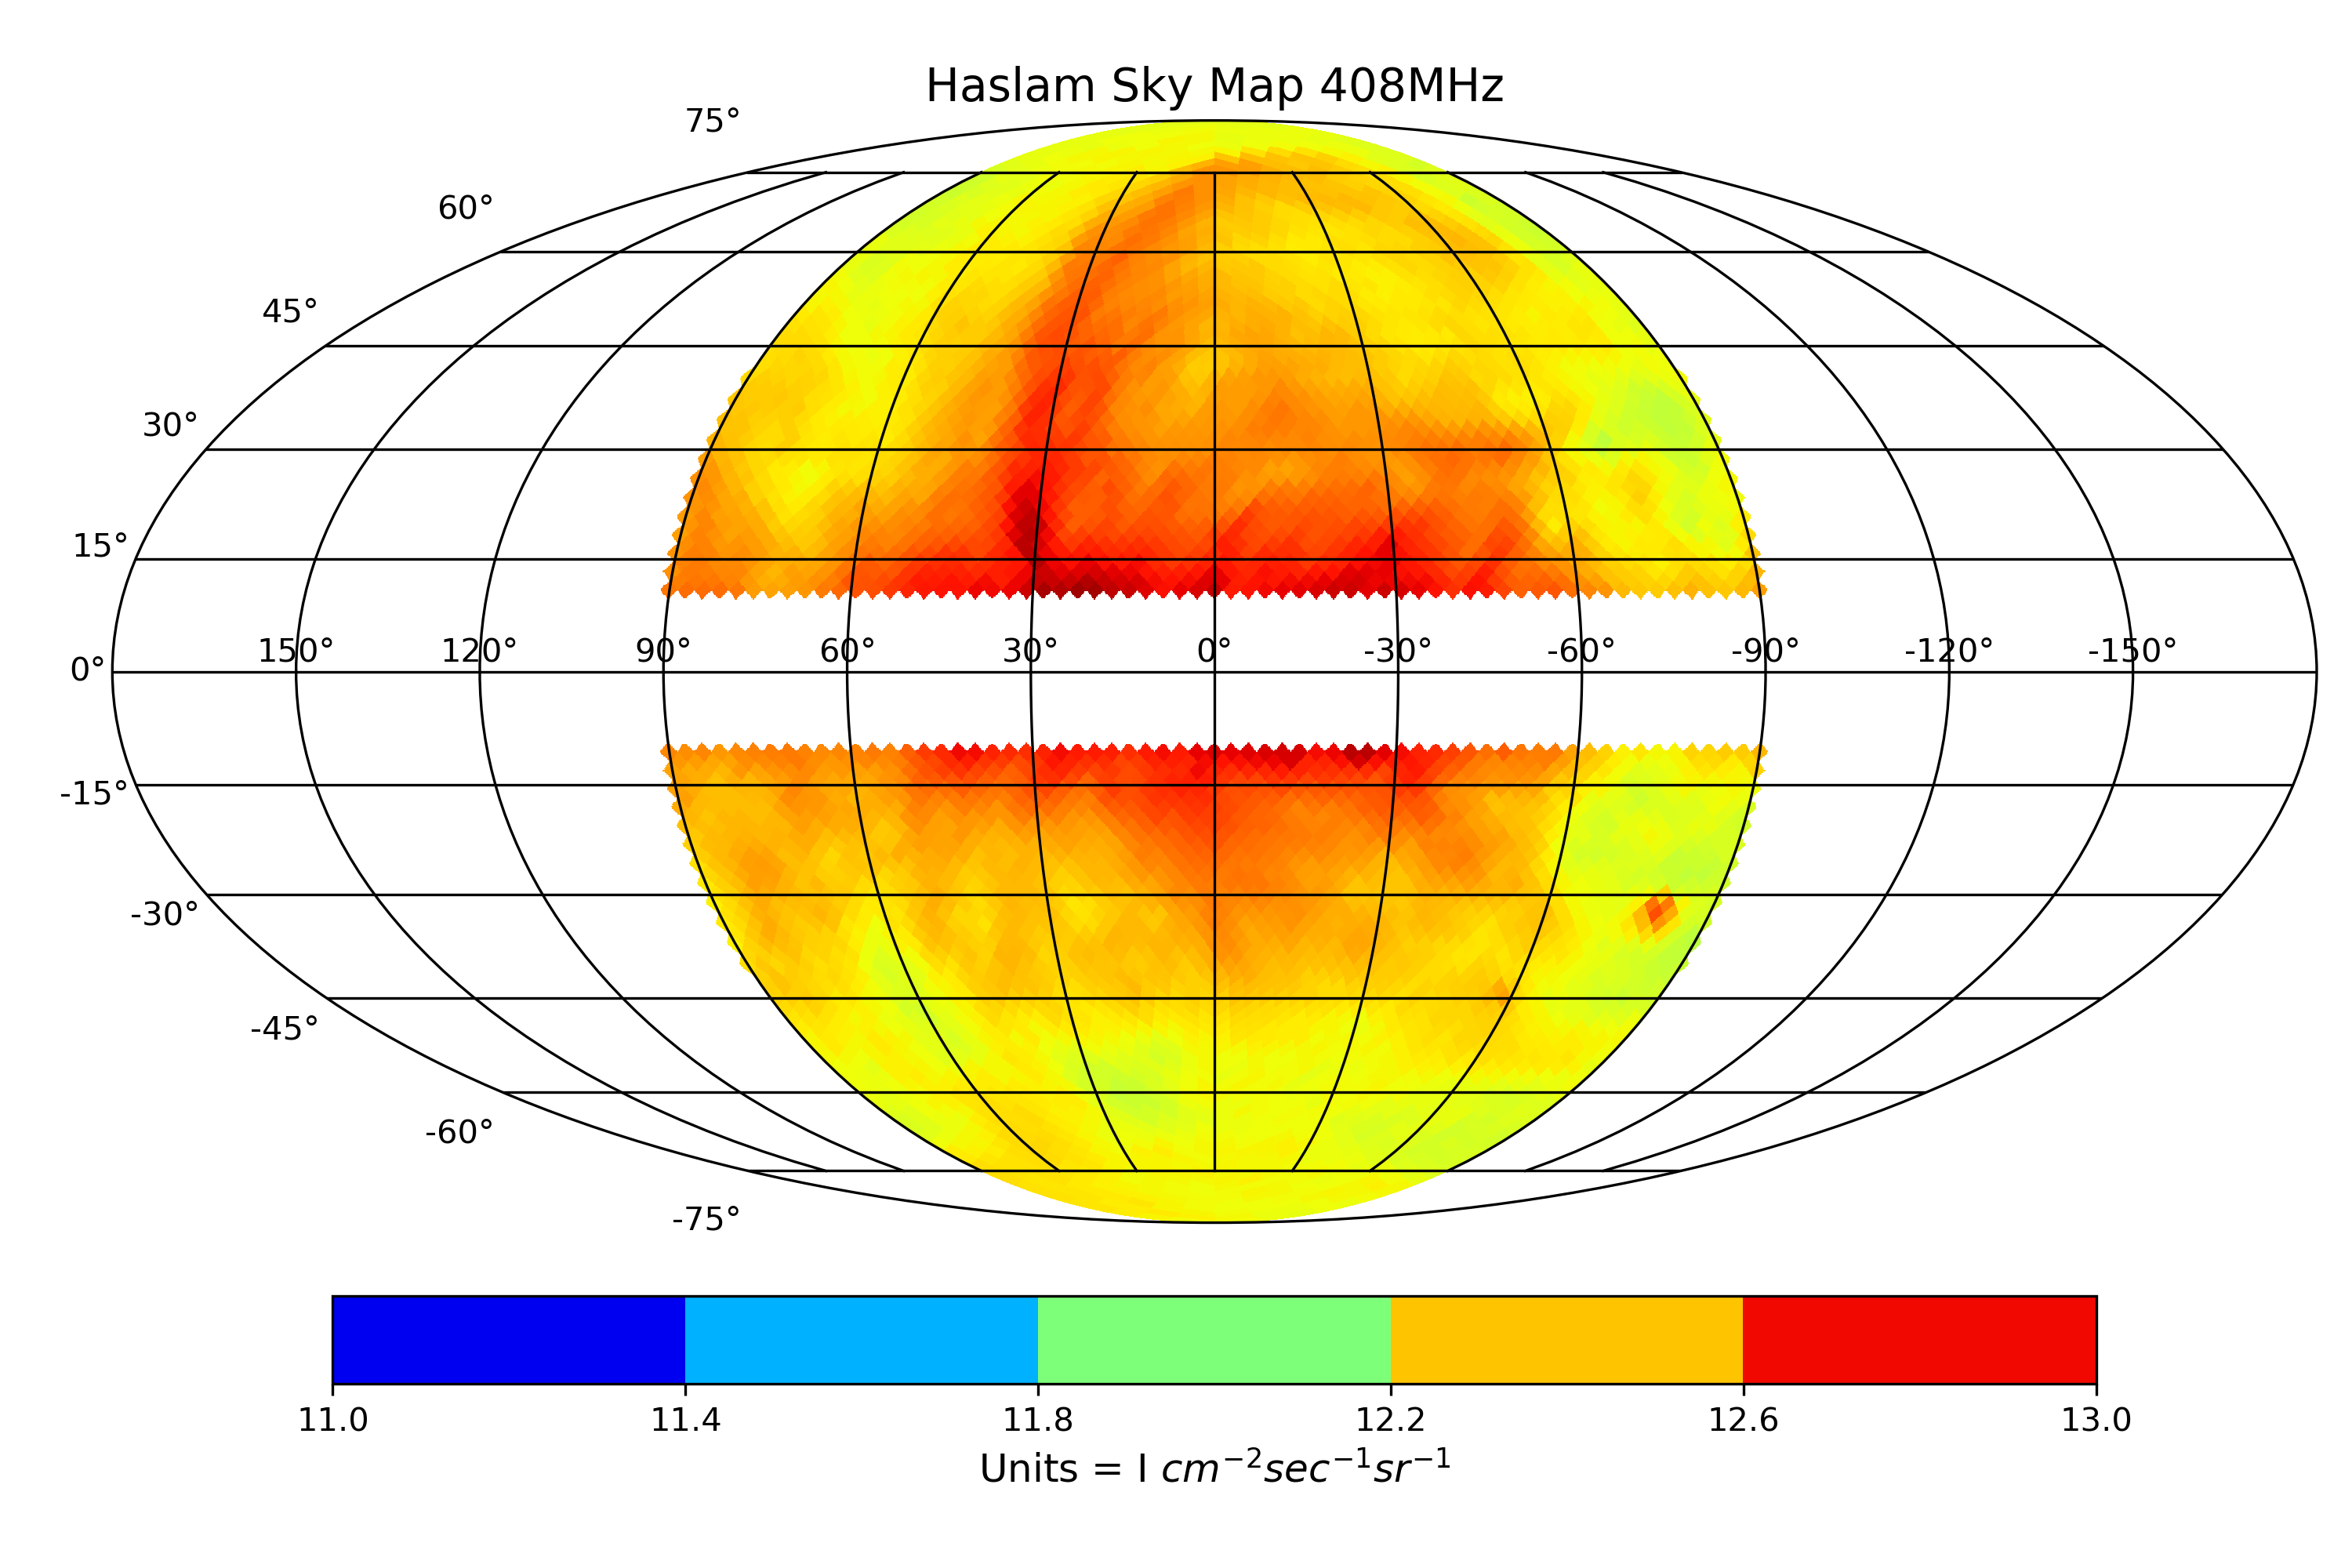
\includegraphics[width = 10cm]{Images/Haslam_408MHz.png}
    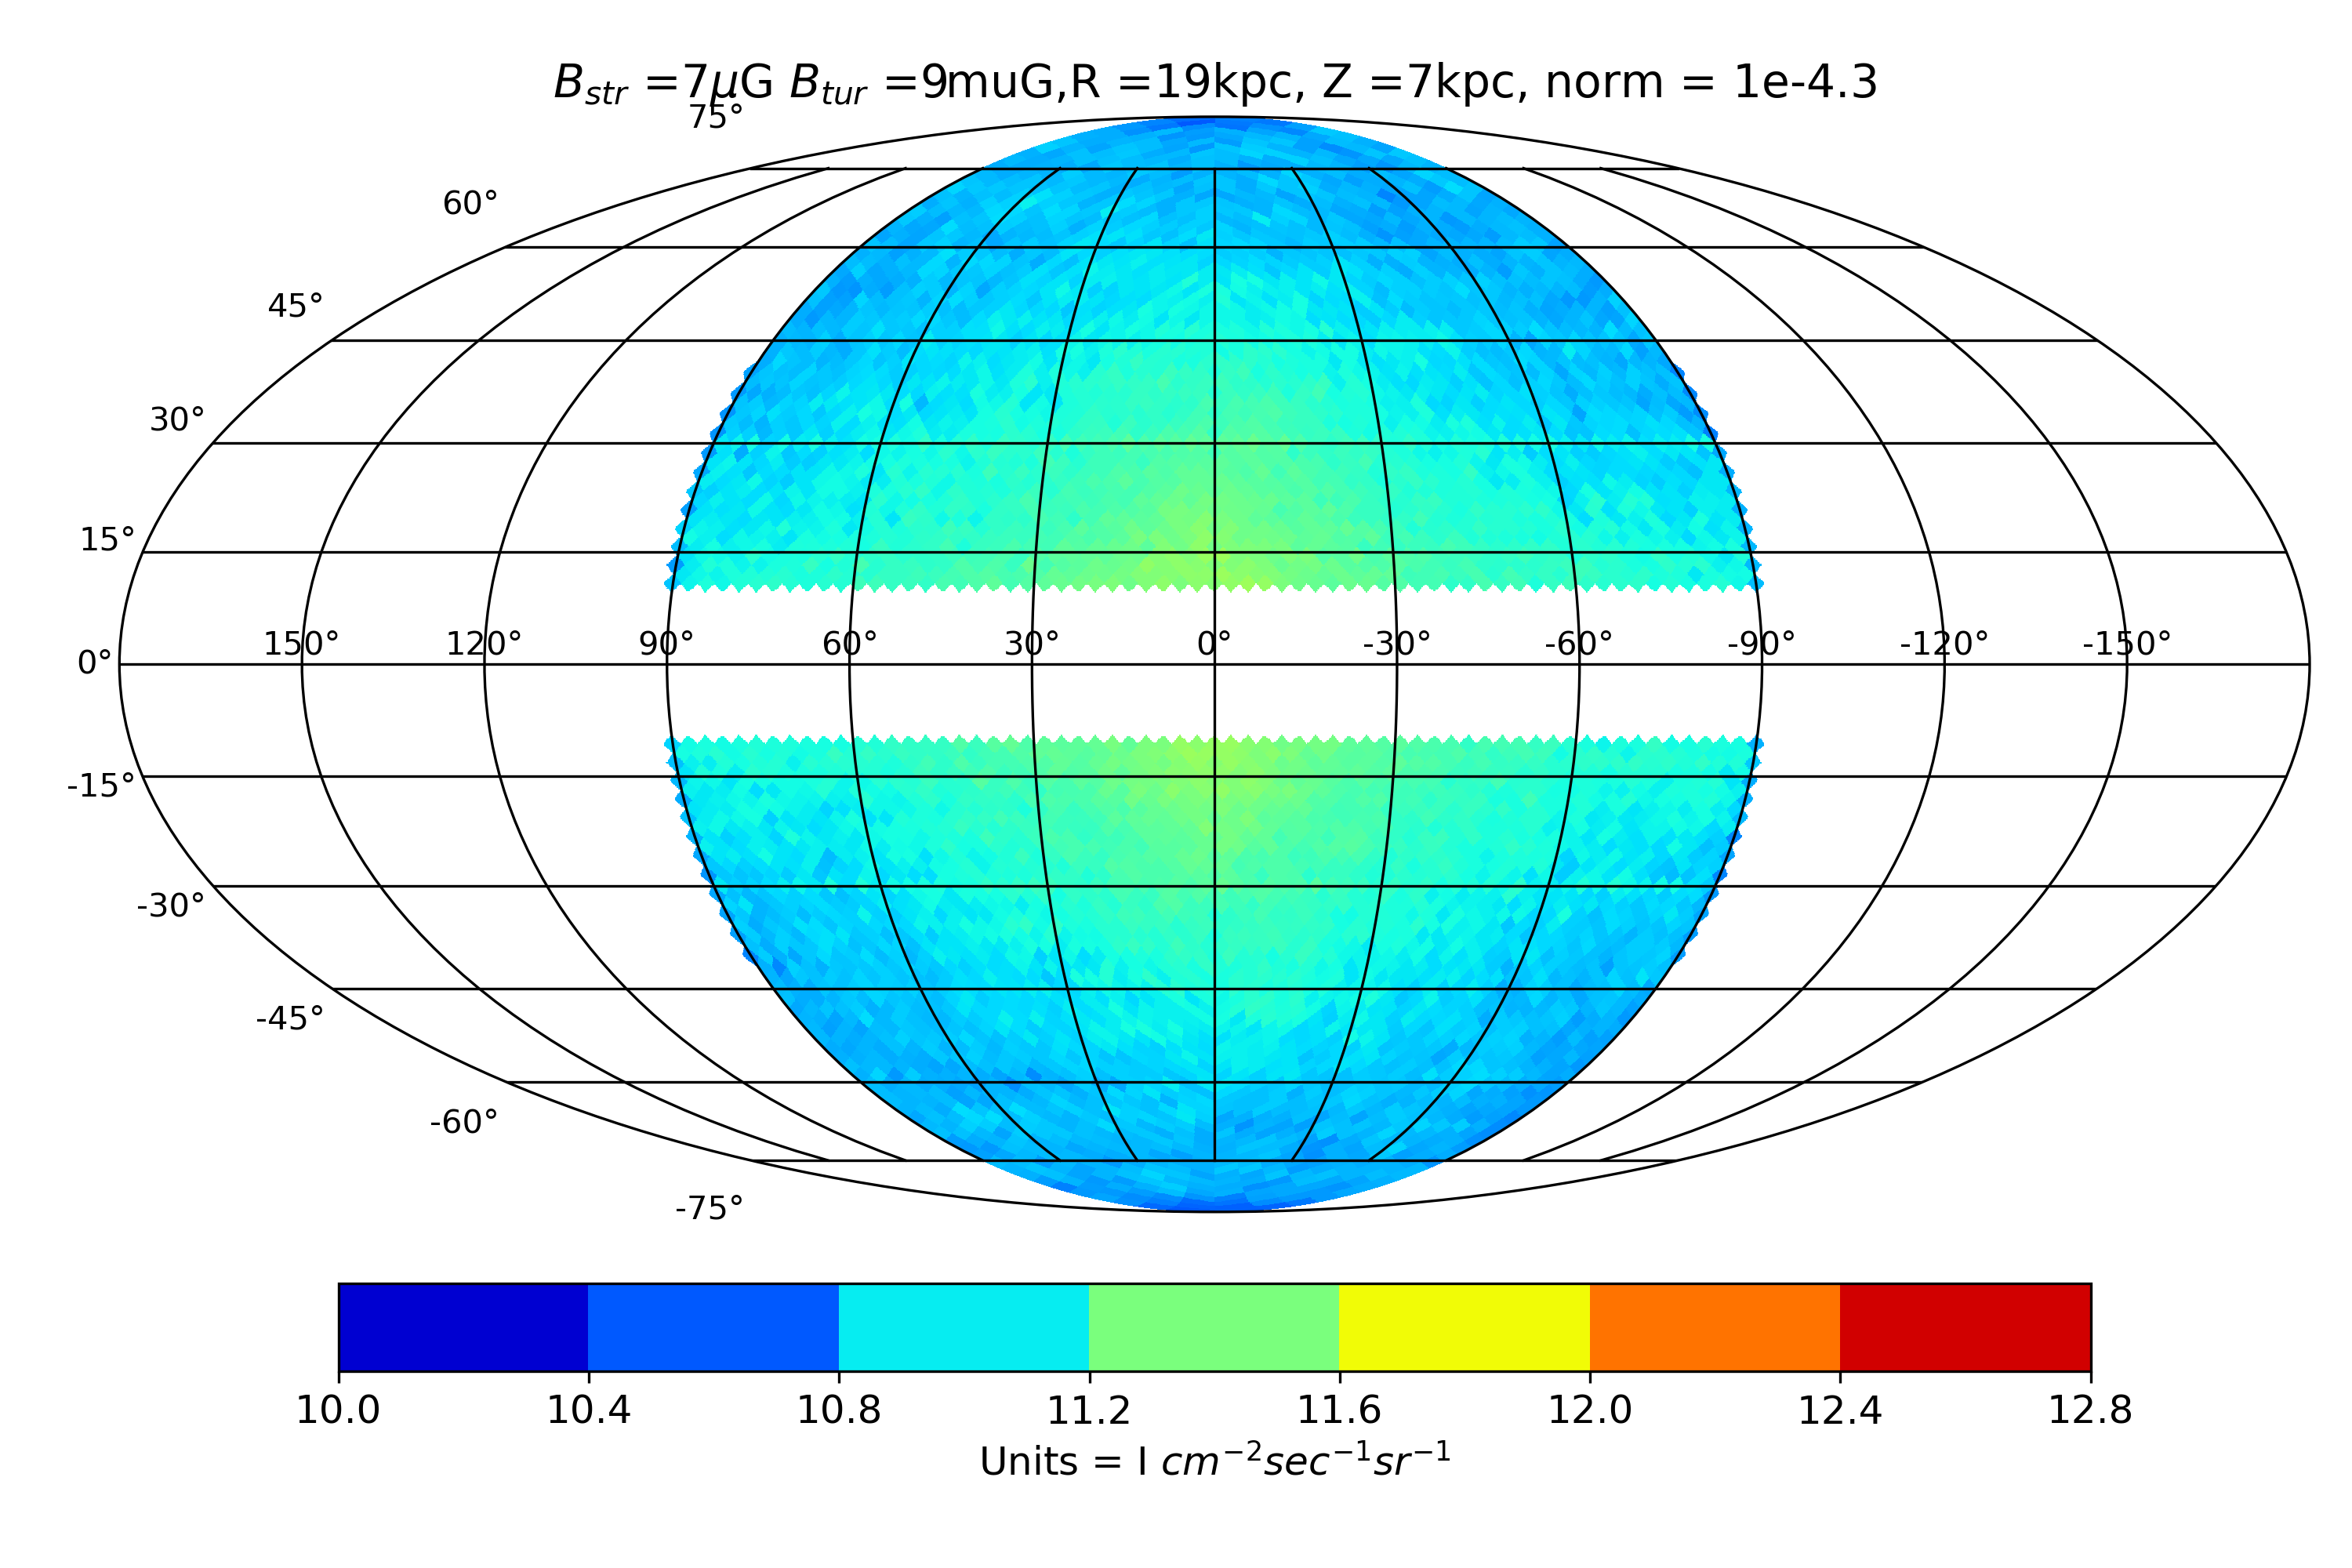
\includegraphics[width =
    10cm]{Images/408MHz_TI_Spec_Ind_3.0_Bstr_7_Btur_9_R_19_Z_7_norm_4.3.png}
 %   \includegraphics[width = 10cm]{Images/408MHz_TI_Spec_Ind_3.3_Bstr_5_Btur_10_R_12_Z_7.png}
    \caption{In figure Haslam data is shown top left, toy model total intensity map top right and in the bottom JF12 skymaps. The disc field is removed from this skymap and it includes Xfield, toroidal halo and turbulent fields.All calculated at $408$MHz. \Andrew{Color bar scales should have a fixed ranged (to allow easy comparison between maps)}}
    \label{fig:my_label}
\end{figure}
\newpage

\fi


\end{document}
